\documentclass{report}
\usepackage{amsmath}
\usepackage{enumerate}
\usepackage{tocloft}
\usepackage{graphicx}
\usepackage{hyperref}
\usepackage{amssymb}
\usepackage{mathrsfs}
\usepackage{physics}
\usepackage{multicol}
\usepackage{esint}

\graphicspath{{MC/images/}{LA/images/}}
% fix for table of contents spacing
\cftsetindents{section}{1em}{3em}
% table of contents links
\hypersetup{
    colorlinks,
    citecolor=black,
    filecolor=black,
    linkcolor=black,
    urlcolor=black
}

% shortcuts for the standard unit vectors
\newcommand{\ihat}{\:\boldsymbol{\hat{\textbf{i}}}}
\newcommand{\jhat}{\:\boldsymbol{\hat{\textbf{j}}}}
\newcommand{\khat}{\:\boldsymbol{\hat{\textbf{k}}}}

% shortcuts for arrows when doing row operations
\newcount\arrowcount
\newcommand\arrows[1]{
        \global\arrowcount#1
        \ifnum\arrowcount>0
                \begin{matrix}
                \expandafter\nextarrow
        \fi
}
\newcommand\nextarrow[1]{
        \global\advance\arrowcount-1
        \ifx\relax#1\relax\else \xrightarrow{#1}\fi
        \ifnum\arrowcount=0
                \end{matrix}
        \else
                \\
                \expandafter\nextarrow
        \fi
}

% shortcut for bold
\def\*#1{\mathbf{#1}}

\begin{document}

\title{\Large{\textbf{MCLA Concice Review}}}
\author{eMeSsBee}
\date{May 2020}

\pagenumbering{roman}
\maketitle
\tableofcontents

\clearpage
\pagenumbering{arabic}

\part{Multivariable Calculus}

\setcounter{chapter}{10}
\chapter{Parametric Equations and Polar Coordinates}

\section{Curves Defined by Parametric Equations}

$x$ and $y$ are given as functions of a third variable $t$,
a \textbf{parameter}, by the equations

$$ x = f(t) \qquad y = g(t) $$

Each value of $t$ determines a point ($x$, $y$).
As $t$ varies, the point ($x$, $y$) = ($f(t)$, $g(t)$)
varies and traces out a curve $C$, a \textbf{parametric curve}.

\subsection*{Example}

Sketch the curve defined by
$$ x = t^2-2t \qquad y = t+1 $$

\subsection*{Solution}
Use values for $t$ and plug those into $x(t)$ and $y(t)$ to get points ($x$, $y$)

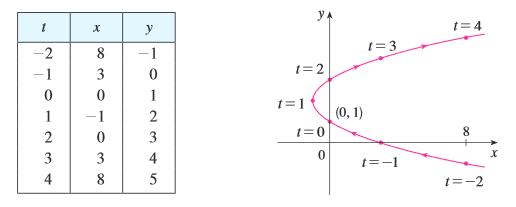
\includegraphics{example11-1-1}

\section{Calculus with Parametric Curves}

\subsection*{Tangents}
$f$ and $g$ are differentiable functions and we want to find the
tangent line at a point ($f(t)$, $g(t)$). The Chain Rule gives

$$ \frac{dy}{dt} = \frac{dy}{dx} \cdot \frac{dx}{dt} $$

$$ \frac{dy}{dx} = \frac{\frac{dy}{dt}}{\frac{dx}{dt}} \qquad if \: \frac{dx}{dt} \neq 0$$

$d^2y/dx^2$ can be found by replacing $y$ with $dy/dx$ in the equation above

$$ \frac{d^2y}{dx^2} = \frac{d}{dx}\left(\frac{dy}{dx}\right) = \frac{\frac{d}{dt}(\frac{dy}{dx})}{\frac{dx}{dt}} $$

\subsection*{Example}
Find the tangent to the cycloid $x=r(\theta - sin\: \theta)$, $y=r(1-cos\: \theta)$
at the point where $\theta=\pi/3$.

\subsection*{Solution}
The slope of the tangent is
$$\frac{dy}{dx}=\frac{dy/d\theta}{dx/d\theta}=\frac{r\: sin\: \theta}{r(1-cos\: \theta)}
    =\frac{sin\: \theta}{1-cos\: \theta}$$
When $\theta=\pi /3$, we have
$$x=r\left(\frac{\pi}{3}-sin\frac{\pi}{3}\right)=r\left(\frac{\pi}{3}-\frac{\sqrt{3}}{2}\right)
    \qquad y=r\left(1-cos\frac{\pi}{3}\right)=\frac{r}{2}$$
and
$$\frac{dy}{dx}=\frac{sin(\pi/3)}{1-cos(\pi/3)}=\sqrt{3}$$
Therefore the slope of the tangent is $\sqrt{3}$ and its equation is
$$y-\frac{r}{2}=\sqrt{3}\left(x-\frac{r\pi}{3}+\frac{r\sqrt{3}}{2}\right)$$

\subsection*{Areas}
Area under a curve $y = F(x)$ form $a$ to $b$ is $A = \int_a^b F(x) dx$.
If the curve is traced out with the parametric equations $f(t)$ and $g(t)$,
we can calculate the area by using the Substitution Rule for Definite Integrals:

$$A=\int_a^b ydx = \int_\alpha^\beta g(t)f'(t)dt$$

\subsection*{Example}
Find the area under one arch of the cycloid
$$x=r(\theta-sin\: \theta) \qquad y=r(1-cos\: \theta)$$

\subsection*{Solution}
One arch of the cycloid is given by $0\leq \theta \leq 2\pi$. Using the substitution
rule with $y=r(1-cos\: \theta)$ and $dx=r(1-cos\: \theta)d\theta$, we have
$$A=\int_0^{2\pi r}y\: dx=\int_0^{2\pi r}r(1-cos\: \theta)r(1-cos\: \theta)d\theta$$
$$=r^2(\frac{3}{2}\cdot 2\pi)=3\pi r^2$$

\subsection*{Arc Length}
To find the length $L$ of a curve $C$ in the from $y=F(x)$
$$ L = \int_a^b \sqrt{1+(\frac{dy}{dx})^2} dx $$

Suppose C can also be described with parametric equations, we obtain
$$ L = \int_a^b \sqrt{1+\left(\frac{dy}{dx}\right)^2} dx = \int_\alpha^\beta \sqrt{1+(\frac{dy/dt}{dx/dt})^2}\frac{dx}{dt}dt $$

\subsection*{Theorem}
If a curve C is described by the parametric equations $x=f(t)$, $y=g(t)$,
$\alpha \leq t \leq \beta$, where $f'$ and $g'$ are continuous on [$\alpha$,$\beta$]
and $C$ is traversed exactly once as $t$ increases from $\alpha$ to $\beta$, then
the length of $C$ is
$$ L = \int_a^b \sqrt{\left(\frac{dx}{dt}\right)^2+\left(\frac{dy}{dt}\right)^2} dt $$

\subsection*{Example}
Find the length of one arch of the cycloid $x=r(\theta-sin\theta)$, $y=r(1-cos\:\theta)$

\subsection*{Solution}
Since
$$\frac{dx}{d\theta}=r(1-cos\:\theta) \qquad \frac{dy}{d\theta}=rsin\:\theta$$
we have
$$L=\int_0^{2\pi}\sqrt{\left(\frac{dx}{d\theta}\right)^2+\left(\frac{dy}{d\theta}\right)^2}d\theta$$
$$=\int_0^{2\pi}\sqrt{r^2(1-cos\:\theta)^2+r^2sin^2\theta}d\theta$$
$$=r\int_0^{2\pi}\sqrt{2(1-cos\:\theta)}d\theta$$
$$=2r[2+2]=8r$$

\subsection*{Surface Area}
Suppose a curve $C$ is rotated about the $x$-axis. If $C$ si traversed exactly
once as $t$ increases from $\alpha$ to $\beta$, then the area of the surface is given by
$$ S = \int_\alpha^\beta 2 \pi y \sqrt{\left(\frac{dx}{dt}\right)^2+\left(\frac{dy}{dt}\right)^2} dt $$

The general symbolic formulas $S=\int 2 \pi y ds$ and $S = \int 2 \pi x ds$
are still valid, but for parametric curves we use
$$ ds = \sqrt{\left(\frac{dx}{dt}\right)^2+\left(\frac{dy}{dt}\right)^2} dt $$

\subsection*{Example}
Show that the surface area of a sphere of radius $r$ is $4\pi r^2$.

\subsection*{Solution}
The sphere is obtained by rotating the semicircle
$$x=rcos\:t \qquad y=rsin\:t \qquad 0\leq t\leq \pi$$
about the $x$-axis. Then, we get
$$S=\int_0^\pi 2\pi r\: sin\:t\sqrt{(-rsin\:t)^2+(rcos\:t)^2}dt$$
$$=2\pi r^2\int_0^\pi sin\:t\:dt = 2\pi r^2(-cos\:t)]_0^\pi = 4\pi r^2$$

\section{Polar Coordinates}
The Polar Coordinate System starts witha point in the plan called the \textbf{pole}
and is labeled $O$. Then we draw a ray starting at $O$ called the \textbf{polar axis}.
This corresponds to the positive $x$-axis in Cartesian coordinates. \par

$r$ is the ditsance from $O$ to $P$ and $\theta$ is the angle between the polar axis
and the line $OP$. The \textbf{polar coordinates} of $P$ are in the form ($r$, $\theta$), \par

If a point $P$ has Cartesian coordinates ($x$, $y$) and polar coordinates ($r$, $\theta$)
$$ cos \: \theta = \frac{x}{r} \qquad y = r sin \: \theta $$

and so
$$ x=r cos \: \theta \qquad y = r sin \: \theta$$

To find $r$ and $\theta$ when $x$ and $y$ are known, we use
$$ r^2 = x^2 + y^2 \qquad tan \: \theta = \frac{y}{x} $$

\subsection*{Example}
What curve is represented by the polar equation $r$=2?

\subsection*{Solution}
The equation $r$ = $a$ represents a circle with center $O$ and radius $|a|$.
The polar equation represents a circle about the origin with a radius of 2.

\subsection*{Example}
What curve is represented by the polar equation $\theta$=1?

\subsection*{Solution}
This curve consists of all points ($r$, $\theta$) such that $\theta$ is 1 radian.
It is a straight line that passes through $O$ and makes an angle of 1 radian with
the polar axis.

\subsection*{Tangents to Polar Curves}
To find a tangent line to a polar curve $r$ = $f(\theta)$, we write its parametric equations as
$$ x=r cos \: \theta=f(\theta)\:cos \: \theta \qquad y = r sin \: \theta = f(\theta)\:sin \: \theta$$

Then, using the method of finding slopes of parametric curves and the Product Rule, we have
$$ \frac{dy}{dx}=\frac{\frac{dy}{d\theta}}{\frac{dx}{d\theta}}=\frac{\frac{dr}{d\theta}sin\:
        \theta+r\:cos\:\theta}{\frac{dr}{d\theta}cos\:\theta-r\:sin\:\theta} $$

\section{Areas and Lengths in Polar Coordinates}

Using the formula for the area of a sector of a circle
$$ A=\frac{1}{2}r^2\theta $$

the formula for the area $A$ of the polar region $R$ is
$$ A=\int_a^b\frac{1}{2}[f(\theta)]^2 \: d\theta  = \int_a^b\frac{1}{2}r^2 \: d\theta$$

\subsection*{Arc Length}

To find the length of a polar curve $r$=$f(\theta)$, we write the parametric equations as
$$ x=r cos \: \theta=f(\theta)\:cos \: \theta \qquad y = r sin \: \theta = f(\theta)\:sin \: \theta$$

Using the Product Rule and differentiating with respect to $\theta$, we obtain
$$ \frac{dx}{d\theta}=\frac{dr}{d\theta}\:cos\:\theta-r\:sin\:\theta \qquad \frac{dy}{d\theta}=
    \frac{dr}{d\theta}\:sin\:\theta+r\:cos\:\theta $$

so, using $cos^2\theta + sin^2\theta = 1$, we have
$$ \left(\frac{dx}{d\theta}\right)^2 + \left(\frac{dy}{d\theta}\right)^2 = \frac{dr}{d\theta})^2 + r^2$$

Therefore the length of a curve is
$$ L=\int_a^b\sqrt{r^2+\left(\frac{dr}{d\theta}\right)^2}\:d\theta $$

\section{Conic Sections}

\subsection*{Parabolas}
An equation of the parabola with focus (0, $p$) and directrix $y=-p$ is
$$ x^2=4py $$

\subsection*{Ellipses}
The ellipse
$$ \frac{x^2}{a^2}+\frac{y^2}{b^2}=1 \qquad a \leq b > 0 $$
has focus ($\pm c$, 0), where $c^2=a^2-b^2$, and vertices ($\pm a$, 0) \\
The ellipse
$$ \frac{x^2}{b^2}+\frac{y^2}{a^2}=1 \qquad a \leq b > 0 $$
has focus (0, $\pm c$), where $c^2=a^2-b^2$, and vertices (0, $\pm a$)

\subsection*{Hyerpbolas}
The hyperbola
$$ \frac{x^2}{a^2}-\frac{y^2}{b^2}=1 $$
has foci($\pm c$, 0), where $c^2=a^2+b^2$, vertices ($\pm a$, 0), and
asymptomes $y=\pm(b/a)x$. \\
The hyperbola
$$ \frac{y^2}{a^2}-\frac{x^2}{b^2}=1 $$
has foci(0, $\pm c$), where $c^2=a^2+b^2$, vertices (0, $\pm a$), and
asymptomes $y=\pm(a/b)x$.

\section{Conic Sections in Polar Coordinates}

\subsection*{Theorem}
Let $P$ be a fixed point (the \textbf{focus}) and $l$ be a fixed line (called the \textbf{directrix})
in a plane. Let $e$ be a fixed positive number (called the \textbf{eccentricity}).
The set of all points $P$ in the plane such that
$$ \frac{|PF|}{|Pl|}=e $$
The conic is \par
(a) an ellipse if $e <$ 1 \par
(b) a parabola if $e =$ 1  \par
(c) a hyperbola if $e >$ 1

\subsection*{Theorem}
A polar equation of the form
$$ r=\frac{ed}{1\pm e\:cos\:\theta} \quad or \quad r=\frac{ed}{1\pm e\:sin\:\theta} $$
represents a conic section the eccentricity $e$. The conic is an ellipse
if $e <$ 1, a parabola if $e =$ 1, or a hyperbola if $e >$ 1.

\subsection*{Polar}
The polar equation of an ellipse with focus at the origin, emimajor axis $a$,
eccentricity $e$, and directrix $x=d$ can be written in the form
$$ r=\frac{a(1-e^2)}{1+e\:cos\:\theta} $$

The \textbf{perihelion distance} from a planet to the sun is $a(1-e)$
and the \textbf{aphelion distance} is $a(1+e)$.
\chapter{Infinite Sequences and Series}

\section{Sequences}
A \textbf{sequence} can be thought of as a list of numbers in definite order:
$$ a_1, a_2, a_3, a_4, \dots, a_n,\dots $$
which can also be denoted by
$$ \{a_n\} \qquad or \qquad \{a_n\}_{n=1}^\infty $$

\subsection*{Definition}
A sequence $\{a_n\}$ has the \textbf{limit} $L$ and we write
$$ \lim_{n \to \infty}a_n = L \qquad or \qquad a_n \rightarrow L \quad as \quad n \rightarrow \inf $$
if $\lim_{n \to \infty}a_n$ exists, we say the sequence \textbf{converges}).
Otherwise, we say the sequence \textbf{diverges}.

\subsection*{Definition}
A sequence $\{a_n\}$ has the \textbf{limit} $L$ and we write
$$ \lim_{n \to \infty}a_n = L \qquad or \qquad a_n \rightarrow L \quad as \quad n \rightarrow \inf $$
if for every $\epsilon >$ 0 there is corresponding integer $N$ such that
$$ if \quad n>N \quad then \quad |a_n - L|<\epsilon $$

\subsection*{Theorem}
if $\lim_{x \to \infty}f(x)=L$ and $f(n)=a_n$ when $n$ is an integer,
then $\lim_{n \to \infty}a_n=L$

\subsection*{Definition}
$\lim_{n \to \infty}a_n=\infty$ means that for every positive number $M$
there is an integer $N$ such that
$$ if \quad n>N \quad then \quad a_n>M $$

\subsection*{Theorem}
If $\lim_{n \to \infty}|a_n|=0$, then $\lim_{a \to \infty}a_n=0$

\subsection*{Theorem}
If $\lim_{n \to \infty}a_n=L$ and the function $f$ is continuous at $L$, then
$$ \lim_{n \to \infty}f(a_n) = f(L) $$

A sequence \{$r^n$\} is convergent if $-1<r\leq1$ and divergent for all other values of $r$.
$$ \lim_{n \to \infty}r^n =
    \begin{cases}
        0 & \text{if $-1<r\leq1$} \\
        1 & \text{if $r=1$}
    \end{cases} $$

\subsection*{Example}
Find $\lim_{n\to \infty}sin(\pi /n)$.

\subsection*{Solution}
Because the sine function is continuous at 0,
$$\lim_{n\to \infty}sin(\pi /n)=sin\left(\lim_{n\to \infty}(\pi /n)\right)=sin\:0=0$$

\subsection*{Definition}
A sequence \{$a_n$\} is called \textbf{increasing} if $a_n < a_{n+1}$
for all $n \geq 1$, that is $a_1<a_2<a_3<\dots$. It is called \textbf{decreasing}
if $a_n>a_{n+1}$ for all $n \geq 1$. A sequence is \textbf{monotonic}
if it's either increasing or decreasing.

\subsection*{Example}
Show that the sequence $a_n-\cfrac{n}{n^2+1}$ is decreasing.

\subsection*{Solution}
Consider the function $f(x)=\cfrac{x}{x^2+1}$:
$$f'(x)=\frac{x^2+1-2x^2}{(x^2+1)^2}=\frac{1-x^2}{(x^2+1)^2}<0$$
Thus $f$ is decreasing on $(1,\infty)$ and so $f(n)>f(n+1)$. Therefore ${a_n}$ is decreasing.

\subsection*{Definition}
A sequence \{$a_n$\} is \textbf{bounded above} if there is a number $M$ such that
$$ a_n \leq M \qquad for all n \geq 1 $$
It is \textbf{bounded below} if there is a number $m$ such that
$$ m \leq a_n \qquad for all n \geq 1 $$
It is bounded above and below, then \{$a_n$\} is a \textbf{bounded sequence}

\subsection*{Monotonic Sequence Theorem}
Every bounded, monotonic sequence is convergent.

\section{Series}
If we try to add the terms if an infinite sequence $\{a_n\}_{n=1}^\infty$
we get an expression of the form
$$ a_1+a_2+a_3+\dots+a_n+\dots $$
which is an \textbf{infinite series} (or just a \textbf{series}) and is denoted by
$$ \sum_{n=1}^{\infty} a_n \qquad or \qquad \sum a_n $$

\subsection*{Definition}
Given a series $\sum_{n=1}^n a_n = a_1+a_2+a_3+\dots$, let $s_n$ denote
its $n$th partial sum:
$$ s_n=\sum_{i=1}^n a_i = a_1+a_2+\dots + a_n $$
If the sequence \{$s_n$\} is convergent and $\lim_{n \to \infty} s_n =s$
exists as a real number, then the series $\sum a_n$ is called
\textbf{convergent} and we write
$$ a_1 + a_2 + \dots + a_n + \dots = s \qquad or \qquad \sum_{n=1}^\infty a_n = s$$
The number $s$ is called the \textbf{sum} of the series. If the sequence
\{$s_n$\} is divergent, then the series is called \textbf{divergent}. \par\null\par
\noindent The geometric series
$$ \sum_{n=1}^\infty ar^{n-1} = a + ar + ar^2 + \dots $$
is convergent if $|r| < 1$ and its sum is
$$ \sum_{n=1}^\infty ar^{n-1}=\frac{a}{1-r} \qquad |r|<1 $$
If $|r| \geq 1$, the geometric series is divergent.

\subsection*{Example}
Is the series $\sum_{n=1}^\infty 2^{2n}3^{1-n}$ convergent or divergent?

\subsection*{Solution}
Let's rewrite the $n$th term of the series in the form $ar^{n-1}$:
$$\sum_{n=1}^\infty 2^{2n}3^{1-n}=\sum_{n=1}^\infty (2^2)^n3^{-(n-1)}=
    \sum_{n=1}^\infty\frac{4^n}{3^{n-1}}=\sum_{n=1}^\infty 4\left(\frac{4}{3}\right)^{n-1}$$
This is a geometric series with $a=4$ and $r=\frac{4}{3}$. Since $r>1$, the series
diverges by (4).

\subsection*{Theorem}
If the series $\sum_{n=1}^\infty a_n$ is convergent, then
$\lim_{n \to \infty} a_n = 0$.

\subsection*{Test for Divergence}
If $\lim_{n \to \infty} a_n$ does not exist or if $\lim_{n \to \infty} a_n \neq 0$,
then the series $\sum_{n=1}^\infty a_n$ is divergent.

\subsection*{Example}
Show that the series $\sum_{n=1}^\infty \frac{n^2}{5n^2+4}$ diverges.

\subsection*{Solution}
$$\lim_{n\to \infty}a_n=lim_{n\to \infty}\frac{n^2}{5n^2+4}=
    lim_{n\to \infty}\frac{1}{5+4/n^2}=\frac{1}{5}\neq0$$
So the series diverges by the Test for Divergence.

\subsection*{Theorem}
If $\sum a_n$ and $\sum b_n$ are convergent series, then so are the series
$\sum ca_n$ (where $c$ is constant), $\sum (a_n+b_n)$, and $\sum(a_n-b_n)$, and
\begin{enumerate}[(i)]
    \item $\sum_{n=1}^\infty ca_n = c\sum_{n=1}^\infty a_n$
    \item $\sum_{n=1}^\infty(a_n+b_n)=\sum_{n=1}^\infty a_n + \sum_{n=1}^\infty b_n$
    \item $\sum_{n=1}^\infty(a_n-b_n)=\sum_{n=1}^\infty a_n - \sum_{n=1}^\infty b_n$
\end{enumerate}

\section{The Integral Test and Estimates of Sums}

\subsection*{The Integral Test}
Suppose $f$ is a continuous, positive, decreasing, function on $[1, \infty)$ and let
$a_n = f(n)$. Then the series $\sum_{n=1}^\infty a_n$ is convergent if and only if
the improper integeral $\int_1^\infty f(x) dx$ is convergent. In other words:
\begin{enumerate}[(i)]
    \item If $\int_1^\infty f(x) dx$ is convergent, then $\sum_{n=1}^\infty a_n$ is convergent.
    \item If $\int_1^\infty f(x) dx$ is divergent, then $\sum_{n=1}^\infty a_n$ is divergent.
\end{enumerate}
The $p$-series $\sum_{n=1}^\infty \frac{1}{n^p}$ is convergent if $p>1$ and divergent if $p \leq 1$.

\subsection*{Example}
Test the series $\sum_{n=1}^\infty\frac{1}{n^2+1}$ for convergence or divergence.

\subsection*{Solution}
The function $f(x)=1/(x^2+1)$ is continuous, positive, and decreasing on $[1,\infty)$
so we use the Integral Test:
$$\int_1^\infty \frac{1}{x^2+1}dx=\lim_{t\to\infty}\int_1^t\frac{1}{x^2+1}dx=
    \lim_{t\to\infty}tan^{-1}x]_1^t$$
$$=\lim_{t\to\infty}\left(tan^{-1}t-\frac{\pi}{4}\right)=\frac{\pi}{2}-\frac{\pi}{4}=\frac{\pi}{4}$$
The integral converges and so the series is convergent/

\section{The Comparison Tests}

\subsection*{The Comparison Test}
Suppose that $\sum a_n$ and $\sum b_n$ are series with positive terms.
\begin{enumerate}[(i)]
    \item If $\sum b_n$ is convergent and $a_n \leq b_n$ for all $n$, then $\sum a_n$ is also convergent.
    \item If $\sum b_n$ is divergent and $a_n \geq b_n$ for all $n$, then $\sum a_n$ is also divergent.
\end{enumerate}

\subsection*{Example}
Determine whether the series $\sum_{n=1}^\infty\frac{5}{2n^2+4n+3}$ converges or diverges.

\subsection*{Solution}
$$\frac{5}{2n^2+4n+3} < \frac{5}{2n^2}$$
We know that
$$\sum_{n=1}^\infty\frac{5}{2n^2}=\frac{5}{2}\sum_{n=1}^\infty\frac{1}{n^2}$$
is convergent because it's a $p$-series with $p=2>1$. Therefore
$$\sum_{n=1}^\infty\frac{5}{2n^2+4n+3}$$
is convergent by part (i) of the Comparison Test

\subsection*{The Limit Comparison Test}
Suppose that $\sum a_n$ and $\sum b_n$ are series with positive terms. If
$$ \lim_{n \to \infty} \frac{a_n}{b_n} = c $$
where $c$ is a finite number and $c>0$, then either both series converge or diverge.

\subsection*{Example}
Test the series $\sum_{n=1}^\infty\frac{1}{2^n-1}$ for convergence or divergence.

\subsection*{Solution}
We use the Limit Comparison Test with
$$a_n=\frac{1}{2^n-1} \qquad b_n=\frac{1}{2^n}$$
and obtain
$$\lim_{n\to\infty}\frac{a_n}{b_n}=\lim_{n\to\infty}\frac{1/(2^n-1)}{1/2^n}=
    \lim_{n\to\infty}\frac{2^n}{2^n-1}=\lim_{n\to\infty}\frac{1}{1-1/2^n}=1>0$$
Since this limit exists and $\sum 1/2^n$ is a convergent geometric series, the given
converges by the Limit Comparison Test.

\section{Alternating Series}
An \textbf{alternating series} is a series whose terms are alternately positive and negative.
$$ 1-\frac{1}{2}+\frac{1}{3}-\frac{1}{4}+\frac{1}{5}-\frac{1}{6}+\dots = \sum_{n=1}^\infty (-1)^{n-1} \frac{1}{n} $$

\subsection*{Alternating Series Test}
If the alternating series
$$ \sum_{n=1}^\infty(-1)^{n-1}b_n=b_1-b_2+b_3-b_4+b_5-b_6+\dots \quad b_n>0 $$
satisfies
\begin{enumerate}[(i)]
    \item $b_{n+1} \leq b_n \qquad$ for all $n$
    \item $lim_{n \to \infty} b_n = 0$
\end{enumerate}
then the series is convergent.

\subsection*{Example}
The alternating harmonic series
$$1-\frac{1}{2}+\frac{1}{3}-\frac{1}{4}+\dots = \sum_{n=1}^\infty\frac{(-1)^{n-1}}{n}$$
satisfies
\begin{enumerate}[(i)]
    \item $b_{n+1}<b_n \quad$ because $\quad \frac{1}{n+1}<\frac{1}{n}$
    \item $\lim_{n\to\infty}b_n=\lim_{n\to\infty}\frac{1}{n}=0$
\end{enumerate}
so the series is convergent by the Alternating Series Test.

\subsection*{Alternating Series Estimation Theorem}
If $s= \sum (-1)^{n-1}b_n$, where $b_n>0$, is the sum of an alternating series that satisfies
$$ (i)\: b_{n+1} \leq b_n \qquad and \qquad (ii)\: \lim_{n \to \infty} b_n = 0 $$
then
$$ |R_n|=|s-s_n| \leq b_{n+1}$$

\section{Absolute Convergence and the Ratio and Root Tests}

\subsection*{Definition}
A series $\sum a_n$ is called \textbf{absolutely convergent} if the series of absolute
values $\sum |a_n|$ is convergent.

\subsection*{Definition}
A series $\sum a_n$ is called \textbf{conditionally convergent} if it is convergent but
not absolutely convergent.

\subsection*{Theorem}
If a series $\sum a_n$ is absolutely convergent, then it is convergent.

\subsection*{The Ratio Test}
\begin{enumerate}[(i)]
    \item If $\lim_{n \to \infty} |\frac{a_{n+1}}{a_n}| = L < 1$, then the series
          $\sum_{n=1}^\infty a_n$ is absolutely convergent
    \item If $\lim_{n \to \infty} |\frac{a_{n+1}}{a_n}| = L > 1$ or
          $\lim_{n \to \infty} |\frac{a_{n+1}}{a_n}| = \infty$, then the series $\sum_{n=1}^\infty a_n$ is divergent.
          \enlargethispage{\baselineskip}
    \item If $\lim_{n \to \infty} |\frac{a_{n+1}}{a_n}| = 1$, the Ratio Test is inconclusive; that is,
          no conclusion can be drawn about the convergence or divergence of $\sum a_n$
\end{enumerate}

\subsection*{Example}
Test the convergence fo the series $\sum_{n=1}^\infty\frac{n^n}{n!}$.

\subsection*{Solution}
Since the terms $a_n=n^n/n!$ are positive, we don't need the absolute value signs.
$$\frac{a_{n+1}}{a_n}=\frac{(n+1)^{n+1}}{(n+1)!}\cdot\frac{n!}{n^n}=
    \frac{(n+1)(n+1)^n}{(n+1)n!}\cdot\frac{n!}{n^n}$$
$$=\left(\frac{n+1}{n}\right)^n=\left(1+\frac{1}{n}\right)^n\to e$$
Since $e>1$, the given series divergent by the Ratio Test.

\subsection*{The Root Test}
\begin{enumerate}[(i)]
    \item If $\lim_{n \to \infty} \sqrt[n]{|a_n|} = L < 1$, then the series $\sum_{n=1}^\infty a_n$ is absolutely convergent
    \item If $\lim_{n \to \infty} \sqrt[n]{|a_n|} = L > 1$ or
          $\lim_{n \to \infty} \sqrt[n]{|a_n|} = \infty$, then the series $\sum_{n=1}^\infty a_n$ is divergent
    \item If $\lim_{n \to \infty} \sqrt[n]{|a_n|} = 1$, the Root Test is inconclusive.
\end{enumerate}

\subsection*{Example}
Test the convergence of the series $\sum_{n=1}^\infty(\frac{2n+3}{3n+2})^n$.

\subsection*{Solution}
$$a_n=\left(\frac{2n+3}{3n+2}\right)^n$$
$$\sqrt[n]{|a_n|}=\frac{2n+3}{3n+2}=\frac{2+\frac{3}{n}}{3+\frac{2}{n}}\to\frac{2}{3}<1$$
Thus the given series is absolutely convergent by the Root Test.

\section{Strategy for Testing Series}

\begin{enumerate}
    \item If the series is of the form $\sum \frac{1}{n^p}$, it is a $p$-series, which we know to be
          convergent if $p>1$ and divergent if $p<1$.
    \item If the series has the form $\sum ar^{n-1}$ or $\sum ar^n$, it is a geometric series, which
          converges if $|r|<1$ and diverges if $|r| \geq 1$. Some preliminary algebraic manipulation may be required to bring the series into this form.
    \item If the series has a form that is similar to a $p$-series or a geometric series, then one of
          the comparison tests should be considered. In particular, if an is a rational function or an algebraic function of $n$, then the series should be compared with a $p$-series. The comparison tests apply only to series with positive terms, but if $\sum a_n$ some negative terms, then we can apply the Comparison Test to $\sum |a_n|$ and test for absolute convergence.
    \item If you can see at a glance that $\lim_{n \to \infty} a_n \neq 0$, then the Test for Divergence should be used.
    \item If the series is of the form $\sum (-1)^{n-1} b_n$ or $\sum (-1)^n b_n$, then
          the Alternating Series Test is an obvious possibility.
    \item Series that involve factorials or other products are often conveniently tested using the Ratio Test.
          This test should not be used because $|\frac{a_{n+1}}{a_n}| \to 1$ as $n \to \infty$ for all $p$-series.
    \item If $a_n$ is of the form $(b_n)^n$, then the Root Test may be useful.
    \item If $a_n = f(n)$, where $\int_1^\infty f(x) dx$ is easily evaluated, then the Integral Test is effective.
\end{enumerate}

\section{Power Series}

A \textbf{power series} is a series of the form
$$ \sum_{n=0}^\infty c_nx^n = c_0+c_1x+c_2x^2+c_3x^3+\dots $$
where $x$ is the variable and the $c_n$'s are constants called the \textbf{coefficients}.

More generally, a series of the form
$$ \sum_{n=0}^\infty c_n(x-a)^n = c_0+c_1(x-a)+c_2(x-a)^2+\dots$$
is called a \textbf{power series in (x-a)} or a \textbf{power series centered at $a$}.

\subsection*{Example}
For what values of $x$ is the series $\sum_{n=0}^\infty n!x^n$ convergent?

\subsection*{Solution}
We use the Ratio Test. If we let $a_n$ denote the $n$the term of the series,
then $a_n=n!x^n$. If $x \neq 0$, we have
$$ \lim_{n \to \infty}\left|\frac{a_{n+1}}{a_n}\right|=\lim_{n \to \infty}
    \left|\frac{(n+1)!x^{n+1}}{n!x^n}\right|=\lim_{n \to \infty}(n+1)|x|=\infty $$
By the Ratio Test, the series diverges when $x \neq 0$. Thus the given series converges
only when $x=0$.

\subsection*{Theorem}
For a given power series $\sum_{n=0}^\infty c_n(x-a)^n$, there are only three possibilities:
\begin{enumerate}[(i)]
    \item The series converges only when $x=a$.
    \item The series converges for all $x$.
    \item There is a positive number $R$ such that the series converges if $|x-a|<R$
          and diverges if $|x-a|>R$
\end{enumerate}

The number $R$ in case (iii) is called the \textbf{radius of convergence} of the power
series. By convention, the radius of convergence is $R=0$ in case (i) and $R=\infty$
in case (ii). The \textbf{interval of convergence} in case (i) is a single point $a$.
In case (ii) the interval is $(-\infty,\infty)$. In case (iii) there are four possibilities
$$(a-R,a+R) \quad (a-R,a+R] \quad[a-R,a+R) \quad [a-R,a+R]$$

\section{Representations of Functions as Power Series}

We start with a familiar equation:
$$ \frac{1}{1-x}=1+x+x^2+x^3+\dots=\sum_{n=0}^\infty x^n \qquad |x|<1 $$

\subsection*{Example}
Find a power series representation for 1/(x+2)

\subsection*{Solution}
In order to put this equation in the proper form, we factor a 2 from the denominator:
$$ \frac{1}{2+x}=\frac{1}{2(1+\frac{x}{2})}=\frac{1}{2[1-(-\frac{x}{2})]}=
    \frac{1}{2}\sum_{n=0}^\infty\left(-\frac{x}{2}\right)^n=\sum_{n=0}^\infty\frac{(-1)^n}{2^{n+1}}x^n$$
The series converges when $|\frac{-x}{2}|<1$, or $|x|<2$. So the interval of convergence is $(-2,2)$.

\subsection*{Term-by-Term Differentiation and Integration}
If the power series $\sum c_n(x-a)^n$ has a radius of convergence $R>0$,
then the function $f$ defined by
$$ f(x)=c_0+c_1(x-a)+c_2(x-a)^2+\dots=\sum_{n=0}^\infty c_n(x-a)^n $$
is differentiable and continuous on the interval $(a-R,a+R)$ and
\begin{enumerate}[(i)]
    \item $f'(x)=c_1+2c_2(x-a)+3c_3(x-a^2)+\dots=\sum_{n=1}^\infty nc_n(x-a)^{n-1}$
    \item $\int f(x)dx=C+c_0(x-a)+c_1\frac{(x-a)^2}{2}+c_2\frac{(x-a)^3}{3}+\dots=C+
              \sum_{n=0}^\infty c_n \frac{(x-a)^{n+1}}{n+1}$
\end{enumerate}
The radii of convergence of the power series in both Equations is $R$.

\section{Taylor and Maclaurin Series}

\subsection*{Theorem}
If $f$ has a power series expansion at $a$, which is
$$ f(x)=\sum_{n=0}^\infty c_n(x-a)^n \qquad |x-a|<R $$
then its coefficients are given by the formula
$$ c_n=\frac{f^{(n)}(a)}{n!} $$

Substituting the formula for $c_n$ into the series $f$ must be of the following form
$$ f(x)=\sum_{n=0}^\infty \frac{f^{(n)}(a)}{n!} (x-a)^n=f(a)+\frac{f'(a)}{1!}(x-a)+\frac{f''(a)}{2!}(x-a)^2+\dots $$
This series is called the \textbf{Taylor series of the function $f$ about $a$}
For the special case $a=0$ the Taylor series becomes
$$ f(x)=\sum_{n=0}^\infty \frac{f^{(n)}(0)}{n!}x^n=f(0)+\frac{f'(0)}{1!}x+\frac{f''(0)}{2!}x^2+\dots $$

\subsection*{Theorem}
If $f(x)=T_n(x)+R_n(x)$, where $T_n$ is the $n$th-degree Taylor polynomial of $f$ at $a$ and
$$ \lim_{n \to \infty} R_n(x)=0 $$
for $|x-a|<R$, then $f$ is equal to the sum of its Taylor series on the interval $|x-a|<R$.

\subsection*{Example}
Find the Maclaurin series for sin $x$ and prove that it represents sin $x$ for all $x$.

\subsection*{Solution}
We arrange our computation in two columns:
\begin{center}
    $\begin{array}{ll}
            f(x)=sinx  & f(0)=0     \\
            f(x)=cosx  & f'(0)=1    \\
            f(x)=-sinx & f''(0)=0   \\
            f(x)=-cosx & f'''(0)=-1 \\
            f(x)=sinx  & f^{4}(0)=0
        \end{array}$
\end{center}

Since the derivatives repeat in a cycle of four, we write the Maclaurin as follows:
$$ f(0)+\frac{f'(0)}{1!}x+\frac{f''(0)}{2!}x^2+\frac{f'''(0)}{3!}x^3+\dots$$
$$=x-\frac{x^3}{3!}+\frac{x^5}{5!}-\frac{7^3}{7!}+\dots=\sum_{n=0}^\infty(-1)^n\frac{x^{2n+1}}{(2n+1)!} $$
\pagebreak

\textbf{Important Maclaurin Series and Their Radii of Convergence}
\begin{center}
    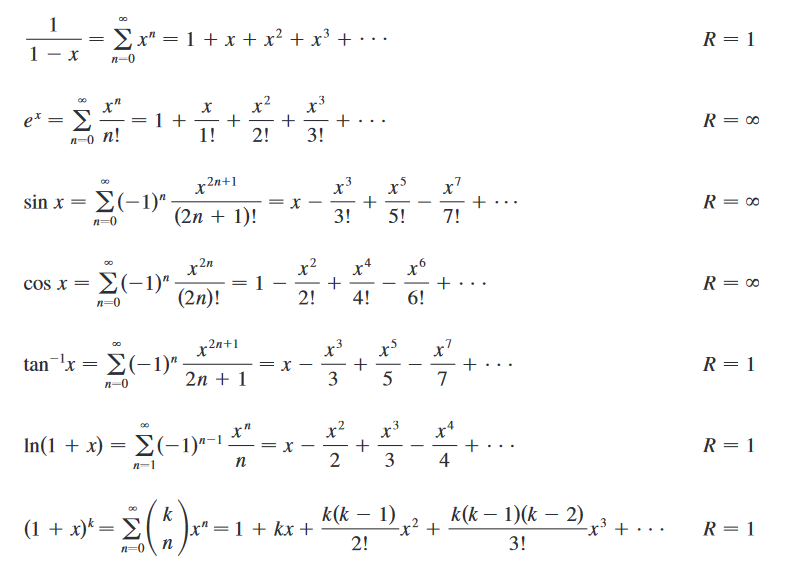
\includegraphics[scale=0.7]{table12-10}
\end{center}

\section{Applications of Taylor Polynomials}

\subsection*{Approximating Functions by Polynomails}

\subsection*{Example}
\begin{enumerate}[(a)]
    \item Approximate the function $f(x)=\sqrt[3]{x}$ by a Taylor
          polynomial of degree 2 at $a=8$.
    \item How accurate is this approximation when $7\leq x \leq 9$?
\end{enumerate}

\subsection*{Solution}
(a)
\begin{center}
    $\begin{array}{ll}
            f(x)=x^{1/3}                & f(8)=2               \\
            f'(x)=\frac{1}{3}x^{-2/3}   & f'(8)=\frac{1}{12}   \\
            f''(x)=-\frac{2}{9}x^{-5/3} & f''(8)=\frac{1}{144} \\
            f'''(x)=\frac{10}{27}x^{-8/3}
        \end{array}$
\end{center}
Using the second-degree Taylor polynomial, $T_2(x)$, the desired approximation is
$$ \sqrt[3]{x} \approx T_2(x) = 2+\frac{1}{12}(x-8)-\frac{1}{288}(x-8)^2 $$
(b) The tailor series is not alternating when $x<8$, so we can't use the Alternating
Series Estimation Theorem. But we can use the Taylor's Inequality with $n=2$ and $a=8$:
$$ |R_2(x)| \leq \frac{M}{3!}|x-8|^3 $$
where $|f'''(x)|\leq M$. Because $x \geq 7$, we have $x^{8/3} \geq 7^{8/3}$ and so
$$ f'''(x)=\frac{10}{27} \cdot \frac{1}{x^{8/3}} \leq \frac{10}{27} \cdot \frac{1}{7^{8/3}}<0.0021$$
Thereform we can take $M=0.0021$. Also $7\leq x\leq 9$, so $-1\leq x-8\leq 1$ and
$|x-8|\leq 1$. Then Taylor's Inequality gives
$$ |R_2(x)| \leq \frac{0.0021}{3!} \cdot 1^3=\frac{0.0021}{6} < 0.0004 $$
Thus, if $7\leq x\leq 9$, the approximation in part (a) is accurate within 0.0004.
\chapter{Vectors and Geometry of Space}

\section{Three-Dimensional Coordinate Systems}

\subsection*{3D Space}
The direction of the $z$-axis is determined by the \textbf{right-hand rule}.
if you curl the fingers of your right hand around the $z$-axis, in the clockwise direction
from the $x$-axis to the $y$-axis, your thumb points in the direction of the $z$-axis.

The Cartesian product $\mathbb{R}\times\mathbb{R}\times\mathbb{R}=
    \{x,y,z\} | x,y,z \in \mathbb{R}$ is the set of all ordered triples of real numbers
and is denoted by $\mathbb{R}^3$.

\subsection*{Surfaces}
In three-dimensions, an equation in $x,y,z$ represents a \emph{surface} in $\mathbb{R}^3$.

\subsection*{Example}
What surfaces in $\mathbb{R}^3$ are represented by the following equations?
\begin{enumerate}[(a)]
    \item $z=3$
    \item $y=5$
\end{enumerate}
\subsection*{Solution}
(a) $z=3$ represents the set $\{x,y,z | z=3\}$, which all the points in
$\mathbb{R}^3$ whose $z$-coordinate is 3. This is a horizontal plane parallel
to the $xy$-plane and three units above it. \\
(b) $y=5$ represents a vertical plane parallel to the $xz$-plane and five units
to the right of it.

\textbf{Distance Formula in Three Dimensions} \\
The distance $|P_1P_2|$ between the points $P_1(x_1,y_1,z_1)$ and $P_2(x_2,y_2,z_2)$ is
$$|P_1P_2|=\sqrt{(x_2-x_1)^2+(y_2-y_1)^2+(z_2-z_1)^2}$$

\textbf{Equation of a Sphere} \\
An equation of a sphere with center $C(h,k,l)$ and radius $r$ is
$$ (x-h)^2+(y-k)^2+(z-l)^2=r^2 $$
If the center is the origin $O$, then the equation is
$$ x^2+y^2+z^2=r^2 $$

\subsection*{Example}
What region in $\mathbb{R}^3$ is represents by the following inequalities?
$$1\leq x^2+y^2+z^2\leq 4 \qquad z\leq 0$$
\subsection*{Solution}
The inequalities can be rewritten as
$$1\leq \sqrt{x^2+y^2+z^2}\leq 2$$
so they represent the points $(x,y,z)$ whose distance from the origin is at least 1 and at most 2.
\begin{center}
    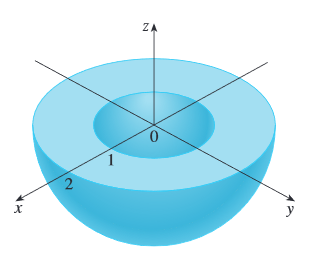
\includegraphics[scale=0.7]{example13-1}
\end{center}

\section{Vectors}

\subsection*{Combining Vectors}
\textbf{Definition of Vector Addition} \\
If \textbf{u} and \textbf{v} are vectors positioned
so the intial point of \textbf{v} is at the terminal point of \textbf{u}, then
the sum \textbf{u + v} is the vector from the initial point of \textbf{u}
to the terminal point of \textbf{v}.
\begin{center}
    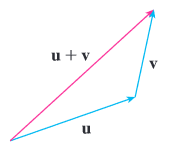
\includegraphics[scale=0.7]{example13-2-1}
\end{center}

\textbf{Definition of Scalar Multiplication} \\
If $c$ is scalar and \textbf{v} is a vector, then the \textbf{scalar multiple}
$c\mathbf{v}$ is the vector whose length is $|c|$ times the length of
\textbf{v} and whose direction is the same as \textbf{v} if $c>0$ and
is opposite to \textbf{v} if $c<0$.
\begin{center}
    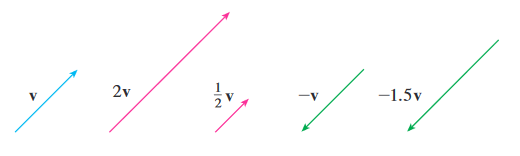
\includegraphics[scale=0.7]{example13-2-2}
\end{center}

\subsection*{Components}
The \textbf{components} of vector \textbf{a} are written as
$$\mathbf{a}=\ev{a_1,a_2} \qquad \mathbf{a}=\ev{a_1,a_2,a_3}$$

\subsection*{Example}
Find the vector represented by the directed line segment with initial
point $A(2,-3,4)$ and terminal point $B(-2,1,1)$.

\subsection*{Solution}
$$\mathbf{a}=\ev{x_2-x_1,y_2-y_1,z_2-z_1}$$
$$\mathbf{a}=\ev{-2-2,1-(-3),1-4}=\ev{-4,4,-3}$$

\subsection*{Example}
If \textbf{a}=$\ev{4,0,3}$, find $|\textbf{a}|$.

\subsection*{Solution}
$$|\textbf{a}|=\sqrt{4^2+0^2+3^2}=\sqrt{25}=5$$

\subsection*{Properties of Vectors}
If \textbf{a}, \textbf{b}, and \textbf{c} are vectors in $V_n$ and $c$ and $d$ are scalars
\begin{multicols}{2}
    \begin{enumerate}
        \item $\textbf{a+b=b+a}$
        \item $\textbf{a+(b+c)=(a+b)+c}$
        \item $\textbf{a+0=a}$
        \item $\textbf{a+(-a)=0}$
        \item $c\textbf{(a+b)}=c\textbf{a}+c\textbf{b}$
        \item $(c+d)\textbf{a}=c\textbf{a}+d\textbf{a}$
        \item $(cd)\textbf{a}=c(d\textbf{a})$
        \item $1\textbf{a}=\textbf{a}$
    \end{enumerate}
\end{multicols}

\textbf{Standard Basis Vectors}
$$ \textbf{i}=\ev{1,0,0} \qquad \textbf{j}=\ev{0,1,0} \qquad \textbf{k}=\ev{0,0,1} $$

\subsection*{Example}
Find the unit vector in the direction of the vector $2\textbf{i}-\textbf{k}-2\textbf{k}$.

\subsection*{Solution}
The given vector has length
$$|2\textbf{i}-\textbf{k}-2\textbf{k}|=\sqrt{2^2+(-1)^2+(-2)^2}=\sqrt{9}=3$$
and by the equation $\textbf{u}=\cfrac{1}{|\textbf{a}|}\textbf{a}=\cfrac{\textbf{a}}{|\textbf{a}|}$,
the unit vector is
$$\frac{1}{3}(2\textbf{i}-\textbf{j}-2\textbf{k})=\frac{2}{3}\textbf{i}-
    \frac{1}{3}\textbf{j}-\frac{2}{3}\textbf{k}$$

\section{The Dot Product}

\subsection*{Definition}
If $\textbf{a}=\ev{a_1,a_2,a_3}$ and $\textbf{b}=\ev{b_1,b_2,b_3}$, then the
\textbf{dot product} of \textbf{a} and \textbf{b} is
$$\mathbf{a\cdot b}=a_1 b_1+a_2 b_2+a_3 b_3$$

\subsection*{Properties of the Dot Product}
If \textbf{a}, \textbf{b}, and \textbf{c} are vectors in $V_3$ and $c$ is scalar
\begin{multicols}{2}
    \begin{enumerate}
        \item $\mathbf{a\cdot a=|a|^2}$
        \item $\mathbf{a\cdot b=b\cdot a}$
        \item $\mathbf{a\cdot (b\cdot c)=a\cdot b+a\cdot c}$
        \item $(c\mathbf{a})\cdot\mathbf{b}=c(\mathbf{a\cdot b})=\mathbf{a}\cdot(c\mathbf{b})$
        \item $\mathbf{0\cdot a}=0$
        \item []
    \end{enumerate}
\end{multicols}

\subsection*{Theorem}
If $\theta$ is the angle between the vectors \textbf{a} and \textbf{b}, then
$$\mathbf{a\cdot b} = \mathbf{|a||b|}\:cos\:\theta$$

Two nonzero vectors are \textbf{perpendicular} or \textbf{orthogonal} if the angle
between then is $\theta=\pi/2$. The dot product gives
$$\mathbf{a\cdot b}=\mathbf{|a||b|}\:cos(\pi/2)=0$$
Two vectors \textbf{a} and \textbf{b} are orthogonal if and only if $\mathbf{a\cdot b}=0$.

\subsection*{Projections}
Scalar projection of \textbf{b} onto \textbf{a}: $\qquad comp_a\textbf{b}=
    \mathbf{\cfrac{a\cdot b}{|a|}}$ \\
Vector projection of \textbf{b} onto \textbf{a}: $\qquad proj_a\textbf{b}=
    \mathbf{\left(\cfrac{a\cdot b}{|a|}\right)\cfrac{a}{|a|}}=\mathbf{\cfrac{a\cdot b}{|a|^2}a}$

\subsection*{Example}
Find the scalar projection and vector projection of $\textbf{b}=\ev{1,1,2}$ onto
$\textbf{a}=\ev{-2,3,1}$.

\subsection*{Solution}
Since $|\textbf{a}|=\sqrt{(-2)^2+3^2+1^2}=\sqrt{14}$, the scalar projection of \textbf{b}
onto \textbf{a} is:
$$comp_a\textbf{b}=\mathbf{\frac{a\cdot b}{|a|}}=\frac{(-2)(1)+3(1)+1(2)}{\sqrt{14}}=\frac{3}{\sqrt{14}}$$
The vector projection is this scalar projection times the unit vector in the direction of \textbf{a}:
$$proj_a\textbf{b}=\frac{3}{\sqrt{14}}\mathbf{\frac{a}{|a|}}=\frac{3}{14}\textbf{a}=
    \ev{-\frac{3}{7},\frac{9}{14},\frac{3}{14}}$$

\section{The Cross Product}

\subsection*{Definition}
If $\textbf{a}=\ev{a_1,a_2,a_3}$ and $\textbf{b}=\ev{b_1,b_2,b_3}$, then the
\textbf{cross product} of \textbf{a} and \textbf{b} is the vector
$$\mathbf{a \times b}=\ev{a_2b_3-a_3b_2,a_3b_1-a_1b_3,a_1b_2-a_2b_1}$$
This Definition can be rewritten using second-order determinants and the standard
basis vectors \textbf{i, j,} and \textbf{k}
$$\mathbf{a\times b}=\
    \begin{vmatrix}
        \textbf{i} & \textbf{j} & \textbf{k} \\
        a_1        & a_2        & a_3        \\
        b_1        & b_2        & b_3
    \end{vmatrix}$$


\subsection*{Example}
If $\textbf{a}=\ev{1,3,4}$ and $\textbf{b}=\ev{2,7,-5}$, then
\begin{align*}
    \mathbf{a\times b} & =\
    \begin{vmatrix}
        \textbf{i} & \textbf{j} & \textbf{k} \\
        1          & 3          & 4          \\
        2          & 7          & -5
    \end{vmatrix}                                                                                                               \\
                       & =\begin{vmatrix}
        3 & 4  \\
        7 & -5
    \end{vmatrix}\textbf{i} - \begin{vmatrix}
        1 & 4  \\
        2 & -5
    \end{vmatrix}\textbf{j} + \begin{vmatrix}
        1 & 3 \\
        2 & 7
    \end{vmatrix}\textbf{k} \\
                       & =(-15-28)\textbf{i}-(-5-8)\textbf{j}+(7-6)\textbf{k}=-43\textbf{i}+13\textbf{j}+\textbf{k}
\end{align*}


\subsection*{Theorem}
The vector $\mathbf{a\times b}$ is orthogonal to both \textbf{a} and \textbf{b}.

\subsubsection*{Proof} $\mathbf{(a\times b)\cdot b}=0$. Therefore $\mathbf{a\times b}$
is orthogonal to both \textbf{a} and \textbf{b}.

\subsection*{Theorem}
If $\theta$ is the angle between \textbf{a} and \textbf{b} (so $0\leq \theta \leq \pi$), then
$$|\mathbf{a\times b}|=\mathbf{|a||b|}\:sin\:\theta$$

\subsection*{Corollary}
Two nonzero vectors \textbf{a} and \textbf{b} are parallel if and only if
$$\mathbf{a\times b=0}$$

\subsection*{Example}
Find the vector perpendicular to the plane that passes through the points $P(1,4,6)$,
$Q(-2,5,-1)$, and $R(1,-1,1)$.

\subsection*{Solution}
\begin{enumerate}
    \item[] $\overrightarrow{PQ}=(-2-1)\textbf{i}+(5-4)\textbf{j}+(-1-6)\textbf{k}=\mathbf{-3i+j-7k}$
    \item[] $\overrightarrow{PR}=(1-1)\textbf{i}+(-1-4)\textbf{j}+(1-6)\textbf{k}=\mathbf{-5j-5k}$
\end{enumerate}
We compute the cross product of these vectors:
$$\overrightarrow{PQ}\times \overrightarrow{PR}=\begin{vmatrix}
        \textbf{i} & \textbf{j} & \textbf{k} \\
        -3         & 1          & -7         \\
        0          & -5         & -5
    \end{vmatrix}=-40\textbf{i}-15\textbf{j}+15\textbf{k}$$

\subsection*{Properties of the Cross Product}
If \textbf{a, b,} and \textbf{c} are vectors and $c$ is a scalar, then
\begin{enumerate}
    \item $\mathbf{a\times b=-b\times a}$
    \item $(c\textbf{a})\times \textbf{b}=c(\mathbf{a\times b})=\textbf{a}\times(c\textbf{b})$
    \item $\mathbf{a\times (b+c)=a\times b+a\times c}$
    \item $\mathbf{(a+b)\times c=a\times c+b\times c}$
    \item $\mathbf{a\cdot (b\times c)=(a\times b)\cdot c}$
    \item $\mathbf{a\times (b\times c)=(a\cdot c)b-(a\cdot b)c}$
\end{enumerate}

\subsection*{Triple Products}
The volume of the parallelepiped determined by the vectors \textbf{a, b,} and \textbf{c}
is the magnitude of their scalar triple product:
$$V=|\mathbf{a\cdot (b\times c)}|=\begin{vmatrix}
        a_1 & a_2 & a_3 \\
        b_1 & b_2 & b_3 \\
        c_1 & c_2 & c_3
    \end{vmatrix}$$
When the volume is 0, the vectors lie in the same plane and are \textbf{coplanar}.

\section{Equations of Lines and Planes}

\subsection*{Lines}

$$\textbf{r}=\textbf{r}_0|t\textbf{v}$$
is the \textbf{vector equation} of $L$. Each value of the \textbf{parameter} $t$ gives
the position vector \textbf{r} of a point on $L$. We can also write $\textbf{r}=\ev{x,y,z}$
and $\textbf{r}_0=\ev{x_0,y_0,z_0}$, so the vector equation becomes
$$\ev{x,y,z}=\ev{x_0+ta,y_0+tb,z_0+tc}$$

\subsection*{Example}
Find a vector equation and parametric equations for the line that passes through the point
$(5,1,3)$ and is parallel to the vector $\textbf{i}+4\textbf{j}-2\textbf{k}$.

\subsection*{Solution}
Here $\textbf{r}_0=\ev{5,1,3}=5\textbf{i}+\textbf{j}+3\textbf{k}$ and
$\textbf{v}=\textbf{i}+4\textbf{j}-2\textbf{k}$, so the vector equation becomes
\begin{enumerate}
    \item[] $\textbf{r}=(5\textbf{i}+\textbf{j}+3\textbf{k})+t(\textbf{i}+4\textbf{j}-2\textbf{k})$
    \item[] $\textbf{r}=(5+t)\textbf{i}+(1+4t)\textbf{j}+(3-2t)\textbf{k}$
\end{enumerate}
Parametric equations are
$$x=5+t \qquad y=1+4t \qquad z=3-2t$$

\subsection*{Planes}

$$\textbf{n}\cdot (\textbf{r}-\textbf{r}_0=0)$$
which can be rewritten as
$$\mathbf{n\cdot r}=\textbf{n}\cdot \textbf{r}_0$$
Either of the two equations are the \textbf{vector equation of the plane}.

A \textbf{scalar equation of the plane} through point $P_0(x_0,y_0,z_0)$ with normal
vector $\textbf{n}=\ev{a,b,c}$ is
$$a(x-x_0)+b(y-y_0)+c(z-z_0)=0$$
which can be rewritten as
$$ax+by+cz+d=0$$
where $d=-(ax_0+by_0+cz_0)$.

\subsection*{Example}
Find an equation of the plane that passes through the points $P(1,3,2)$, \newline
$Q(3,-1,6)$, and $R(5,2,0)$.

\subsection*{Solution}
The vectors \textbf{a} and \textbf{b} corresponding to $\overrightarrow{PQ}$ and
$\overrightarrow{PR}$ are
$$\textbf{a}=\ev{2,-4,4} \qquad \textbf{b}=\ev{4,-1,-2}$$
Since both \textbf{a} and \textbf{b} lie in the plane, their cross product $\mathbf{a\times b}$
is orthogonal to the plane and can be taken as the normal vector. Thus
$$\mathbf{n=a\times b}=\begin{vmatrix}
        \textbf{i} & \textbf{j} & \textbf{k} \\
        2          & -4         & 4          \\
        4          & -1         & -2
    \end{vmatrix}=12\textbf{i}+20\textbf{j}+14\textbf{k}$$
With the point $P(1,3,2)$ and the normal vector \textbf{n}, an equation of the plane is
$$12(x-1)+20(y-3)+14(z-2)=0$$
or
$$6x+10y+7z=50$$

\subsection*{Distances}
The formula for the distance $D$ can be written as
$$D=\frac{|ax_1+by_1+cz_1+d|}{\sqrt{a^2+b^2+c^2}}$$

\subsection*{Example}
Find the distance between the parallel planes $10x+2y-2z-5$ and $5x+y-z=1$

\subsection*{Solution}
The planes are parallel because their normal vectors $\ev{10,2,-2}$ and
$\ev{5,1,-1}$ are parallel. To find the distance between the planes, we choose
any point on one plane and calculate its distance to the other plane. If we
plug in $y=z=0$ into the first equation, we get $10x=5$ and so $(\frac{1}{2},0,0)$
is a point in the plane.
$$D=\frac{|5(\frac{1}{2})+1(0)-1(0)-1|}{\sqrt{5^2+1^2+(-1)^2}}=\frac{\frac{3}{2}}{3\sqrt{3}}
    =\frac{\sqrt{3}}{6}$$

\section{Cylinders and Quadric Surfaces}

\subsection*{Cylinders}
A \textbf{cylinder} is a surface that consists of all lines that are parallel to a
given line and pass through a given plane curve.

\subsection*{Quadric Surfaces}
A \textbf{quadric surface} is the graph of a second-degree equation in three variables
$x$, $y$, and $z$. The most general such equation is
$$Ax^2+By^2+Cz^2+Dxy+Eyz+Fxz+Gx+Hy+Iz+J=0$$
where $A, B, C, \dots , J$ are constants, but by translation and rotation it can be
brought into one of the two standard forms
$$Ax^2+By^2+Cz^2+J=0 \qquad Ax^2+By^2+Iz=0$$

\subsection*{Graphs of Quadric Surfaces}
\begin{center}
    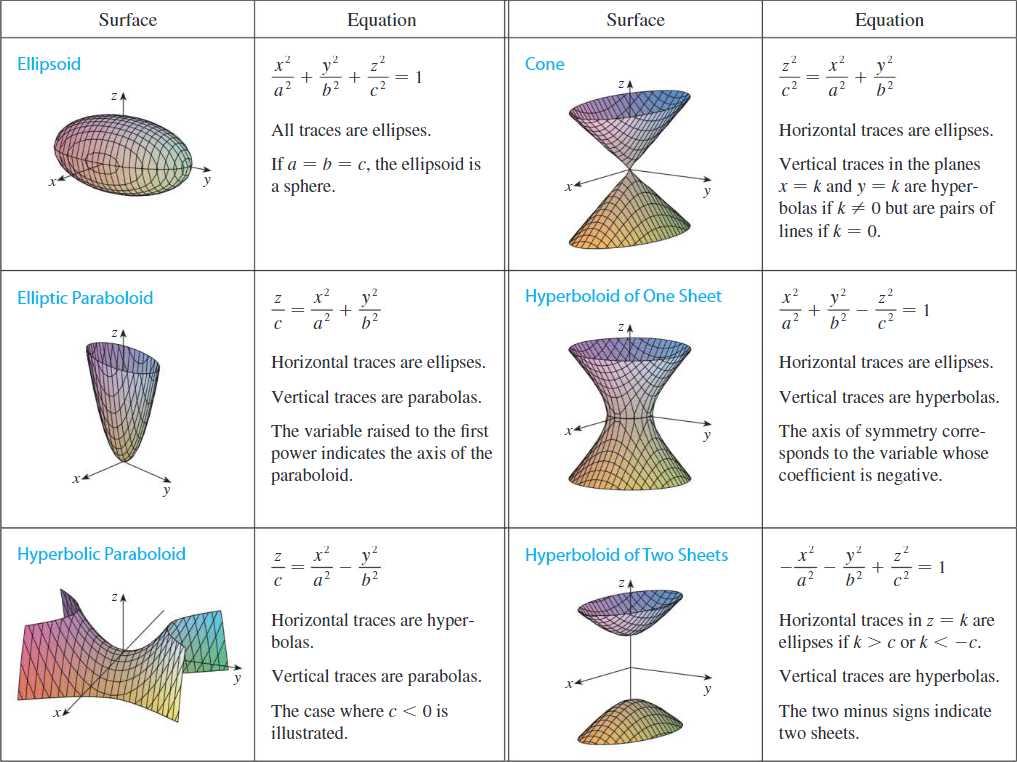
\includegraphics[width=\linewidth]{table13-6.png}
\end{center}
\chapter{Vector Functions}

\section{Vector Functions and Space Curves}
A vector expression of the form $\ev{f(t),g(t),h(t)}$ is called a vector function.
It can also be described as three separate functions, $x=f(t)$, $y=g(t)$, and $z=h(t)$,
that describe points in space. In this case, we refer to the set of equations as
parametric equations for the curve.
$$r(t)=\ev{f(t),g(t),h(t)}=f(t)\ihat+g(t)\jhat+h(t)\khat$$

\subsection*{Example}
Describe the curves $\ev{cos\:t,sin\:t,0}$, $\ev{cos\:t,sin\:t,t}$, and
$\ev{cos\:t,sin\:t,2t}$

\subsection*{Solution}
As $t$ varies, the first two coordinates in all three functions trace out a unit circle.
In the first curve, the $z$-coordinate is always 0, so this is a 2D unit circle in the
$xy$ plane. In the second curve, the $z$-coordinate varies with $t$ which will
produce a helix. In the third curve, the $z$ coordinate varies twice as fast as $t$
which produces a stretched out helix. Below are the two helixes:
\begin{center}
    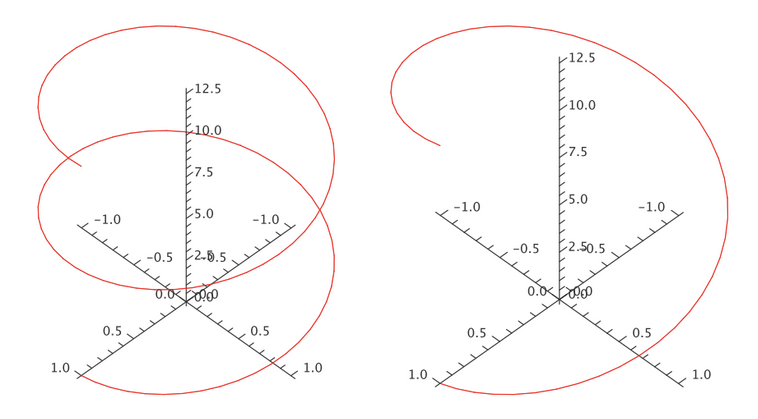
\includegraphics[scale=0.5]{example14-1-1.png}
\end{center}

If $r(t)=\ev{f(t),g(t),h(t)}$, then
$$\lim_{t\to a}r(t)=\ev{\lim_{t\to a}f(t),\lim_{t\to a}g(t),\lim_{t\to a}h(t)}$$
provided the limits of the component functions exist.

\subsection*{Example}
Graph the projections of $\ev{cos\:t,sin\:t,2t}$ onto the $xz$ plane and the $yz$ plane

\subsection*{Solution}
The 2D vector function for the projection onto the $xz$ plane is $\ev{cos\:t,2t}$,
or in parametric force: $x=cos\:t$, $z=2t$. By substituting for $t$, we get
$x=cos(z/2)$, which is the curve below on the left. For the projection onto the $yz$
plane, we start with the vector function $\ev{sin\:t,2t}$, which is $y=sin\:t$,
$z=2t$. Substituting for $t$ gives $y=sin(z/2)$ as shown below on the right.
\begin{center}
    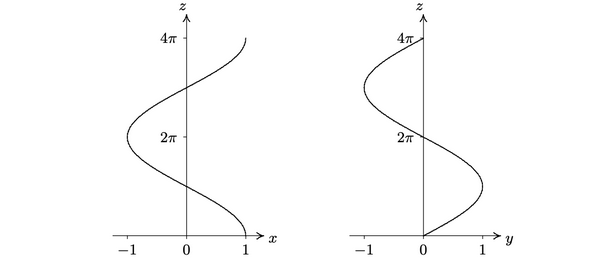
\includegraphics[scale=0.8]{example14-1-2.png}
\end{center}

\section{Derivatives and Integrals of Vector Functions}

\subsection*{Derivatives}
The derivative of a vector function is defined the same way as for real-valued functions:
$$\dv{r}{t}=r'(t)=\lim_{h\to 0}\frac{r(t+h)-r(t)}{h}$$
If $r(t)=\ev{f(t),g(t),h(t)}=f(t)\ihat+g(t)\jhat+h(t)\khat$ where $f$, $g$, and $h$
are differentiable functions, then
$$r'(t)=\ev{f'(t),g'(t),h'(t)}=f'(t)\ihat+g'(t)\jhat+h'(t)\khat$$

\subsection*{Example}
\begin{enumerate}[(a)]
    \item Find the derivative of $r(t)=(1+t^3)\ihat+te^{-t}\jhat+sin\:2t\khat$
    \item Find the unit tangent vector at the point where $t=0$
\end{enumerate}

\subsection*{Solution}
\begin{enumerate}[(a)]
    \item $r'(t)=3t^2\ihat+(1-t)e^{-t}\jhat+2cos\:2t\khat$
    \item Since $r(0)=\ihat$ and $r'(0)=\jhat+2\khat$, the unit tangent vector at
          (1,0,0) is $$T(0)=\frac{r'(0)}{|r'(0)|}=\frac{\jhat+2\khat}{\sqrt{1+4}}=
              \frac{1}{\sqrt{5}}\jhat+\frac{2}{\sqrt{5}}\khat$$
\end{enumerate}

\subsection*{Theorem}
Suppose \textbf{u} and \textbf{v} are differentiable vector functions, $c$ is a scalar,
and $f$ is a real-valued function. Then
\begin{center}
    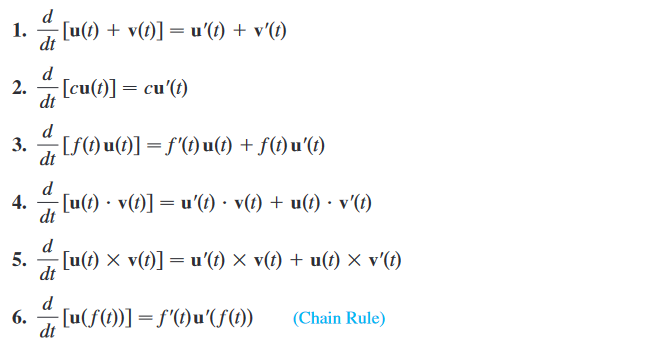
\includegraphics[scale=0.8]{example14-2-1.png}
\end{center}

\subsection*{Integrals}
$$\int_a^b\textbf{r}(t)\:dt=\left(\int_a^bf(t)\:dt\right)\ihat+\left(\int_a^bg(t)\:dt\right)
    \jhat+\left(\int_a^bh(t)\:dt\right)\khat$$

\subsection*{Example}
If $\textbf{r}(t)=2cos\:t\ihat+sin\:t\jhat+2t\khat$, then
\begin{align*}
    \int\textbf{r}(t)\:dt & =\left(\int 2cos\:t\:dt\right)\ihat+\left(\int cos\:t\:dt\right)\jhat+\left(\int 2t\:dt\right)\khat \\
                          & =2sin\:t\ihat-cos\:t\jhat+t^2\khat+C
\end{align*}
Where $C$ is a vector constant of integration, and
$$\int_0^{\pi/2}\textbf{r}(t)\:dt=\left[2sin\:t\ihat-cos\:t\jhat+t^2\khat\right]_0^{\pi/2}=
    2\ihat+\jhat+\frac{\pi^2}{4}\khat$$

\section{Arc Length and Curvature}

\subsection*{Length of a Curve}
$$L=\int_a^b\sqrt{[f'(t)]^2+[g'(t)]^2+[h'(t)]^2}\:dt$$
$$=\int_a^b\sqrt{(\dv{x}{t})^2+(\dv{y}{t})^2+(\dv{z}{t})^2}\:dt$$
The formula can be put into the compact form $L=\int_a^b|\textbf{r}'(t)|\:dt$

\subsection*{Example}
Find the length of the arc of the circular helix with vector equation
$\textbf{r}(t)=\cos{t}\ihat+\sin{t}\jhat+t\khat$ from the point $(1,0,0)$ to the
point $(1,0,2\pi)$

\subsection*{Solution}
Since $\textbf{r}'(t)=-\sin{t}\ihat+\cos{t}\jhat+\khat$, we have
$$|\textbf{r}'(t)|=\sqrt{(-\sin{t})^2+cos^2t+1}=\sqrt{2}$$
The arc from (1,0,0) to (1,0,$2\pi$) is described by the parameter interval
$0\leq t\leq 2\pi$ and so we have
$$L=\int_0^{2\pi}|\textbf{r}'(t)|\:dt=\int_0^{2\pi}\sqrt{2}\:dt=2\sqrt{2}\pi$$

\subsection*{Proof}
$$\kappa=\left|\dv{\textbf{T}}{s}\right|\to\dv{\textbf{T}}{t}=
    \dv{\textbf{T}}{s}\dv{s}{t}$$
$$\kappa=\frac{|d\textbf{T}/dt|}{|ds/dt|}$$
$$\kappa(t)=\frac{|\textbf{T}'(t)|}{|\textbf{r}'(t)|}
    =\frac{|\textbf{r}'(t)\times\textbf{r}''(t)|}{|\textbf{r}'(t)|^3}$$

We summarize here the formulas for unit tangent, unit normal and binormal vectors,
and curvature.
$$\textbf{T}(t)=\frac{\textbf{r}'(t)}{|\textbf{r}'(t)|} \qquad
    \textbf{N}(t)=\frac{\textbf{T}'(t)}{|\textbf{T}'(t)|} \qquad
    \textbf{B}(t)=\textbf{T}(t)\times\textbf{N}(t)$$
$$\kappa=|\dv{\textbf{T}}{s}|=\frac{|\textbf{T}'(t)|}{|\textbf{r}'(t)|}
    =\frac{|\textbf{r}'(t)\times\textbf{r}''(t)|}{|\textbf{r}'(t)|^3}$$

\section{Motion in Space: Velocity and Acceleration}
Suppose a particle moves through space so that its position vector at time $t$ is
$\textbf{r}(t)$. Notice that for small values of $h$, the vector
$$\frac{\textbf{r}(t+h)-\textbf{r}(t)}{h}$$
approximates the direction of the particle moving along the curve $\textbf{r}(t)$.
Its magnitude measures the size of the displacement vector per unit time. The vector
gives the average velocity over a time interval of length and its limit is the
\textbf{velocity vector} $\textbf{v}(t)$ at time $t$:
$$\textbf{v}(t)=\lim_{h\to 0}\frac{\textbf{r}(t+h)-\textbf{r}(t)}{h}=\textbf{r}'(t)$$

\subsection*{Example}
The position vector of an object moving in a place is given by $\textbf{r}(t)=
    t^3\ihat+t^2\jhat$. Find its velocity, speed, and acceleration when $t=1$.

\subsection*{Solution}
The velocity and acceleration equations at time $t$ are
$$\textbf{v}(t)=\textbf{r}'(t)=3t^2\ihat+2t\jhat$$
$$\textbf{a}(t)=\textbf{r}''(t)=6t\ihat+2\jhat$$
and the speed is
$$|\textbf{v}(t)|=\sqrt{(3t^2)^2+(2t)^2}=\sqrt{9t^4+4t^2}$$
When $t=1$, we have
$$\textbf{v}(1)=3\ihat+2\jhat\qquad\textbf{a}(1)=6\ihat+2\jhat\qquad|\textbf{v}(1)|=\sqrt{13}$$

\subsection*{Parametric Equations of Trajectory}
$$x=(v_0\cos{\alpha})t\qquad y=(v_0\sin{\alpha})t=\frac{1}{2}gt^2$$

\subsection*{Tangential and Normal Components of Acceleration}
$$\textbf{T}(t)=\frac{\textbf{v}}{v} \qquad \textbf{v}=v\textbf{T}$$
$$\textbf{a}=\textbf{v}'=v'\textbf{T}+v\textbf{T}'$$
$$\kappa=\mathbf{\cfrac{|T'|}{|r'|}}=\cfrac{|\textbf{T}'|}{v} \qquad
    |\textbf{T}'|=\kappa v$$
$$\textbf{N}=\mathbf{\frac{T'}{|T'|}}\qquad \mathbf{T'=|T'|N=\kappa}v\textbf{N}$$
$$\textbf{a}=v'\textbf{T}+\kappa v^2 \textbf{N}$$

\subsection*{Keplar's Laws}
\begin{enumerate}
    \item A planet revolves around the Sun in an elliptical orbit with the Sun at one focus.
    \item The line joining the Sun to a planet sweeps out equal areas in equal times.
    \item The square of the period of revolution of a planet is proportional to the cube
          of the length of the major axis of its orbit.
\end{enumerate}
\chapter{Partial Derivatives}

\section{Functions of Several Variables}
A function $f$ of two variables is a rule that assigns to each ordered pair of
real numbers $(x,y)$ in a set $D$ a unique real number denoted by
$f(x,y)$. The set $D$ is the \textbf{domain} of $f$ and its \textbf{range} is
the set of values that takes on, that is, ${f(x,y)\:|\:(x,y)\in D}$.

\subsection*{Example}
Find the domains of the following functions and evaluate $f(3,2)$
\begin{enumerate}[(a)]
    \item $f(x,y)=\cfrac{\sqrt{x+y+1}}{x-1}$
    \item $f(x,y)=x\ln(y^2-x)$
\end{enumerate}

\subsection*{Solution}
\begin{enumerate}[(a)]
    \item $$f(3,2)==\frac{\sqrt{3+2+1}}{3-1}\frac{\sqrt{6}}{2}$$
          The expression for $f$ makes sense if the denominator is not 0 and the
          quantity under the square root sign is nonnegative. So the domain of $f$ is
          $$D=\{(x,y)\:|\:x+y+1\geq 0, x\neq 1\}$$
          The inequality $x+y+1\geq 0$ describes the points that lie on or above the line
          $y=-x-1$, while $x\neq 1$ means that the point on the line $x=1$ must be excluded
          from the domain
    \item $$f(3,2)=3\ln(2^2-3)=3\ln(1)=0$$
          Since $\ln(y^2-x)$ is defined only when $y^2-x>0$ that is, $x<y^2$, the
          domain of $f$ is $D=\{(x,y)\:|\:x<y^2\}$. This is the set of points on the left
          of the parabola $x=y^2$.
\end{enumerate}

\subsection*{Definition}
If $f$ is a function of two variables with domain $D$, then the graph of $f$ is the
set of all points $(x,y,z)$ in $\mathbb{R}^3$ such that $z=f(x,y)$ and $(x,y)$ is in $D$

\subsection*{Example}
Sketch the graph of the function $f(x, y) = 6 - 3x - 2y$

\subsection*{Solution}
The graph of $f$ has the equation $z = 6 - 3x - 2y$, or $3x + 2y + z = 6$, which represents
a plane. To graph the plane we first find the intercepts. Putting $y = z = 0$ in the
equation, we get $x = 2$ as the $x$-intercept. Similarly, the $y$-intercept is 3 and the
$z$-intercept is 6. This helps us sketch the portion of the graph that lies in the
first octant.
\begin{center}
    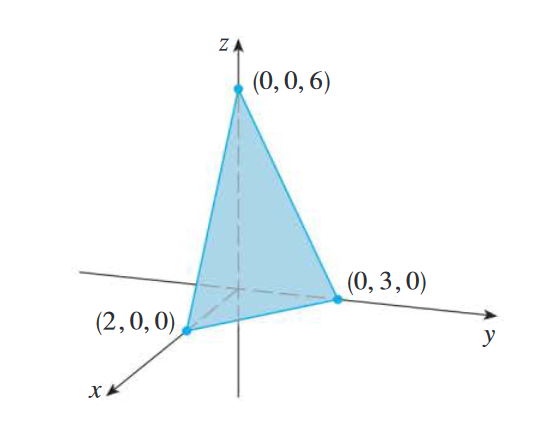
\includegraphics[scale=0.6]{example15-1-1.png}
\end{center}

\subsection*{Definition}
The level curves of a function $f$ of two variables are the curves with the equations
$f(x,y)=k$, where $k$ is a constant in the range of $f$.

\subsection*{Example}
Sketch the level curves of the function $f(x,y)=6-3x-2y$ for the values $k=-6,0,6,12$

\subsection*{Solution}
The level curves are
$$6-3x-2y=k \qquad \text{or} \qquad 3x+2y+(k-6)=0$$
This is a family of lines with slope $-\frac{3}{2}$. The four particular level curves
with $k=-6,0,6,12$ are $3x+2y-12=0$, $3x+2y-6=0$, $3x+2y=0$, and $3x+2y+6=0$. They're
equally spaced because the graph of $f$ is a plane.
\begin{center}
    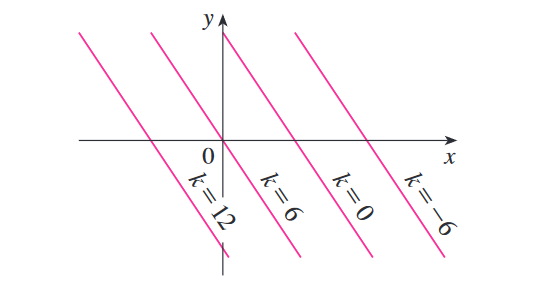
\includegraphics[scale=0.7]{example15-1-2.png}
\end{center}

\subsection*{Functions of Three or More Variables}
A \textbf{function of three variables}, $f$, is a rule that assigns to each ordered triple
$(x, y, z)$ in a domain $D\subset\mathbb{R}^3$ unique real number denoted by $f(x, y, z)$. For instance,
the temperature $T$ at a point on the surface of the Earth depends on the longitude $x$
nd the latitude y of the point and on the time $t$, so we could write $T = f(x, y, t)$.

\section{Limits and Continuity}

\subsection*{Definition}
Let $f$ be a function of two variables whose domain $D$ includes points arbitrarily
close to $(a, b)$. Then we say that the limit of $f(x, y)$ as $(x, y)$ approaches
$(a, b)$ is $L$ and we write
$$\lim_{(x,y)\to(a,b)}f(x,y)=L$$
If for every number $\epsilon>0$ there is a corresponding number $\sigma>0$ such that
if $(x,y)\in D$ and $0<\sqrt{(x-a)^2+(y-b)^2}<\delta$ and $|f(x, y) - L| < \epsilon$

\subsection*{Example}
Show that $\displaystyle\lim_{(x,y)\to(0,0)}\cfrac{x^2-y^2}{x^2+y^2}$ does not exist.

\subsection*{Solution}
Let $f(x,y)=(x^2-y^2)/(x^2+y^2)$. First let's approach (0,0) along the $x$-axis.
Then $y=0$ gives $f(x,0)=x^2/x^2=1$ for all $x\neq 0$, so
$$f(x,y)\to 1 \qquad \text{as} \qquad (x,y)\to(0,0)\quad\text{along the x-axis}$$
We now approach along the $y$-axis by putting $x=0$. Then $f(0,y)=\cfrac{-y^2}{y^2}=-1$
for all $y\neq 0$, so
$$f(x,y)\to -1 \qquad \text{as} \qquad (x,y)\to(0,0)\quad\text{along the y-axis}$$
Since $f$ has two different limits along two different lines, the limit does not exist.

\subsection*{Definition}
A function $f$ of two variables is called continuous at $(a,b)$ if
$$\lim_{(x,y)\to(a,b)} f(x,y)=f(a,b)$$
We say $f$ is continuous on $D$ if $f$ is continuous at every point $(a, b)$ in $D$.

\subsection*{Example}
Evaluate $\displaystyle\lim_{(x,y)\to(1,2)}(x^2y^3-x^3y^2+3x+2y)$

\subsection*{Solution}
Since $f(x,y)=(x^2y^3-x^3y^2+3x+2y)$ is a polynomial, it is continuous everywhere,
so we can find the limit through direct substitution:
$$\lim_{(x,y)\to(1,2)}(x^2y^3-x^3y^2+3x+2y)=(1)^2(2)^3-(1)^3(2)^2+(3)(1)+(2)(2)=11$$

\section{Partial Derivatives}
In general, if $f$ is a function of two variables $x$ and $y$, suppose we let only $x$
vary while keeping $y$ fixed, say $y = b$, where $b$ is a constant. Then we are really
considering a function of a single variable $x$, namely, $g(x) = f(x, b)$. If $g$ has
a derivative at $a$, then we call it the \textbf{partial derivative of $f$ with respect to $x$
    at $(a, b)$} and denote it by $f_x(a, b)$. Thus
$$f_x(a, b)=g'(a) \qquad \text{where} \qquad g(x) = f(x, b)$$
$$\text{which becomes} \qquad f_x(a,b)=\lim_{h\to 0}\frac{f(a+h,b)-f(a,b)}{h}$$
Similarly, the partial derivative of $f$ with respect to $y$ at $(a, b)$, denoted
by $f_y(a, b)$, is obtained by keeping $x$ fixed $(x = a)$ and finding the ordinary
derivative at $b$ of the function $G(y) = f(a, y)$:
$$f_y(a,b)=\lim_{h\to 0}\frac{f(a+h,b)-f(a,b)}{h}$$

\subsection*{Notations for Partial Derivatives}
If $z=f(x,y)$, we write
$$f_x(x,y)=f_x=\pdv{f}{x}=\frac{\partial}{\partial x}f(x,y)=\pdv{z}{x}=f_1=D_1f=D_xf$$
$$f_y(x,y)=f_y=\pdv{f}{y}=\frac{\partial}{\partial y}f(x,y)=\pdv{z}{y}=f_2=D_2f=D_yf$$

\subsection*{Rules for Finding Partial Derivatives of $z=f(x,y)$}
\begin{enumerate}
    \item To find $f_x$, regard $y$ as a constant and differentiate $f(x, y)$ with respect to $x$
    \item To find $f_y$, regard $x$ as a constant and differentiate $f(x, y)$ with respect to $y$
\end{enumerate}

\subsection*{Example}
If $f(x, y)  = x^3+x^2y^3-2y^2$, find $f_x(2, 1)$ and $f_y(2, 1)$

\subsection*{Solution}
Holding $y$ cosntant and differentiating with respect to $x$, we get
$$f_x(x,y)=3x^2+2xy^3$$
$$f_x(2,1)=3\cdot 2^2+2\cdot 2\cdot 1^3=16$$
Holding $x$ constant and differentiating with respect to $y$, we get
$$f_y(x,y)=3x^2y^2-4y$$
$$f_y(2,1)=3\cdot 2^2\cdot 1^2-4\cdot 1=8$$

\subsection*{Example}
Find $\partial z/\partial x$ and find $\partial z/\partial y$ if $z$ is defined implicitly
as a function $x$ and $y$ by the equation
$$x^3+y^3+z^3+6xzy=1$$

\subsection*{Solution}
To find $\partial z/\partial x$, we differentiate implicitly with respect to $x$,
being careful to treat $y$ as a constant:
$$3x^2+3z^2\pdv{z}{x}+6yz+6xy\pdv{z}{x}=0$$
Solving this equation for $\partial z/\partial x$, we obtain
$$\pdv{z}{x}=-\frac{x^2+2yz}{z^2+2xy}$$
Similarly, implicit differentiation with respect to $y$ gives
$$\pdv{z}{y}=-\frac{y^2+2xz}{z^2+2xy}$$

\subsection*{Higher Derivatives}
If $f$ is a function of two variables, then its partial derivatives $f_x$ and $f_y$
are also functions of two variables, so we can consider their partial derivatives
$(f_x)_x$, $(f_x)_y$, $(f_y)_x$, and $(f_y)_y$, which are called the \textbf{second
    partial derivatives} of $f$. If $z=f(x,y)$, we use the following notation:
\begin{center}
    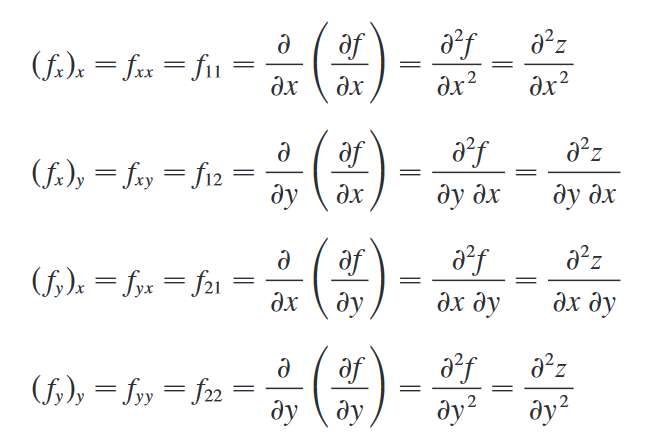
\includegraphics[scale=0.6]{example15-3-1.png}
\end{center}

\subsection*{Clairaut's Theorem}
Suppose $f$ is defined on a disk $D$ that contains the point $(a, b)$.
If the functions $f_{xy}$ and $f_{yx}$ are both continuous on D, then
$f_{xy}(a, b)$ = $f_{yx}(a, b)$

\subsection*{Example}
Calculate $f_{xxyz}$ if $f(x, y, z) = sin(3x + yz)$
\begin{enumerate}
    \item[] $f_x = 3cos(3x + yz)$
    \item[] $f_{xx} = -9sin(3x + yz)$
    \item[] $f_{xxy} = -9zcos(3x + yz)$
    \item[] $f_{xxyz} = -9cos(3x + yz) + 9yzsin(3x + yz)$
\end{enumerate}

\section{Tangent Planes and Linear Approx}
Suppose $f$ has continuous partial derivatives. An equation of the tangent plane
to the surface $z = f(x, y)$ at the point $P(x_o, y_o, z_o)$ is
$$z-z_0=f_x(x_0,y_0)(x-x_0)+f_y(x_0,y_0)(y-y_0)$$

\subsection*{Example}
Find the tangent plane to the elliptic paraboloid $z=2x2+y2$ at the point $(1, 1, 3)$.

\subsection*{Solution}
Let $f(x, y) =  2x^2 + y^2$. Then
$$f_x(x, y) = 4x \qquad f_y(x, y) = 2y$$
$$f_x(1, 1) = 4 \qquad f_y(1, 1) = 2$$
The equation of the tangent plane at $(1, 1, 3)$ is
$$z - 3 = 4(x - 1) + 2(y - 1)$$
$$\text{or} \qquad z = 4x + 2y - 3$$
Figure (a) shows the elliptic paraboloid and its tangent plane at $(1,1,3)$. Figures
(b) and (c) are zoomed in towards the point $(1,1,3)$. The more we zoom, the flatter the graph appears.
\begin{center}
    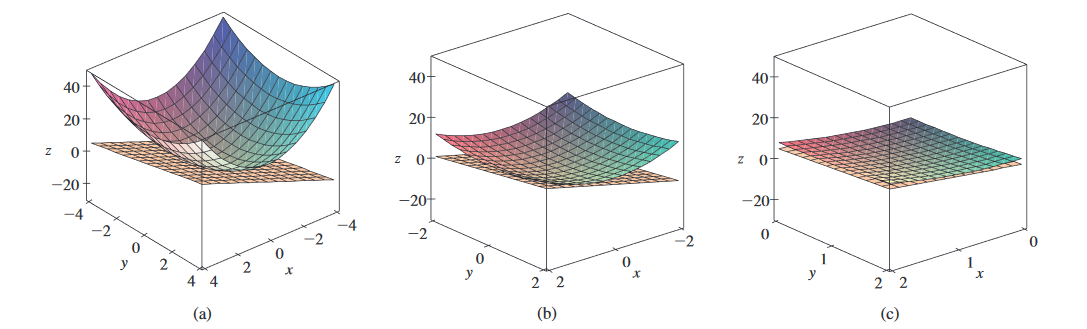
\includegraphics[scale=0.5]{example15-4-1.png}
\end{center}

\subsection*{Definition}
If $z=f(x,y)$, then $f$ is differentiable at $(a,b)$ if $\Delta z$ can be expressed
in the form
$$\Delta z=f_x(a,b)\Delta x+f_y(a,b)\Delta y+\epsilon_1\Delta x+\epsilon_2\Delta y$$
Where $\epsilon_1$ and $\epsilon_2 \to 0$ as $(\Delta x, \Delta y)\to(0,0)$

\subsection*{Theorem}
If the partial derivatives $f_x$ and $f_y$ exist near $(a, b)$ and are continuous at
$(a, b)$ then $f$ is differentiable at $(a, b)$.

\subsection*{Differentials}
For a differentiable function of two variables $z = f(x, y)$, we define the
\textbf{differentials} $dx$ and $dy$ to be independent variables; that is, they can be
given any values. Then the \textbf{differential} $dz$, also called
the \textbf{total differential}, is defined by
$$dz = f_x(x, y) dx + f_y(x, y) dy = \pdv{z}{x}dx + \pdv{z}{y}dy$$

\subsection*{Example}
\begin{enumerate}[(a)]
    \item If $z=f(x,y)=x^2+3xy-y^2$, find the differential $dz$.
    \item If $x$ changes from 2 to 2.05 and $y$ changes from 3 to 2.96, compare the values of $\Delta z$ and $dz$.
\end{enumerate}

\subsection*{Solution}
\begin{enumerate}[(a)]
    \item $$dz=\pdv{z}{x}dx+\pdv{z}{y}dy=(2x+3y)dx+(3x-2y)dy$$
    \item Putting $x=2$, $dx=\Delta x=0.05$, $y=3$, and $dy=\Delta y=-0.04$, we get
          $$dz=[2(2)+3(3)](0.05)+[3(2)-2(3)](-0.04)=0.65$$
\end{enumerate}
The increment of $z$ is
$$\Delta z=f(2.05,2.96)-f(2,3)$$
$$=[(2.05)^2+3(2.05)(2.96)-(2.96)^2]-[2^2+3(2)(3)-3^2]=6.449$$

\section{The Chain Rule}

\subsection*{The Chain Rule (Case 1)}
Suppose that $z = f(x, y)$ is a differentiable function of $x$ and $y$, where
$x = g(t)$ and $y = h(t)$ are both differentiable functions of $t$. Then
$z$ is a differentiable function of $t$ and
$$\dv{z}{t}=\pdv{f}{x}\dv{x}{t}+\pdv{f}{y}\dv{y}{t}$$

Since we often write $\pdv{z}{x}$ in place of $\pdv{f}{x}$, we can rewrite the Chain
Rule in the form
$$\dv{z}{t}=\pdv{z}{x}\dv{x}{t}+\pdv{z}{y}\dv{y}{t}$$

\subsection*{Example}
The pressure $P$ (in kilopascals), volume $V$ (in liters), and temperature $T$
(in kelvins) of a mole of an ideal gas are related by the equation $PV=8.31T$. Find
the rate at which pressure is chaning when the temperature is 300 K and increasing at
a rate of 0.1 K/s and the volume is 100 L and increasing at a rate of 0.2 L/s.

\subsection*{Solution}
If $t$ represents the time elapsed in seconds, then at the given instant we have
$T=300$, $\dv{T}{t}=0.1$, $V=100$, and $\dv{V}{t}=0.2$. Since
$$P=8.31\frac{T}{V}$$
the Chain Rule gives
$$\dv{P}{t}=\pdv{P}{T}\dv{T}{t}+\pdv{P}{V}\dv{V}{t}=\frac{8.31}{V}\dv{T}{t}-
    \frac{8.31T}{V^2}\dv{V}{t}$$
$$=\frac{8.31}{100}(0.1)-\frac{8.31(300)}{100^2}(0.2)=-0.04155$$
The pressure is decreasing at a rate of about 0.042 kPa/s.

We now consider the situation where $z=f(x,y)$ but each of $x$ and $y$ is a function
of two variables $s$ and $t$: $x=g(s,t)$, $y=h(s,t)$. Then $z$ is indirectly a function
of $s$ and $t$ and we wish to find $\pdv{z}{s}$ and $\pdv{z}{t}$. Recall that in
computing $\pdv{z}{t}$ we hold $s$ fixed and compute the ordinary derivative of $z$
with respect to $t$. Therefore,
$$\pdv{z}{t}=\pdv{z}{x}\pdv{x}{t}+\pdv{z}{y}\pdv{y}{t}$$

\subsection*{The Chain Rule (Case 2)}
Suppose that $z = f(x, y)$ is a differentiable function of $x$ and $y$, where
$x = g(s, t)$ and $y = h(s, t)$ are differentiable functions of $s$ and $t$. Then
$$\pdv{z}{s}=\pdv{z}{x}\pdv{x}{s}+\pdv{z}{y}\pdv{y}{s} \qquad
    \pdv{z}{t}=\pdv{z}{x}\pdv{x}{t}+\pdv{z}{y}\pdv{y}{t}$$

\subsection*{The Chain Rule (General Version)}
Suppose that $u$ is a differentiable function of the $n$ variables
$x_1, x_2, \dots x_n$ and each $x_j$ is a differentiable function of the $m$ variables
$t_1,t_2, \dots , t_m$ . Then $u$ is a function of $t_1,t_2, \dots , t_m$ and
$$\pdv{u}{t_i}=\pdv{u}{x_1}\pdv{x_1}{t_i}+\pdv{u}{x_2}\pdv{x_2}{t_i}+\dots+
    \pdv{u}{x_n}\pdv{x_n}{t_i}$$
for each $i=1,2,\dots ,m$.

\subsection*{Example}
If $u=x^4y+y^2z^3$, where $x=rse^t$, $y=rs^2e^{-t}$, and $z=r^2s\sin{t}$, find the
value of $\pdv{u}{s}$ when $r=2$, $s=1$, $t=0$.

\subsection*{Solution}
We have
$$\pdv{u}{s}=\pdv{u}{x}\pdv{x}{s}+\pdv{u}{y}\pdv{y}{s}+\pdv{u}{z}\pdv{z}{s}$$
$$=(4x^3y)(re^t)+(x^4+2yz^3)(2rse^{-t})+(3y^2z^2)(r^2\sin{t})$$
When $r=2$, $s=1$, and $t=0$, we have $x=2$, $y=2$, and $z=0$, so
$$\pdv{u}{s}=(64)(2)+(16)(4)+(0)(0)=192$$

\subsection*{Example}
If $g(s,t)=f(s^2-t^2,t^2-s^2)$ and $f$ is differentiable, show that $g$ satisfies
the equation
$$t\pdv{g}{s}+s\pdv{g}{t}=0$$

\subsection*{Solution}
Let $x=s^2-t^2$ and $y=t^2-s^2$. Then $g(s,t)=f(x,y)$ and the Chain Rule gives
$$\pdv{g}{s}=\pdv{f}{x}\pdv{x}{s}+\pdv{f}{y}\pdv{y}{s}=\pdv{f}{x}(2s)+\pdv{f}{y}(-2s)$$
$$\pdv{g}{t}=\pdv{f}{x}\pdv{x}{t}+\pdv{f}{y}\pdv{y}{t}=\pdv{f}{x}(-2t)+\pdv{f}{y}(2t)$$
Therefore
$$t\pdv{g}{s}+s\pdv{g}{t}=\left(2st\pdv{f}{x}-2st\pdv{f}{y}\right)+
    \left(-2st\pdv{f}{x}+2st\pdv{f}{y}\right)=0$$

\subsection*{Implicit Differentiation}
$$\dv{y}{x}=-\frac{\pdv{F}{x}}{\pdv{F}{y}}=-\frac{F_x}{F_y}$$
To derive this equation we assumed that $F(x, y) = 0$ defines $y$ implicitly as a
function of $x$. The \textbf{Implicit Function Theorem}, proved in advanced calculus,
gives conditions under which this assumption is valid. It states that if $F$ is
defined on a disk containing $(a, b)$, where $F(a, b) = 0$, $F_y(a, b)\neq 0$,
and $F_x$ and $F_y$ are continuous on the disk, then the equation $F(x, y) = 0$
defines $y$ as a function of $x$ near the point $(a, b)$ and the derivative of
this function is given by that equation.

\section{Directional Derivatives and the Gradient Vector}

\subsection*{Directional Derivatives}

\subsection*{Definition}
The \textbf{directional derivative} of $f$ at $(x_0,y_0)$ in the direction of
a unit vector $\textbf{u}=\ev{a,b}$ is
$$D_uf(x_0,y_0)=\lim_{h\to 0}\frac{f(x_0+ha,y_0+hb)-f(x_0,y_0)}{h}$$
if this limit exists.

\subsection*{Example}
Use the weather map in the figure to estimate the value of the directional derivative
of the temperature function at Reno in the southeasterly direction.

\subsection*{Solution}
The unit vector directed toward the southeast is $\mathbf{u=(i-j)}/\sqrt{2}$, but we
won't need to use this expression. We start by drawing a line through Reno toward
the southeast.
\begin{center}
    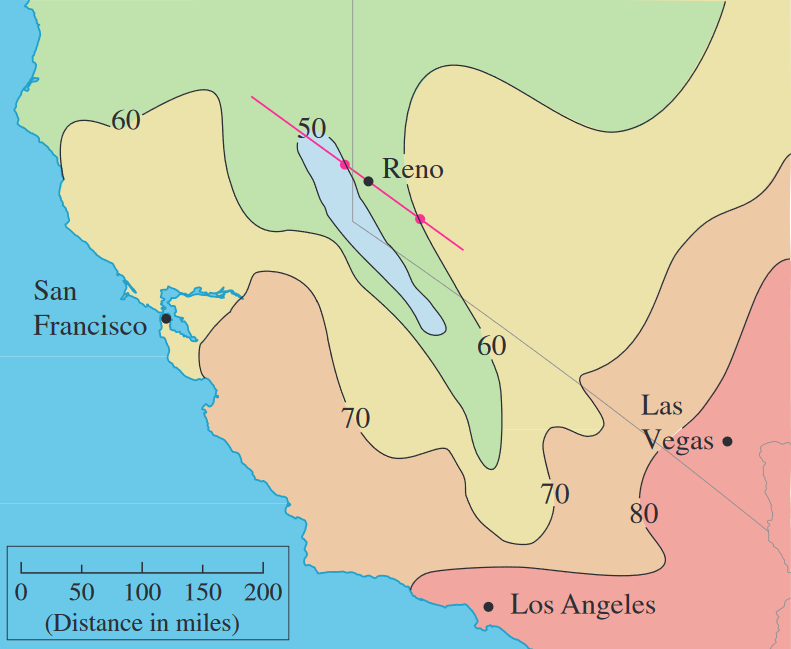
\includegraphics[scale=0.5]{example15-6-1.png}
\end{center}
We approximate the directional derivative $D_uT$ by the average rate of change of
the temperature between the points where this line intersects the isothermals
$T=50$ and $T=60$. The temperature at the point southeast of Reno is $T=60^\circ F$ and
the tempera-ture at the point northwest of Reno is $T=50^\circ F$. The distance between
these points looks to be about 75 miles. So the rate of change of the temperature
in the southeasterly direction is
$$D_uT\approx\frac{60-50}{75}=\frac{10}{75}\approx 0.13^\circ F/mi$$

\subsection*{Theorem}
If $f$ is a differentiable function of $x$ and $y$, then $f$ has a directional
derivative in the direction of any unit vector $\textbf{u}=\ev{a,b}$ and
$$D_uT=f_x(x,y)a+f_y(x,y)b$$

\subsection*{Proof}
If we define a function $g$ of the single variable $h$ by
$$g(h)=f(x_0+ha,y_0+hb)$$
then by the definition of a derivative we have
$$g'(0)=\lim_{h\to 0}\frac{g(h)-g(0)}{h}=\lim_{h\to 0}\frac{f(x_0+ha,y_0+hb)-f(x_0,y_0)}{h}$$
$$=D_uf(x_0,y_0)$$
On the other hand, we can write $g(h)=f(x,y)$, where $x=x_0+ha$, $y=y_0+hb$, so the
Chain Rule gives
$$g'(h)=\pdv{f}{x}\dv{x}{h}+\pdv{f}{y}\dv{y}{h}=f_x(x,y)a+f_y(x,y)b$$
If we now put $h=0$, then $x=x_0$, $y=y_0$, and
$$g'(0)=f_x(x_0,y_0)a+f_y(x_0,y_0)b$$
Comparing the two equations for $g'(0)$, we see that
$$D_uf(x_0,y_0)=f_x(x_0,y_0)a+f_y(x_0,y_0)b$$
If the unit vector \textbf{u} makes an angle $\theta$ with the positive $x$-axis, then
we can write $\textbf{u}=\ev{\cos{\theta},\sin{\theta}}$ and the formula in the previous theorem becomes
$$D_uf(x,y)=f_x(x,y)\cos{\theta}+f_y(x,y)\sin{\theta}$$

\subsection*{Definition}
If $f$ is a function of two variables $x$ and $y$, then the gradient of $f$ is
the vector function $\nabla f$ defined by
$$\nabla f(x,y)=\ev{f_x(x,y),f_y(x,y)}=\pdv{f}{x}\ihat\pdv{f}{y}\jhat$$

\subsection*{Definition}
The directional derivative of $f$ at $\ev{x_0, y_0, z_0}$ in the direction
of a unit vector $u = \ev{a, b, c}$ is
$$D_uf(x_0, y_0, z_0)=\lim_{h\to 0}\frac{f(x_0+ha,y_0+hb,z_0+hc)-f(x_0,y_0,z_0)}{h}$$
The compact form is
$$D_uf(x_0)=\lim_{h\to 0}\frac{f(x_0+hu)-f(x_0)}{h}$$

\subsection*{The Gradient Vector}

\subsection*{Definition}
If $f$ is a function of two variables $x$ and $y$, then the \textbf{gradient} of $f$
is the vector function $\nabla f$ defined by
$$\nabla f(x,y)=\ev{f_x(x,y),f_y(x,y)}=\pdv{f}{x}\ihat+\pdv{f}{y}\jhat$$
For a function $f$ of three variables, the \textbf{gradient vector} is
$$\nabla f=\ev{f_x,f_y,f_z}=\pdv{f}{x}\ihat+\pdv{f}{y}\jhat+\pdv{f}{z}\khat$$

\subsection*{Example}
If $f(x,y,z)=x\sin{yz}$, (a) find the gradient of $f$ and (b) find the directional
derivative of $f$ at $(1,3,0)$ in the direction of $\textbf{v}=\ihat+2\jhat-\khat$.

\subsection*{Solution}
\begin{enumerate}[(a)]
    \item The gradient of $f$ is
          $$\nabla f(x,y,z)=\ev{f_x(x,y,z),f_y(x,y,z),f_z(x,y,z)}$$
          $$=\ev{\sin{yz},cz\cos{yz},xy\cos{yz}}$$
    \item At $(1,3,0)$ we have $\nabla f(1,3,0)=\ev{0,0,3}$. The unit vector in the
          direction of $\textbf{v}=\ihat+2\jhat-\khat$ is
          $$\textbf{u}=\frac{1}{\sqrt{6}}\ihat+\frac{2}{\sqrt{6}}\jhat-\frac{1}{\sqrt{6}}\khat$$
          Therefore, $D_uf(x,y,z)=\nabla f(x,y,z) \cdot \textbf{u}$ gives us
          $$D_uf(1,3,0)=\nabla f(1,3,0)\cdot\textbf{u}$$
          $$=3\khat\cdot\left(\frac{1}{\sqrt{6}}\ihat+\frac{2}{\sqrt{6}}\jhat-\frac{1}{\sqrt{6}}\khat\right)$$
          $$=3\left(-\frac{1}{\sqrt{6}}\right)=-\sqrt{\frac{3}{2}}$$
\end{enumerate}

\subsection*{Theorem}
Suppose $f$ is a differentiable function of two or three variables. The maximum
value of the directional derivative $D_uf(x)$ is $|\nabla f(x)|$ and it occurs
when \textbf{u} has the same direction as the gradient vector $\nabla f(x)$

\subsection*{Proof}
We have
$$D_uf=\nabla f\cdot\textbf{u}=|\nabla f||\textbf{u}|\cos{\theta}=|\nabla f|\cos{\theta}$$
Where $\theta$ is the angle between $\nabla f$ and \textbf{u}. The maximum value of $\cos{\theta}$ is 1
and this occurs when $\theta = 0$. Therefore, the maximum value of $D_uf$ is $|\nabla f|$ and
it occurs when $\theta = 0$, that is, when \textbf{u} has the same direction as $\nabla f$

\section{Maximum and Minimum Values}

\subsection*{Definition}
A function of two variables has a {local maximum} at $(a, b)$ if $f(x, y)\leq f(a, b)$
when $(x, y)$ is near $(a, b)$. The number $f(a, b)$ is called a \textbf{local maximum value},
if $f(x, y)\geq f(a, b)$ when $(x, y)$ is near $(a, b)$, then $f(a, b)$ is a \textbf{local minimum value}.

\subsection*{Theorem}
If $f$ has a local maximum or minimum at $(a, b)$ and the first-order partial
derivatives of $f$ exist there, then $f_x (a, b) = 0$ and $f_y (a, b) = 0$.

\subsection*{Example}
Let $f(x,y)=x^2+y^2-2x-6y+14$. Then
$$f_(x,y)=2x-2 \qquad f_y(x,y)=2y-6$$
These partial derivatives are equal to 0 when $x=1$ and $y=3$, so the only critical
point is $(1,3)$. By completing the square, we find that
$$f(x,y)=4+(x-1)^2+(y-3)^2$$
Since $(x-1)^2\geq 0$ and $(y-3)^2\geq 0$, we have $f(x,y)\geq 4$ for all values of
$x$ and $y$. Therefore $f(1,3)=4$ is a local minimum, and in fact it is the absolute
minimum of $f$. This can be confirmed geometrically from the graph of $f$, which is the
elliptic paraboloid with vertex $(1,3,4)$.

\subsection*{Second Derivatives Test}
Suppose the second partial derivatives of $f$ are continuous on a disk with center
$(a, b)$, and suppose that $f_x (a, b) = 0$ and $f_y (a, b) = 0$ Let
$$D=D(a,b)=f_{xx}(a,b)f_{yy}(a,b)-[f_{xy}(a,b)]^2$$
\begin{enumerate}[(a)]
    \item If $D > 0$ and $f_{xx}(a, b) > 0$, then $f(a, b)$ is a local minimum
    \item If $D > 0$ and $f_{xx}(a, b) < 0$, then $f(a, b)$ is a local maximum
    \item If $D < 0$, then $f(a, b)$ is not a local maximum or minimum
\end{enumerate}

\subsection*{Example}
Find the local maximum and minimum values and saddle points of $f(x,y)=x^4+y^4-4xy+1$.

\subsection*{Solution}
We first locate the critical points:
$$f_x=4x^3-4y \qquad f_y=4y^3-4x$$
Setting these partial derivatives equal to 0, we obtain the equations
$$x^3-y=0 \qquad \text{and} \qquad y^3-x=0$$
To solve these equations we substitute $y=x^3$ from the first equation into the
second one. This gives
$$0=x^9-x=x(x^8-1)=x(x^4-1)(x^4+1)=x(x^2-1)(x^2+1)(x^4+1)$$
so there are three real roots: $x=0$, 1, -1. The three critical points are $(0,0)$,
$(1,1)$, and $(-1,-1)$. Next we calculate the second partial derivatives and $D(x,y)$:
$$f_{xx}=12x^2 \qquad f_{xy}=-4 \qquad f_{yy}=12y^2$$
$$D(x,y)=f_{xx}f_{yy}-(f_{xy})^2=144x^2y^2-16$$
Since $D(0,0)=-16<0$, it follows that form case (c) of the Second Derivatives Test that
the origin is a saddle point; that is, $f$ has no local maximum or minimum at $(0,0)$.
Since $D(1,1)=128>0$ and $f_{xx}(1,1)=12>0$, we see from case (a) of the test that
$f(1,1)=-1$ is a local minimum. Similarlym we have $D(-1,-1)=128>0$ and
$f_{xx}(-1,-1)=12>0$, so $f(-1,-1)=-1$ is also a local minimum. The graph of $f$ is shown below.
\begin{center}
    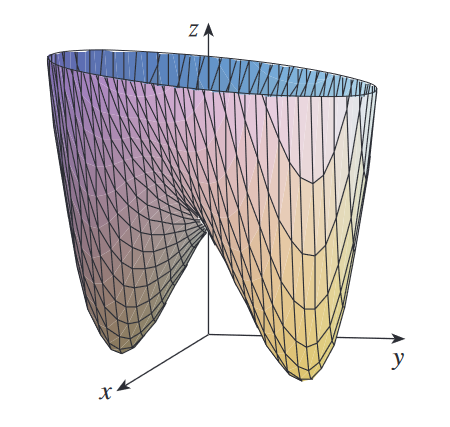
\includegraphics[scale=0.7]{example15-7-1.png}
\end{center}

\subsection*{Extreme Value Theorem for Functions of Two Variables}
If $f$ is continuous on a closed, bounded set $D$ in $\mathbb{R}^2$, then $f$
attains an absolute maximum value $f(x_1, y_1)$ and an absolute minimum value $f(x_2, y_2)$
at some points $(x_1, y_1)$ and $(x_2, y_2)$ in $D$.

To find the absolute maximum and minimum values of a continuous function $f $
on a closed, bounded set $D$:
\begin{enumerate}
    \item Find the values of $f$ at the critical points of $f$ in $D$
    \item Find the extreme values of $f$ on the boundary of $D$
    \item The largest of the values from steps 1 and 2 is the absolute maximum value;
          the smallest of these values is the absolute minimum value.
\end{enumerate}

\section{Lagrange Multipliers}

\subsection*{Method of Lagrange Multipliers}
To find the maximum and minimum values of $f(x, y, z) $subject to the
constraint $g(x, y, z) = k$:
\begin{enumerate}[(a)]
    \item Find all values of $x$, $y$, $z$, and $\lambda$ such that
          $$\nabla f(x,y,z)=\lambda\nabla g(x,y,z) \qquad \text{and} \qquad g(x,y,z)=k$$
    \item Evaluate $f$ at all points $(x, y, z)$ that result from step (a). The largest
          of these values is the maximum value of $f$; the smallest is the minimum value of $f$
\end{enumerate}

\subsection*{Example}
A rectangular box without a lid is to be made from $12\text{m}^2$ of cardboard.
Find the maximum volume of such a box.

\subsection*{Solution}
We let $x$, $y$, and $z$ be the length, width, and height, respectively, of the box in
meters. Then we wish to maximize
$$V=xyz$$
subject to the constraint
$$g(x,y,z)=2xz+2yz+xy=12$$
Using the method of lagrange multipliers, we look for values of $x$, $y$, $z$,
and $\lambda$ such that $\nabla V= \lambda\nabla g$ and $g(x, y, z) = 12$. This gives the equations
$$V_x=\lambda g_x \qquad V_y=\lambda g_y \qquad V_z=\lambda g_z \qquad 2xz+2yz+xy=12$$
which become
\begin{enumerate}
    \item[(2)] $yz=\lambda(2z+y)$
    \item[(3)] $xz=\lambda(2z+x)$
    \item[(4)] $xy=\lambda(2x+2y)$
    \item[(5)] $2xz+2yz+xy=12$
\end{enumerate}
There are no general rules for solving systems of equations. Sometimes ingenuity
is required. In the present example you might notice that if we multiply (2)
by $x$, (3) by $y$, and (4) by $z$, then the left sides of these equations will be
identical. We get
\begin{enumerate}
    \item[(6)] $xyz=\lambda(2xz+xy)$
    \item[(7)] $xyz=\lambda(2yz+xy)$
    \item[(8)] $xyz=\lambda(2xz+2yz)$
\end{enumerate}
We observe that $\lambda$ is  not equal to 0 because $\lambda = 0$ would imply
$yz - xz - xy = 0$. From (2), (3), and (4) and this would contradict (5).
Therefore, from (6) and (7) we have
$$2xz+xy=2yz+xy$$
which gives $xz=yz$. But $z\neq 0$ (since $z=0$ would give $V=0$), so $x=y$.
From (7) and (8) we have
$$2yz+xy=2xz+2yz$$
which gives $2xz=xy$ and so (since $x\neq 0$) $y=2z$. If we now put $x=y=2z$ in (5), we get
$$4z^2+4z^2+4z^2=12$$
Since $x$, $y$, and $z$ are all positive, we therefore have $z=1$ and so $x=2$ and $y=2$.

\subsection*{Example}
Find the maximum value of the function $f(x,y,z)=x+2y+3z$ on the curve of the
intersection of the plane $x-y+z=1$ and the cylinder $x^2+y^2=1$.

\subsection*{Solution}
We maximum the function $f(x,y,z)=x+2y+3z$ subject to the constraints $g(x,y,z)=x-y+z=1$
and $h(x,y,z)=x^2+y^2=1$. The Lagrange condition is $\nabla f=\lambda\nabla g+\mu\nabla h$,
so we solve the equations
\begin{enumerate}
    \item[(17)] $1=\lambda+2x\mu$
    \item[(18)] $2=-\lambda+2y\mu$
    \item[(19)] $3=\lambda$
    \item[(20)] $x-y+z=1$
    \item[(21)] $x^2+y^2=1$
\end{enumerate}
Putting $\lambda=3$ /[from (19)/] in (17), we get $2x\mu=-2$, so $x=-1/\mu$. Similarly,
(18) gives $y=5/(2\mu)$. Substitution in (21) then gives
$$\frac{1}{\mu^2}+\frac{25}{4\mu^2}=1$$
and so $\mu^2=\frac{29}{4}$, $\mu=\pm\sqrt{29}/2$. Then $x=\mp 2/sqrt{29}$,
$y=\pm 5/\sqrt{29}$, and, from (2), $z=1-x+y=1\pm 7/\sqrt{29}$. The corresponding values of $f$ are
$$\mp\frac{2}{\sqrt{29}}+2\left(\pm\frac{5}{\sqrt{29}}\right)+3\left(1\pm\frac{7}{\sqrt{29}}\right)=
    3\pm\sqrt{29}$$
Therefore, the maximum value of $f$ on the given curve is $3+\sqrt{29}$.
\chapter{Multiple Integrals}

\section{Double Integrals over Rectangles}

\subsection*{Definition}
Definition The \textbf{double integral} of $f$ over the rectangle $R$ is
$$\iint\limits_R f(x,y)\:dA=\lim_{m,n\to\infty}\sum_{i=1}^m\sum_{j=1}^n f(x_{ij}^*,y_{ij}^*) \Delta A$$
if this limit exists.

If $f(x, y) \geq 0,$ then the volume V of the solid that lies above the rectangle $R$ and
below the surface $z = f(x, y)$ is
$$V=\iint\limits_R f(x,y)\:dA$$

\subsection*{Example}
Estimate the volume of the solid that lies above the square $R=[0,2]\times[0,2]$
and below the elliptic paraboloid $z=16-x^2-2y^2$. Divide R into four equal squares
and choose the sample point to be the upper right corner of each square $R_{ij}$.
Sketch the solid and the approximating rectangular boxes.

\subsection*{Solution}
The squares are shown below. The paraboloid is the graph of
$f(x,y)=16-x^2-2y^2$ and the area of each square is $\Delta A=1$. Approximating
the volume by the Riemann sum with $m=n=2$, we have
\begin{align*}
    V & \approx\sum_{i=1}^2\sum_{j=1}^2 f(x_i,y_j) \delta A          \\
      & =f(1,1)\delta A+f(1,2)\delta A+f(2,1)\delta A+f(2,2)\delta A \\
      & =13(1)+7(1)+10(1)+4(1)=34
\end{align*}
\begin{center}
    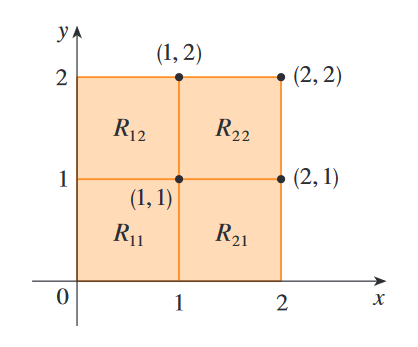
\includegraphics[scale=0.6]{example16-1-1.png}
\end{center}

We get better apprximations to the volume if we increase the number of squares.
Shown below is how the columns look more like the actual solid when we use 16, 64, and 256 squares.
\begin{center}
    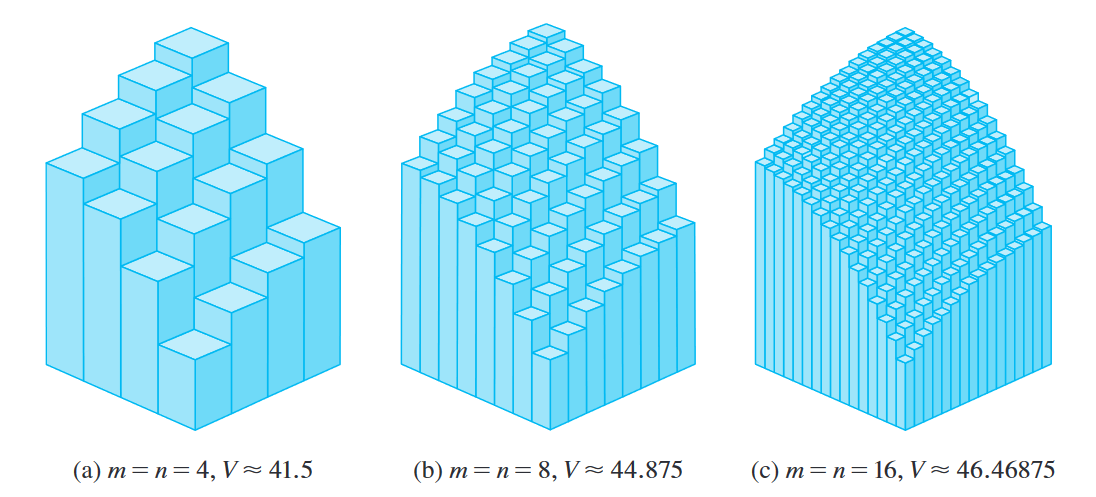
\includegraphics[scale=0.5]{example16-1-2.png}
\end{center}

\subsection*{Midpoint Rules for Double Integrals}
$$\iint\limits_R f(x,y)\:dA\approx\sum_{i=1}^m\sum_{j=1}^n f(\bar{x}_i,\bar{y}_j)\Delta A$$
where $\bar{x}_i$ is the midpoint of $[x_{i-1},x_i]$ and $\bar{y}_j$ is the midpoint
of $[y_{j-1},y_j]$.

\subsection*{Example}
Use the Midpoint Rule with $m=n=2$ to estimate the value of the integral
$\iint\limits_R (x-3y^2)\:dA$, where $R=\{(x,y)\:|\:0\leq x\leq 2, 1\leq y\leq 2\}$.

\subsection*{Solution}
In using the Midpoint Rule with $m=n=2$, we evaluate $f(x,y)=x-3y^2$ at the centers
of the four subrectangles shown below. So $\bar{x}_1=\frac{1}{2}$, $\bar{x}_2=\frac{3}{2}$,
$\bar{y}_1=\frac{5}{4}$, and $\bar{y}_2=\frac{7}{4}$. The area of each subrectangle
is $\Delta A=\frac{1}{2}$. Thus
\begin{align*}
    \iint\limits_R (x-3y^2)\:dA & \approx\sum_{i=1}^2\sum_{j=1}^2 f(\bar{x}_i,\bar{y}_j)\Delta A                                                                                                                           \\
                                & =f(\bar{x}_1,\bar{y}_1)\Delta A+f(\bar{x}_1,\bar{y}_2)\Delta A+f(\bar{x}_2,\bar{y}_1)\Delta A+f(\bar{x}_2,\bar{y}_2)\Delta A                                                             \\
                                & =f\left(\frac{1}{2},\frac{5}{4}\right)\Delta A+f\left(\frac{1}{2},\frac{7}{4}\right)\Delta A+f\left(\frac{3}{2},\frac{5}{4}\right)\Delta A+f\left(\frac{3}{2},\frac{7}{4}\right)\Delta A \\
                                & =\left(-\frac{67}{16}\right)\frac{1}{2}+\left(-\frac{139}{16}\right)\frac{1}{2}+\left(-\frac{51}{16}\right)\frac{1}{2}+\left(-\frac{123}{16}\right)\frac{1}{2}                           \\
                                & =-\frac{95}{8}=-11.875
\end{align*}
Thus we have
$$\iint\limits_R (x-3y^2)\:dA\approx -11.875$$

\subsection*{Average Value}
The average value of a function $f$ of one variable is
$$f_{ave}=\frac{1}{b-a}\int_a^b f(x)\:dx$$
Similarly, the \textbf{average value} of a function $f$ of two variables defined on
a rectangle $R$ is
$$f_{ave}=\frac{1}{A(R)}\iint\limits_R f(x,y)\:dA$$
where $A(R)$ is the area of $R$.

\section{Iterated Integrals}

\subsection*{Example}
Evaluate the iterated integrals.
\begin{enumerate}[(a)]
    \item $\int_0^3 \int_1^2 x^2y\:dy\:dx$
    \item $\int_1^2 \int_0^3 x^2y\:dx\:dy$
\end{enumerate}

\subsection*{Solution}
\begin{enumerate}[(a)]
    \item Regarding $x$ as a constant, we obtain
          $$\int_1^2 x^2y\:dy=\left[x^2\frac{y^2}{2}\right]_{y=1}^{y=2}$$
          $$=x^2\left(\frac{2^2}{2}\right)-x^2\left(\frac{1^2}{2}\right)=\frac{3}{2}x^2$$
          Thus, the function $A$ in the preceding discussion is given by $A(x)=\frac{3}{2}x^2$
          in this example. We now integrate this function of $x$ from 0 to 3:
          $$\int_0^3 \int_1^2 x^2y\:dy\:dx=\int_0^3\left[\int_1^2 x^2y\:dy\right]\:dx$$
          $$=\int_0^3 \frac{3}{2}x^2\:dx=\left[\frac{x^3}{2}\right]_0^3=\frac{27}{2}$$
    \item Here we first integrate with respect to $x$:
          $$\int_1^2 \int_0^3 x^2y\:dx\:dy=\int_1^2\left[\int_0^3 x^2y\:dx\right]\:dy=
              \int_1^2\left[\frac{x^3}{3}y\right]_{x=0}^{x=3}\:dy$$
          $$=\int_1^2 9y\:dy=\left[9\frac{y^2}{2}\right]_1^2=\frac{27}{2}$$
          Notice that we obtained the same answer whether we integrated with respect to
          $y$ or $x$ first. The order of integration doesn't matter.
\end{enumerate}

\subsection*{Fubini's Theorem}
If $f$ is continuous on the rectangle $R=\{(x,y)\:|\:a\leq x\leq b,\: c\leq y\leq d\}$ then
$$\iint\limits_R f(x,y)\: dA=\int_a^b\int_c^d f(x,y)\:dy\:dx=\int_c^d\int_a^b f(x,y)\:dx\:dy$$
More generally, this is true if we assume that $f$ is bounded on $R$, $f$ is discontinuous
only on a finite number of smooth curves, and the iterated integrals exist.

\subsection*{Example}
If $R=[0,\pi/2]\times[0,\pi/2]$, then
$$\iint\limits_R \sin{x}\cos{y}\:dA=\int_0^{\pi/2}\sin{x}\:dx\int_0^{\pi/2}\cos{y}\:dy$$
$$=[-\cos{x}]_0^{\pi/2}[\sin{y}]_0^{\pi/2}=1\cdot 1=1$$
\begin{center}
    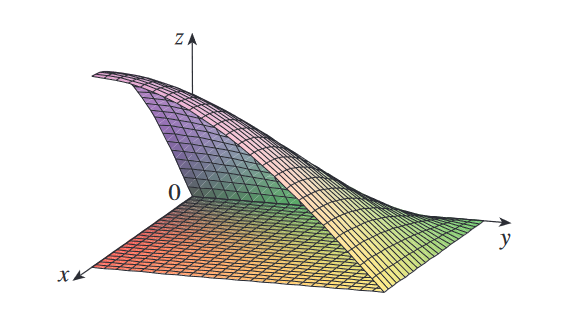
\includegraphics[scale=0.6]{example16-2-1.png}
\end{center}

\section{Double Integrals over General Regions}

If $F$ is integrable over $R$, then we define the \textbf{double integral of $f$ over $D$} by
$$\iint\limits_D f(x,y)\:dA=\iint\limits_R F(x,y)\:dA$$

If $f$ is continuous on a type I region $D$ such that
$$D=\left\{(x,y)\:|\: a\leq x\leq b,|\: g_1(x)\leq y\leq g_2(x)\right\}$$
then
$$\iint\limits_D f(x,y)\:dA=\int_a^b\int_{g_1(x)}^{g_2(x)}f(x,y)\:dy\:dx$$

Using the same methods as above, we can show that
$$\iint\limits_D f(x,y)\:dA=\int_c^d\int_{h_1(y)}^{h_2(y)}f(x,y)\:dx\:dy$$
where $D$ is a type II region.

\subsection*{Example}
Evaluate $\int\limits_D (x+2y)\:dA$, where $D$ is the region bounded by the parabolas
$y=2x^2$ and $y=1+x^2$

\subsection*{Solution}
The parabolas intersect when $2x^2=1+x^2$, that is, $x^2=1$, so $x=\pm 1$. We note
that the region $D$, is a type I region but not a type II region and we can write
$$D=\{(x,y)\:|\: -1\leq x\leq 1,\: 2x^2\leq y\leq 1+x^2\}$$
Since the lower boundary is $y=2x^2$ and the upper boundary is $y=1+x^2$, we have
\begin{align*}
    \iint\limits_D(x+2y)\:dA & =\int_{-1}^1\int_{2x^2}^{1+x^2} (x+2y)\:dy\:dx                                                  \\
                             & =\int_{-1}^1\left[xy+y^2\right]_{y=2x^2}^{y=1+x^2}\:dx                                          \\
                             & =\int_{-1}^1\left[x(1+x^2)+(1+x^2)^2-x(2x^2)-(2x^2)^2\right]\:dx                                \\
                             & =\int_{-1}^1(-3x^4-x^3+2x^2+x+1)\:dx                                                            \\
                             & =\left[-3\frac{x^5}{5}-\frac{x^4}{4}+2\frac{x^3}{3}+\frac{x^2}{2}+x\right]_{-1}^1=\frac{32}{15}
\end{align*}

\subsection*{Example}
Evaluate $\iint\limits_D xy\:dA$, where $D$ is the region bounded by the line $y=x-1$
and the parabola $y^2=2x+6$.

\subsection*{Solution}
The region $D$ is shown below. Again $D$ is both type I and type II, but the description of $D$ as a type I region is
more complicated because the lower boundary consists of two parts. Therefore, we prefer
to express $D$ as a type II region:
$$D=\{(x,y)\:|\:-2\leq y\leq 4,\: \frac{1}{2}y^2-3\leq x\leq y+1\}$$
\begin{center}
    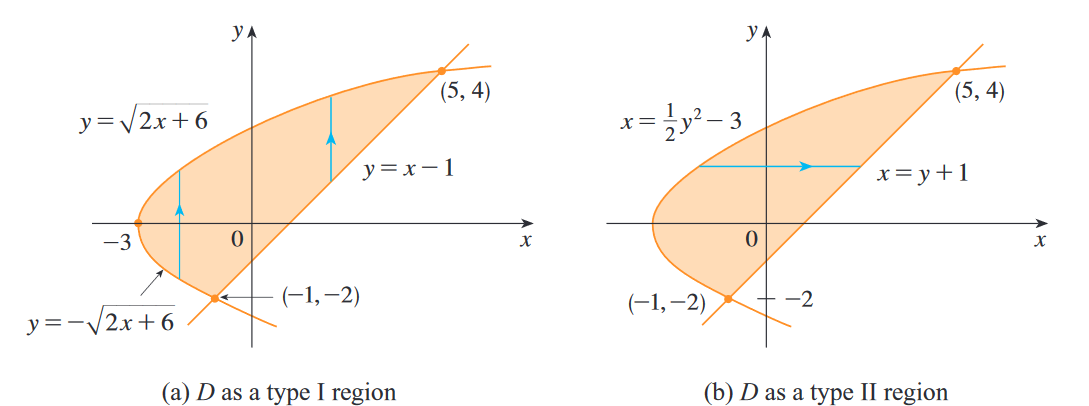
\includegraphics[scale=0.5]{example16-3-1.png}
\end{center}
\begin{align*}
    \iint\limits_D xy\:dA & =\int_{-2}^4\int_{\frac{1}{2}y^2-3}^{y+1}xy\:dx\:dy=\int_{-2}^4\left[\frac{x^2}{2}y\right]_{x=\frac{1}{2}y^2-3}^{x=y+1}\:dy \\
                          & =\frac{1}{2}\int_{-2}^4 y[(y+1)^2-(\frac{1}{2}y^2-3)^2]\:dy                                                                 \\
                          & =\frac{1}{2}\int_{-2}^4 \left(-\frac{y^5}{4}+4y^3+2y^2-8y\right)\:dy                                                        \\
                          & =\frac{1}{2}\left[-\frac{y^6}{24}+y^4+2\frac{y^3}{3}-4y^2\right]_{-2}^4=36
\end{align*}
If we had expressed $D$ as a type I region using (a), then we would have obtained
$$\iint\limits_D xy\: dA=\int_{-3}^{-1}\int_{-\sqrt{2x+6}}^{\sqrt{2x+6}} xy\:dy\:dx+
    \int_{-1}^5\int_{x-1}^{\sqrt{2x+6}} xy\:dy\:dx$$
but this would have involved more work than the other method.

\subsection*{Properties of Double Integrals}
\begin{enumerate}
    \item[(6)] $\iint\limits_D [f(x,y)+g(x,y)]\:dA=\iint\limits_D f(x,y)\:dA+\iint\limits_D g(x,y)\:dA$
    \item[(7)] $\iint\limits_D cf(x,y)\:dA=c\iint\limits_D f(x,y)\:dA$
    \item[(9)] $\iint\limits_D f(x,y)\:dA=\iint\limits_{D_1} f(x,y)\:dA+\iint\limits_{D_2} f(x,y)\:dA$
    \item[(10)] $\iint\limits_D 1\:dA=A(D)$
    \item[(11)] If $m\leq f(x,y)\leq M$ for all $(x,y)$ in $D$, then $$mA(D)\leq\iint\limits_D f(x,y)\:dA\leq MA(D)$$
\end{enumerate}

\subsection*{Example}
Use Property 11 to estimate the integral $\iint\limits_D e^{\sin{x}\cos{y}}\:dA$,
where $D$ is the disk with center the origin and radius 2.

\subsection*{Solution}
Since $-1\leq\sin{x}\leq 1$ and $-1\leq \cos{y}\leq 1$, we have $-1\leq\sin{x}\cos{y}\leq 1$
and therefore
$$e^{-1}\leq e^{\sin{x}\cos{y}}\leq e^1=e$$
Thus, using $m=e^{-1}=1/e$, $M=e$, and $A(D)=\pi(2)^2$ in Property 11, we obtain
$$\frac{4\pi}{e}\leq\iint\limits_D e^{\sin{x}\cos{y}}\:dA\leq 4\pi e$$

\section{Double Integrals in Polar Coordinates}

\subsection*{Change to Polar Coordinates in a Double Integral}
If $f$ is continuous on a polar rectangle $R$ given by $0\leq a\leq r\leq b$,
$\alpha\leq\theta\leq\beta$, where $0\leq\beta-\alpha\leq 2\pi$, then
$$\iint\limits_R f(x,y)\:dA=\int_\alpha^\beta\int_a^b f(r\cos{\theta},r\sin{\theta})\:r\:dr\:d\theta$$

\subsection*{Example}
Find the volume of the solid bounded by the plane $z=0$ and the paraboloid $z=1-x^2-y^2$.

\subsection*{Solution}
If we put $z=0$ in the equation of the paraboloid, we get $x^2+y^2=1$. This means that
the plane intersects the paraboloid in the circle $x^2+y^2=1$, so the solid lies under
the paraboloid and above the circular disk $D$ given by $x^2+y^2\leq 1$. In polar
coordinates $D$ is given by $0\leq r\leq 1$, $0\leq\theta\leq 2\pi$ Since
$1-x^2-y^2=1-r^2$, the volume is
\begin{align*}
    V & =\iint\limits_D (1-x^2-y^2)\:dA=\int_0^{2\pi}\int_0^1 (1-r^2)\:r\:dr\:d\theta                             \\
      & =\int_0^{2\pi}\:d\theta\int_0^1(r-r^3)\:dr=2\pi\left[\frac{r^2}{2}-\frac{r^4}{4}\right]_0^1=\frac{\pi}{2}
\end{align*}
If we had used rectangular coordinates instead of polar coordinates, then we would have obtained
$$V=\iint\limits_D(1-x^2-y^2)\:dA=\int_{-1}^1\int_{-\sqrt{1-x^2}}^{\sqrt{1-x^2}}
    (1-x^2-y^2)\:dy\:dx$$
which is not easy to evaluate because it involves finding the following integrals:
$$\int\sqrt{1-x^2}\:dx \qquad \int x^2\sqrt{1-x^2}\:dx \qquad \int(1-x^2)^{3/2}\:dx$$

If $f$ is continuous on the polar region of the form
$$D=\left\{(r,\theta)\:|\:\alpha\leq\theta\beta,\: h_1(\theta)\leq r\leq h_2(\theta)\right\}$$
then
$$\iint\limits_D f(x,y)\:dA=\int_\alpha^\beta\int_{h_1(\theta)}^{h_2(\theta)}
    f(r\cos{\theta}, r\sin{\theta})\:r\:dr\:d\theta$$

\subsection*{Example}
Use a double integral to find the area enclosed by one loop of the four-leaved rose
$r=\cos{2\theta}$.
\begin{center}
    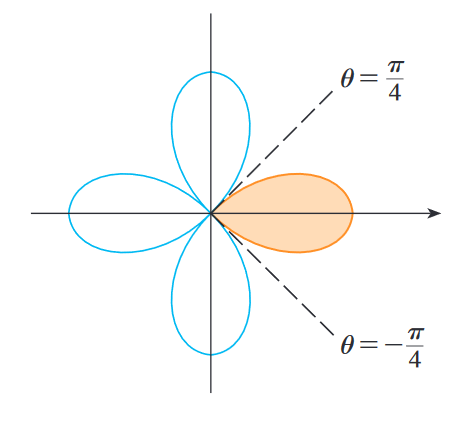
\includegraphics[scale=0.5]{example16-4-1.png}
\end{center}

\subsection*{Solution}
We see that the loop is given by the region
$$D=\{(r,\theta)\:|\:-\pi/4\leq\theta\leq\pi/4.\:0\leq r\leq\cos{2\theta}\}$$
So the area is
\begin{align*}
    A(D) & =\iint\limits_D dA=\int_{-\pi/4}^{\pi/4}\int_0^{\cos{2\theta}}r\:dr\:d\theta                                                                       \\
         & =\int_{-\pi/4}^{\pi/4}\left[\frac{1}{2}r^2\right]_0^{\cos{2\theta}}d\theta=\frac{1}{2}\int_{-\pi/4}^{\pi/4} \cos^2{2\theta}\:d\theta               \\
         & =\frac{1}{4}\int_{-\pi/4}^{\pi/4}(1+\cos{4\theta})\:d\theta=\frac{1}{4}\left[\theta+\frac{1}{4}\sin{4\theta}\right]_{-\pi/4}^{\pi/4}=\frac{\pi}{8}
\end{align*}

\section{Applications of Double Integrals}

\subsection*{Density and Mass}
$$\rho(x,y)=\lim\frac{\Delta m}{\Delta A}$$
$$m=\lim_{k,l\to\infty}\sum_{i=1}^k\sum_{j=1}^l\rho(x_{ij}^*,y_{ij}^*)\Delta A=
    \iint\limits_D\rho(x,y)\:dA$$

\subsection*{Example}
Charge is distributed over the triangular region $D$ in the figure so that the charge
density at $(x,y)$ is $\sigma(x,y)=xy$, measured in coulombs per square meter
$(\text{C/m}^2)$. Find the total charge.

\subsection*{Solution}
\begin{align*}
    Q & =\iint_D \sigma(x,y)\:dA=\int_0^1\int_{1-x}^1 xy\:dy\:dx                                                 \\
      & =\int_0^1\left[x\frac{y^2}{2}\right]_{y=1-x}^{y=1}dx=\int_0^1\frac{x}{2}[1^2-(1-x)^2]\:dx                \\
      & =\frac{1}{2}\int_0^1(2x^2-x^3)\:dx=\frac{1}{2}\left[\frac{2x^3}{3}-\frac{x^4}{4}\right]_0^1=\frac{5}{24}
\end{align*}
Thus the total charge is $\frac{5}{24}$ C.

\subsection*{Moments and Centers of Mass}
The \textbf{moment} of the entire lamina \textbf{about the $x$-axis}:
$$M_x=\lim_{m,n\to\infty}\sum_{i=1}^m\sum_{j=1}^n y_{ij}^*\rho(x_{ij}^*,y_{ij}^*)\Delta A=
    \iint\limits_D y\rho(x,y)\:dA$$
Similarly, the \textbf{moment about the $y$-axis} is:
$$M_y=\lim_{m,n\to\infty}\sum_{i=1}^m\sum_{j=1}^n x_{ij}^*\rho(y_{ij}^*,x_{ij}^*)\Delta A=
    \iint\limits_D x\rho(x,y)\:dA$$
The coordinates $(\bar{x},\bar{y})$ of the center of mass of a lamina occupying the region
$D$ and having density function $\rho(x,y)$ are
$$\bar{x}=\frac{M_y}{m}=\frac{1}{m}\iint\limits_D x\rho(x,y)\:dA \qquad
    \bar{y}=\frac{M_x}{m}=\frac{1}{m}\iint\limits_D y\rho(x,y)\:dA$$
where the mass $m$ is given by
$$m=\iint\limits_D \rho(x,y)\:dA$$

\subsection*{Moment of Inertia}
The \textbf{moment of inertia} of the lamina \textbf{about the $x$-axis}:
$$I_x=\lim_{m,n\to\infty}\sum_{i=1}^m\sum_{j=1}^n(y_{ij}^*)^2\rho(x_{ij}^*,y_{ij}^*)\Delta A=
    \iint\limits_D y^2\rho(x,y)\:dA$$
Similarly, the \textbf{moment of inertia about the $y$-axis} is:
$$I_y=\lim_{m,n\to\infty}\sum_{i=1}^m\sum_{j=1}^n(x_{ij}^*)^2\rho(y_{ij}^*,x_{ij}^*)\Delta A=
    \iint\limits_D x^2\rho(x,y)\:dA$$
It is also of interest to consider the \textbf{moment of inertia about the origin}, also
called the \textbf{polar moment of inertia}:
$$I_0=\lim_{m,n\to\infty}\sum_{i=1}^m\sum_{j=1}^n\left[(x_{ij}^*)^2+(y_{ij}^*)^2\right]
    \rho(x_{ij}^*,y_{ij}^*)\Delta A=\iint\limits_D(x^2+y^2)\rho(x,y)\:dA$$
Note that $I_0=I_x+I_y$.

\subsection*{Example}
Find the moments of inertia $I_x$, $I_y$, and $I_0$ of a homogeneous disk $D$ with density
$\rho(x,y)=\rho$ center the origin, and radius $a$.

\subsection*{Solution}
The boundary of $D$ is the circle $x^2+y^2=a^2$ and in polar coordinates $D$ is
described by $0\leq\theta\leq 2\pi$, $0\leq r\leq a$. Let's compute $I_0$ first:
$$I_0=\iint\limits_D(x^2+y^2)\rho\:dA=\rho\int_0^{2\pi}\int_0^{a}r^2r\:dr\:d\theta$$
$$\rho\int_0^{2\pi}d\theta\int_0^ar^3\:dr=2\pi\rho\left[\frac{r^4}{4}\right]_0^a=\frac{\pi\rho a^4}{2}$$
Instead of computing $I_x$ and $I_y$ directly, we use the facts that $I_x+I_y=I_0$ and
$I_x=I_y$ (from the symmetry of the problem). Thus
$$I_x=I_y=\frac{I_0}{2}=\frac{\pi\rho a^4}{4}$$

\subsection*{Example}
The manager of a movie theater determines that the average time movie-goers
wait in line to buy a ticket for this week’s film is 10 minutes and the average
time they wait to buy popcorn is 5 minutes. Assuming that the waiting times are
independent, find the probability that a moviegoer waits a total of less than 20
minutes before taking his or her seat.

\subsection*{Solution}
Assuming that both the waiting time $X$ for the ticket purchase and the waiting time
$Y$ in the refreshment line are modeled by exponential probability density functions,
we can write the individual density functions as
\[
    f_1(x) =
    \begin{cases}
        0                     & \text{if $x<0$}     \\
        \frac{1}{10}e^{-x/10} & \text{if $x\geq 0$}
    \end{cases} \qquad
    f_2(x) =
    \begin{cases}
        0                   & \text{if $y<0$}     \\
        \frac{1}{5}e^{-y/5} & \text{if $y\geq 0$}
    \end{cases}
\]
Since $X$ and $Y$ are independent, the joint density function is the product:
\[
    f(x,y)=f_1(x)f_2(y)=
    \begin{cases}
        \frac{1}{5}e^{-x/10}e^{-y/5} & \text{if $x\geq 0$, $y\geq 0$} \\
        0                            & \text{otherwise}
    \end{cases}
\]
We are asked for the probability that $X+Y<20$:
$$P(X+Y<20)=P((X,Y)\in D)$$
where $D$ is the triangular region given by the area under $y=-x+20$. Thus
\begin{align*}
    P(X+Y<20) & =\iint\limits_D f(x,y)\:dA=\int_0^{20}\int_0^{20-x}\frac{1}{50}e^{-x/10}e^{-y/5}\:dy\:dx \\
              & =\frac{1}{50}\int_0^{20}\left[e^{-x/10}(-5)e^{-y/5}\right]_{y=0}^{y=20-x}\:dx            \\
              & =\frac{1}{10}\int_0^{20}e^{-x/10}(1-e^{(x-20)/5})\:dx                                    \\
              & =\frac{1}{10}\int_0^{20}(e^{-x/10}-e^{-4}e^{x/10})\:dx                                   \\
              & =1+e^{-4}-2e^{-2}\approx 0.7476
\end{align*}
This means that about 75\% of the moviegoers wait less than 20 minutes before taking
their seats.

\section{Surface Area}
We define the \textbf{surface area} of $S$ to be
\begin{align*}
    A(S) & =\lim_{m,n\to\infty}\sum_{i=1}^m\sum_{j=1}^n \Delta T_{ij}                                       \\
         & =\lim_{m,n\to\infty}\sum_{i=1}^m\sum_{j=1}^n\sqrt{[f_x(x_i,y_j)]^2+[f_y(x_i,y_j)]^2+1}\:\Delta A
\end{align*}

The area of the surface with equation $z=f(x, y), (x, y)\in D$,
where $f_x$ and $f_y$ are continuous, is
$$A(S)=\iint\limits_D\sqrt{[f_x(x_i,y_j)]^2+[f_y(x_i,y_j)]^2+1}\:\Delta A)$$

Rewrite it as follows
$$A(S)=\iint\limits_D\sqrt{1+\left(\pdv{z}{x}\right)^2+\left(\pdv{z}{y}\right)^2}\:dA$$

\subsection*{Example}
Find the surface area of the part of the surface $z=x^2+2y$ that lies above the triangular
region $T$ in the $xy$-plane with the vertices $(0,0)$, $(1,0)$, and $(1,1)$.

\subsection*{Solution}
The region $T$ is described by
$$T={(x,y)\:|\:0\leq x\leq 1,\: 0\leq y\leq x}$$
Using $f(x,y)=x^2+2y$, we get
\begin{align*}
    A & =\iint\limits_T \sqrt{(2x)^2+(2)^2+1}\:dA=\int_0^1\int_0^x\sqrt{4x^2+5}\:dy\:dx                                    \\
      & =\int_0^1 x\sqrt{4x^2+5}\:dx=\left[\frac{1}{8}\cdot\frac{2}{3}(4x^2+5)^{3/2}\right]_0^1=\frac{1}{12}(27-5\sqrt{5})
\end{align*}

The figure below shows the portion of the surface whose area we have just computed.
\begin{center}
    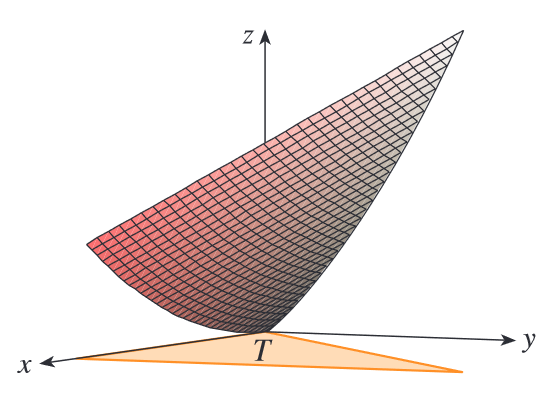
\includegraphics[scale=0.5]{example16-5-1.png}
\end{center}

\section{Triple Integrals}

\subsection*{Definition}
The \textbf{triple integral} of $f$ over the box $B$ is
$$\iiint\limits_B f(x,y,z)\:dV=\lim_{l,m,n\to\infty}\sum_{i=1}^l\sum_{j=1}^m\sum_{k=1}^n
    f(x_{ijk}^*,y_{ijk}^*,z_{ijk}^*)\Delta V$$

\subsection*{Fubini's Theorem for Triple Integrals}
If $f$ is continuous on the rectangular box $B=[a,b]\times[c,d]\times[r,s]$, then
$$\iiint\limits_B f(x,y,z)\:dV=\int_r^s\int_c^d\int_a^b f(x,y,z)\:dx\:dy\:dz$$

\subsection*{Example}
Evaluate $\iiint\limits_E z\:dV$, where $E$ is the solid tetrahedron bounded by the
four planes $x=0$, $y=0$, $z=0$, and $x+y+z=1$.

\subsection*{Solution}
When we set up a triple integral it's wise to draw \textbf{two} diagrams: one of the
solid region $E$ and one of its projection $D$ on the $xy$-plane. The lower boundary
of the tetrahedron is the plane $z=0$ and the upper boundary is the plane $x+y+z=1$,
so we use $u_1(x,y)=$ and $u_2(x,y)=1-x-y$. Notice that the planes $x+y+z=1$ and $z=0$
intersect in the line $x+y=1$ in the $xy$-plane. So the projection of $E$ is the triangular
region and we have
$$E=\{(x,y,z)\:|\:0\leq x\leq 1,\:0\leq y\leq 1-x,\:0\leq z\leq 1-x-y\}$$
This description of $E$ as a type I region enables us to evaluate the integral as follows:
\begin{align*}
    \iiint\limits_E z\:dV & =\int_0^1\int_0^{1-x}\int_0^{1-x-y}z\:dz\:dy\:dx=\int_0^1\int_0^{1-x}\left[\frac{z^2}{2}\right]_{z=0}^{z=1-x-y}dy\:dx  \\
                          & =\frac{1}{2}\int_0^1\int_0^{1-x}(1-x-y^2)\:dy\:dx=\frac{1}{2}\int_0^1\left[-\frac{(1-x-y)^3}{3}\right]_{y=0}^{y=1-x}dx \\
                          & =\frac{1}{6}\int_0^1(1-x)^3\:dx=\frac{1}{6}\left[-\frac{(1-x)^4}{4}\right]_0^1=\frac{1}{24}
\end{align*}

\subsection*{Applications of Triple Integrals}
The case where $f(x,y,z)=1$ for all points in $E$, the triple integral represents the volume of $E$:
$$V(E)=\iiint\limits_E dV$$

\subsection*{Example}
Use a triple integral to find the volume of the tetrahedron $T$ bounded by the planes
$x+2y+z=2$, $x=2y$, $x=0$, and $z=0$.

\subsection*{Solution}
The tetrahedron $T$ and its projection $D$ on the $xy$-plane are shown below. The
lower boundary of $T$ is the plane $z=0$ and the upper boundary is the plane $x+2y+z=2$,
that is, $z=2-x-2y$.
\begin{center}
    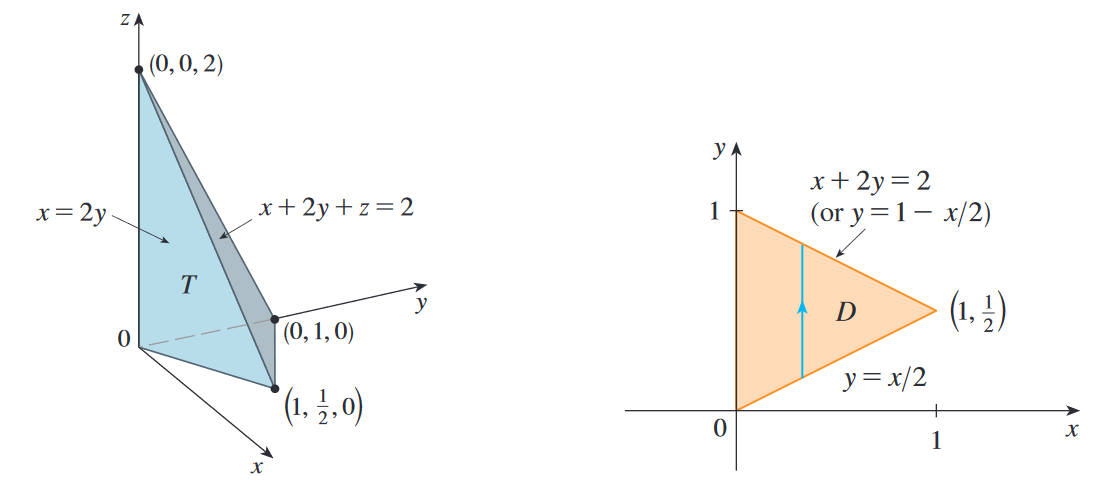
\includegraphics[scale=0.5]{example16-7-1.png}
\end{center}
Therefore, we have
$$V(T)=\iiint\limits_T dV=\int_0^1\int_{x/2}^{1-x/2}\int_0^{2-x-2y}dz\:dy\:dx$$
$$=\int_0^1\int_{x/2}^{1-x/2}(2-x-2y)\:dy\:dx=\frac{1}{3}$$

\section{Triple Integrals in Cylindrical and Spherical Coordinates}

\subsection*{Cylindrical Coordinates}
To convert form cylindrical to rectangular coordinates, we use the equations
$$x=r\cos{\theta} \qquad y=r\sin{\theta} \qquad z=z$$
whereas to convert from rectangular to cylindrical coordinates, we use
$$r^2=x^2+y^2 \qquad \tan{\theta}=\frac{y}{x} \qquad z=z$$

\subsection*{Triple Integration in Cylindrical Coordinates}
$$\iiint\limits_E f(x,y,z)\:dV=\int_\alpha^\beta\int_{h_1(\theta)}^{h_2(\theta)}
    \int_{u_1(r\cos{\theta}, r\sin{\theta})}^{u_2(r\cos{\theta}, r\sin{\theta})}
    f(r\cos{\theta}, r\sin{\theta}, z)\:r\:dz\:dr\:d\theta$$

\subsection*{Example}
A solid $E$ lies within the cylinder $x^2+y^2=1$, below the plane $z=4$, and above
the paraboloid $z=1-x^2-y^2$. The density at any point is proportional to its distance
from the axis of the cylinder. Find the mass of $E$.

\subsection*{Solution}
In cylindrical coordinates the cylinder is $r=1$ and the paraboloid is $z=1-r^2$,
so we can write
$$E=\{(r,\theta,z)\:|\:0\leq\theta\leq 2\pi,\:0\leq r\leq 1,\: 1-r^2\leq z\leq 4\}$$
Since the density at $(x,y,z)$ is proportional to the distance from the $z$-axis, the
density function is
$$f(x,y,z)=K\sqrt{x^2+y^2}=Kr$$
where $K$ is the proportionality constant. Therefore, the mass of $E$ is
$$m=\iiint\limits_E K\sqrt{x^2+y^2}\:dV=\int_0^{2\pi}\int_0^1\int_{1-r^2}^4(Kr)\:r\:dz\:dr\:d\theta$$
$$=\int_0^{2\pi}\int_0^1 Kr^2[4-(1-r^2)]\:dr\:d\theta=K\int_0^{2\pi} d\theta\int_0^1(3r^2+r^4)\:dr$$
$$=2\pi K\left[r^3+\frac{r^5}{5}\right]_0^1=\frac{12\pi K}{5}$$

\subsection*{Spherical Coordinates}
To convert from spherical to rectangular coordinates, we use the eqations
$$x=\rho\sin{\phi}\cos{\theta} \qquad y=\rho\sin{\phi}\sin{\theta} \qquad z=\rho\cos{\phi}$$
Also, the distance formula shows that
$$\rho^2=x^2+y^2+z^2$$

\subsection*{Triple Integration in Spherical Coordinates}
$\iiint\limits_E f(x,y,z)\:dV$
$$=\int_c^d\int_\alpha^\beta\int_a^b f(\rho\sin{\phi}\cos{\theta},
    \rho\sin{\phi}\sin{\theta},\rho\cos{\phi})\:\rho^2\sin{\phi}\:d\rho\:d\theta\:d\phi$$
where E is a spherical wedge given by
$$E=\{(\rho,\theta,\phi)\:|\:a\leq\rho\leq b,\: \alpha\leq\theta\leq\beta,\:c\leq\phi\leq d\}$$

\subsection*{Example}
Evaluate $\iiint\limits_B e^{(x^2+y^2+z^2)^{3/2}}dV$, where $B$ is the unit ball:
$$B=\{(x,y,z)\:|\: x^2+y^2+z^2\leq 1\}$$

\subsection*{Solution}
Since the boundary of $B$ is a sphere, we use spherical coordinates:
$$B=\{(\rho,\theta,\phi)\:|\:0\leq\rho\leq 1,\: 0\leq\theta\leq 2\pi,\:0\leq\phi\leq\pi\}$$
In addition, spherical coordinates are appropriate because
$$x^2+y^2+z^2=\rho^2$$
Thus
$$\iiint\limits_B e^{(x^2+y^2+z^2)^{3/2}}dV=\int_0^\pi\int_0^{2\pi}\int_0^1 e^{(\rho^2)^{3/2}}
    \rho^2\sin{\phi}\:d\rho\:d\theta\:d\phi$$
$$=\int_0^\pi\sin{\phi}\:d\phi\int_0^{2\pi}d\theta\int_0^1\rho^2e^{\rho^3}\:d\rho$$
$$=\left[-\cos{\phi}\right]_0^\pi (2\pi)\left[\frac{1}{3}e^{\rho^3}\right]_0^1=\frac{4}{3}\pi(e-1)$$

\section{Change of Variables in Multiple Integrals}

\subsection*{Example}
A transformation is defined by the equations
$$x=u^2-v^2 \qquad y=2uv$$
Find the image of the square $S=\{(u,v)\:|\:0\leq u\leq 1,\: 0\leq v\leq 1\}$.

\subsection*{Solution}
The transformation maps the boundary of $S$ into the boundary of the image.
So we begin by finding the images of the sides of $S$. The first side, $S_1$,
is given by $v=0$ $(0\leq u\leq 1)$. From the given equations we have $x=u^2$, $y=0$,
and so $0\leq x\leq 1$. Thus $S_1$ is mapped onto the line segment from (0,0) to (1,0)
in the $xy$-plane. The second side, $S_2$, is $u=1$ $(0\leq v\leq 1)$ and, putting
$u=1$ in the given equations, we get
$$x=1-v^2 \qquad y=2v$$
Eliminating $v$, we obtain
$$x=1-\frac{y^2}{4} \qquad 0\leq x\leq 1$$
which is part of a parabola. Similarly, $S_3$ is given by $v=1$ $(0\leq u\leq 1)$, whose
image is the parabolic arc
$$x=\frac{y^2}{4}-1 \qquad -1\leq x\leq 0$$
Finally, $S_4$ is given by $u=0$ $(0\leq v\leq 1)$ whose image is $x=-v^2$, $y=0$,
that is, $-1\leq x\leq 0$. The image of $S$ is the region $R$ bounded by the $x$-axis
and the parabolas given by the two equations we found.

\subsection*{Definition}
The \textbf{Jacobian} of the transformation $T$ given by $x=g(u,v)$ and $y=h(u,v)$ is
$$\pdv{(x,y)}{(u,v)}=
    \begin{vmatrix}
        \dfrac{\partial x}{\partial u} & \dfrac{\partial x}{\partial v} \\[1em]
        \dfrac{\partial y}{\partial u} & \dfrac{\partial y}{\partial v}
    \end{vmatrix}
    =\pdv{x}{u}\pdv{y}{v}-\pdv{x}{v}\pdv{y}{u}$$

\subsection*{Change of Variables in a Double Integral}
Suppose that $T$ is a $C^1$ transformation whose Jacobian is nonzero and that $T$
maps a region $S$ in the $uv$-plane onto a region $R$ in the $xy$-plane. Suppose
that $f$ is continuous on $R$ and that $R$ and $S$ are type I or type II plane regions.
Suppose also that $T$ is one-to-one, except perhaps on the boundary of $S$. Then
$$\iint\limits_R f(x,y)\:dA=\iint\limits_S f(x(u,v),y(u,v))\begin{vmatrix}
        \dfrac{\partial (x,y)}{\partial (y,v)}
    \end{vmatrix}\:du\:dv$$

\subsection*{Example}
Use the change of variables $x=u^2-v^2$, $y=2uv$ to evaluate the integral
$\iint\limits_R y\:dA$ where $R$ is the region bounded by the $x$-axis and the
parabolas $y^2=4-4x$ and $y=4+4x$.

\subsection*{Solution}
$T(S)=R$, where $S$ is the square $[0,1]\times[0,1]$. Indeed, the reason for making
the change of variables to evaluate the integral is that $S$ is a much simpler region
$R$. First we need to compute the Jacobian:
$$\pdv{(x,y)}{(u,v)}=
    \begin{vmatrix}
        \dfrac{\partial x}{\partial u} & \dfrac{\partial x}{\partial v} \\[1em]
        \dfrac{\partial y}{\partial u} & \dfrac{\partial y}{\partial v}
    \end{vmatrix}
    =\begin{vmatrix}
        2u & -2v \\
        2v & 2u
    \end{vmatrix}
    =4u^2+4v^2>0$$
Therefore, by the Change in Variables in a Double Integral,
$$\iint\limits_R y\:dA=\iint\limits_S 2uv \begin{vmatrix}
        \dfrac{\partial (x,y)}{\partial (u,v)}
    \end{vmatrix}\:dA=\int_0^1\int_0^1
    (2uv)4(u^2+v^2)\:du\:dv$$
$$=8\int_0^1\int_0^1(u^3v+uv^3)\:du\:dv=8\int_0^1\left[\frac{1}{4}u^4v+
        \frac{1}{2}u^2v^3\right]_{u=0}^{u=1}dv$$
$$\int_0^1(2v+4v^3)\:dv=\left[v^2+v^4\right]_0^1=2$$
\chapter{Vector Calculus}

\section{Vector Fields}
A vector field in $\mathbb{R}^2$ is a function $F$ that assigns a 2D vector
$f(x,y)$ to each point $(x,y)$ in 0.

Component functions $P$ and $Q$: $F=P\ihat+Q\jhat$

A vector field on $\mathbb{R}^3$ is a function of $F$ that assigns a 3D vector
$f(x,y,z)$ to each point $(x,y,z)$ in $E$.

\subsection*{Example}
Suppose electric charge $Q$ is located at the origin. According to Coulomb's Law,
the electric force excerted at a point $(x,y,z)$ by vector $\vec{x}=\ev{x,y,z}$ is
$$F(x)=\frac{\epsilon qQ}{|\vec{x}|^3}\vec{x}$$
The force is repulsive for like charges and attractive for unlike charges. These
vector fields are known as \textbf{Force field}. Instead of considering the electric
force $F$, physicists often consider the force per unit charge:
$$E(x)=\frac{1}{q}F(x)=\frac{\epsilon Q}{|\vec{x}|^3}x$$

\subsection*{Gradient Fields}
A gradient of $\nabla f$ is defined by:
$$\nabla f(x,y)=f_x(x,y)\ihat+f_y(x,y)\jhat$$

\subsection*{Example}
Find gradient vector of $f(x,y)=x^2y-y^3$.

\textbf{Solution}
$$\nabla f(x,y)=\pdv{f}{x}\ihat +\pdv{f}{y}\jhat=2xy\ihat +(x^2-3y^2)\jhat$$
A vector field is called a \textbf{conservative vector} field if it is the gradient of some
scalar function, that is, if there exists a function $f$ such that $F=\nabla f$.
In this situation, $f$, is a \textbf{potential function} for $F$.

\section{Line Integrals}

\subsection*{Definition}
If $f$ is defined on a smooth curve $C$ given by $\left[x=x(t)\quad y=y(t)\quad
                a\leq t\leq b \right]$, then the line integral of $f$ along curve $C$ is
$$\int_C f(x,y)\:ds=\lim_{n\to\infty}\sum_{i=1}^nf(x_i^*,y_i^*)\Delta s_i$$
if this limit exists.

The following formula can also be used to evaluate a line integral:
$$\int_C f(x,y)\:ds=\int_a^b f(x(t),y(t))\sqrt{(\dv{x}{t})^2+(\dv{y}{t})^2}dt$$

\subsection*{Example}
A wire takes the shape of the semicircle $x^2+y^2=1, y \geq 0$, and is thicker
near its base than near the top. Find the center of mass of the wire if the linear
density at any point is proportional to its distance from the line $y=1$.

\textbf{Solution}
Use parametrization $x=cos\:t$, $y=sin\:t$, $0\leq t\leq\pi$, and find that $ds=dt$.
The linear density is
$$\rho(x,y)=k(1-y)$$
where $k$ is constant, and so the mass of the wire is
$$m=\int_C k(1-y)ds=\int_0^\pi k(1-sin\:t)dt=k[t+cos\:t]_0^\pi=k(\pi-2)$$
we know that the center of mass of the wire is
$$\overline{y}=\frac{1}{m}\int_C y\rho(x,y)ds=\frac{1}{k(\pi -2)}\int_C yk(1-y)ds$$
$$=\frac{1}{\pi-2}\int_0^\pi(sin\:t-sin^2\:t)dt=\frac{1}{\pi-2}\left[-cos\:t-\frac{1}{2}t+
                \frac{1}{4}sin\:2t\right]_0^\pi=\frac{4-\pi}{2(\pi-2)}$$
By symmetry we see that $\overline{x}=0$, so the center of mass is
$$\left(0, \frac{4-\pi}{2(\pi-2)}\right)\approx(0, 0.38)$$

The line integral with respect to arc length:
$$\int_C f(x,y)\:dx=\int_a^b f(x(t),t(t))\:x'(t)\:dt$$
$$\int_C f(x,y)\:dy=\int_a^b f(x(t),t(t))\:y'(t)\:dt$$
When setting up a line integral, it is often difficult to think of a parametric
representation for a curve. It's useful to remember that a vector representation
of the line segment that starts at $\textbf{r}_0$ and ends at $\textbf{r}_1$ is:
$$\textbf{r}(t)=(1-t)\textbf{r}_0+t\textbf{r}_1\qquad 0\leq t\leq 1$$
A given parametrization $x=x(t)$, $y=y(t)$, $a\leq t\leq b$, determines an
\textbf{orientation} of a curve $C$, with the positive direction corresponding to
increasing values of the parameter $t$.

If $-C$ denotes the curve of the same points as $C$ but with the opposite orientation,
then we have:
$$\int_{-C}f(x,y)\:dx=-\int_Cf(x,y)\:dx\qquad\int_{-C}f(x,y)\:dy=-\int_Cf(x,y)\:dy$$

\subsection*{Line Integrals in Space}
Suppose that $C$ is now a smooth curve. We define the line integral along $C$
(with respect to arc length) in a manner similar to that for plane curves:
$$\int_Cf(x,y,z)\:ds=\int_a^bf(x(t),y(t),z(t))\sqrt{\left(\dv{x}{t}\right)^2+
                \left(\dv{y}{t}\right)^2+\left(\dv{z}{t}\right)^2}dt$$
The integral can also be written as:
$$\int_a^bf(\textbf{r}(t))|\textbf{r}'(t)|\:dt$$

\subsection*{Example}
Evaluate $\int_Cysin\:z\:ds$, where $C$ is the circular helix given by $x=cos\:t$,
$y=sin\:t$, $z=t$, $0\leq t\leq 2\pi$.

\subsection*{Solution}
\begin{align*}
        \int_Cysin\:z\:ds & =\int_0^{2\pi}(sin\:t)sin\:t\sqrt{\left(\dv{x}{t}\right)^2+\left(\dv{y}{t}\right)^2+\left(\dv{z}{t}\right)^2}dt \\
                          & =\int_0^{2\pi}sin^2t\sqrt{sin^2t+cos^2t+1}\:dt=\sqrt{2}\int_0^{2\pi}\frac{1}{2}(1-cos\:2t)\:dt                  \\
                          & =\frac{\sqrt{2}}{2}\left[t-\frac{1}{2}sin\:2t\right]_0^{2\pi}=\sqrt{2}\pi
\end{align*}

\subsection*{Line Integrals of Vector Fields}
$$W=\int_C\textbf{F}(x,y,z)\cdot\textbf{T}(x,y,z)\:ds=\int_C\textbf{F}\cdot\textbf{T}\:ds$$
Work is the line integral with respect to arc length of the tangetial component
for the force.

\subsection*{Definition}
Let $F$ be a continous vector field defined on a smooth curve $C$ given by a vector
function $\textbf{r}(t)$, $a\leq t\leq b$. Then the \textbf{line integral of $F$
        along $C$} is
$$\int_C\textbf{F}\cdot d\textbf{r}=\int_a^b\mathbf{F(r}(t))\cdot\textbf{r}'(t)\:dt=\int_C\mathbf{F\cdot T}\:ds$$

\subsection*{Example}
Find the work done by the force field $\textbf{F}(x,y)=x^2\ihat-xy\jhat$ in moving a
particle along the quarter-circle $\textbf{r}(t)=cos\:t\ihat+sin\:t\jhat$,
$0\leq t\leq\pi/2$.

\textbf{Solution} \\
Since $x=cos\:t$ and $y=sin\:t$, we have
$$\mathbf{F(r}(t))=cos^2t\ihat-cos\:tsin\:t\jhat$$
$$\textbf{r}'(t)=-sin\:t\ihat+cos\:t\jhat$$
Therefore the work done is:
$$\int_C\textbf{F}\cdot d\textbf{r}=\int_0^{\pi/2}\mathbf{F(r}(t))\cdot\textbf{r}'(t)\:dt=
        \int_0^{\pi/2}(-2cos^2t\:sin\:t)\:dt=\left[2\frac{cos^3t}{3}\right]_0^{\pi/2}=-\frac{2}{3}$$

\section{The Fundamental Theorem for Line Integrals}

The Fundamental Theorem of Calculus is:
$$\int_a^b F'(x)\:dx=F(B)-F(a)$$

\subsection*{Theorem}
Let $C$ be a smooth curve given by the vector function $r(t)$, $a\leq t\leq b$.
Let $f$ be a differentiable functino of two or three variables whose gradient vector
$\nabla f$ is continous.
$$\int_C \nabla f\cdot dr=f(r(b))-f(r(a))$$

\subsection*{Proof}
Using the line integral, we have
\begin{align*}
        \int_C \nabla f\cdot dr & =\int_a^b\nabla f(r(t))\cdot r'(t)\:dt                                                   \\
                                & =\int_a^b\left(\pdv{f}{x}\pdv{x}{t}+\pdv{f}{y}\pdv{y}{t}+\pdv{f}{z}\pdv{z}{t}\right)\:dt \\
                                & =\int_a^b \frac{d}{dt} f(r(t))\:dt                                                       \\
                                & =f(r(b))-f(r(a))
\end{align*}

\subsection*{Independence of Path}
If $F$ is a continous vector field with domain $D$, we say that the line integral
$\int_c F\cdot dr$ is independent of path if $\int_{C_1}F\cdot dr=\int_{C_2}F\cdot dr$
for any two paths $C_1$ and $C_2$ in $D$ that have the same initial and terminal paths.

A curve is called closed if $r(b)=r(a)$.

\subsection*{Theorem}
$\int_C F\cdot dr$ is independent of path in $D$ if and only if $\int_C F\cdot dr=0$
for every closed path $C$ in $D$.

\subsection*{Proof}
$$\int_C F\cdot dr=\int_{C_1} F\cdot dr+\int_{C_2} F\cdot dr=\int_{C_1} F\cdot dr-\int_{-C_2} F\cdot dr=0$$
Conversely, if that is true, do the same thing backwards to prove it is closed.

$D$ is open $\to$ for every point $P$ in $D$ there is no disk with center $P$ that
lies entirely on $D$.

$D$ is connected $\to$ any two points in $D$ can be joined by a path in $D$.

\subsection*{Theorem}
$F$ is a vector field that is continous in an open connected region in $D$. If
$\int_C F\cdot dr$ is independent of path in $D$, then $F$ is a conservative vector
field in $D$ where a function $f$ that $\nabla f=F$ exist.

\subsection*{Theorem}
If $F(x,y)+P(x,y)\ihat+Q(x,y)\jhat$ is a conservative vector field, where $P$ and $Q$
have continous first-order partial derivatives on a domain $D$, then through $D$ we have
$$\pdv{P}{y}=\pdv{Q}{x}$$

\subsection*{Theorem}
Let $F+P\ihat + Q\jhat$ be a vector field on an open simply-connected region $D$.
Supposed that $P$ and $Q$ have continous first-order derivatives and
$\pdv{P}{y}=\pdv{Q}{x}$ throughout $D$. Then $F$ is conservative.

\subsection*{Example}
Determine whether or not $F(x,y)=(x,y)\ihat+(x,z)\jhat$ is conservative.

\subsection*{Solution}
Let $P(x,y)=x-y$ and $Q(x,y)=x-z$
$$\text{then} \qquad \pdv{P}{y}=-1 \qquad \pdv{Q}{x}=1$$
since $\pdv{P}{y}\neq\pdv{Q}{x}$, $F$ is not conservative.

\section{Green's Theorem}
Green's Theorem gives the relationship between a line integral around a simpled
curve $C$ and a double integral over the plane region $D$ bounded by $C$.

\subsection*{Green's Theorem}
Let $C$ be a positively oriented, piecewise-smooth, simple closed curve in the plane
and let $D$ be the region bounded by $C$. If $P$ and $Q$ have continous partial derivatives
on an open region that contains $D$, then
$$\int\_C P\:dx+Q\:dy=\iint\limits_D\left(\pdv{Q}{x}-\pdv{P}{y}\right)\:dA$$

\subsection*{Proof}
For the case in with $D$ is a simple region
\begin{enumerate}
        \item[] $D=\{(x,y)\:|\:a\leq x\leq b,\:g_1(x)\leq y\leq g_2(x)\}$
        \item[] $\iint\limits_D \pdv{P}{y}\:dA=\int_a^b\int_{g_1(x)}^{g_2(x)}\pdv{P}{y}(x,y)\:dy\:dx=
                      \int_a^b \left[P(x,g_2(x))-P(x,g_1(x))\right]\:dx$
        \item[] $\int_{C_1} P(x,y)\:dx=\int_a^b P(x,g(1(x)))\:dx$
        \item[] $\int_{C_3} P(x,y)\:dx=-\int_{-C_3} P(x,y)\:dx=-\int_a^b P(x,g_2(x))\:dx$
        \item[] $\int_{C_2} P(x,y)\:dx=0=\int_{C_4} P(x,y)\:dx$
        \item[] $\int_C P(x,y)\:dx=\int_{C_1} P(x,y)\:dx+\int_{C_2} P(x,y)\:dx+\int_{C_3} P(x,y)\:dx$
        \item[] $+\int_{C_4} P(x,y)\:dx$
        \item[] $\int_a^b P(x,g_1(x))\:dx-\int_a^b P(x,g_2(x))\:dx$
        \item[] $\int_C P(x,y)\:dx=-\iint\limits_D \pdv{P}{y}\:dA$
\end{enumerate}

\subsection*{Example}
Evaluate $\oint_C (3y-c^{\sin{x}})\:dx+(7x+\sqrt{y^4+1})\:dy$, where $C$ is the circle
$x^2+y^2=9$.

\subsection*{Solution}
The region $D$ bounded by $C$ is the disk $x^2+y^2\leq 9$ so let's change to polar
coordinates after applying Green's Theorem:
$$\oint_C (3y-c^{\sin{x}})\:dx+(7x+\sqrt{y^4+1})\:dy$$
$$=\iint\limits_D \left[\frac{\partial}{\partial x}(7x+\sqrt{y^4+1})-\frac{\partial}{\partial y}
                (3y-e^{\sin{x}})\right]\:dA$$
$$=\int_0^{2\pi}\int_0^3 (7-3)\:r\:dr\:d\theta=4\int_0^{2\pi}d\theta\int_0^3r\:dr=36\pi$$

The Green's Theorem gives the following formulas for the area of $D$:
$$A=\oint_C x\:dy=-\oint_C y\:dx=\frac{1}{2}\oint_C x\:dy-y\:dx$$

\subsection*{Example}
Find the area enclosed by the ellipse $\cfrac{x^2}{a^2}+\cfrac{y^2}{b^2}=1$.

\subsection*{Solution}
The ellipse has parametric equations $x=a\cos{t}$ and $y=b\sin{t}$, where $0\leq t\leq 2\pi$.
Using the formula for area from above, we have
$$A=\frac{1}{2}\int_C x\:dy-y\:dx$$
$$\frac{1}{2}\int_0^{2\pi}(a\cos{t})(b\cos{t})\:dt-(b\sin{t})(-a\sin{t})\:dt$$
$$\frac{ab}{2}\int_0^{2\pi}dt=\pi ab$$

\section{Curl and Divergence}

\subsection*{Curl}
If $F+P\ihat+Q\jhat+R\khat$ is a vector field on $\mathbb{R}^3$ and the partial
derivatives of $P$, $Q$, and $R$ all exist, then the \textbf{curl} of $F$ is the
vector field on $\mathbb{R}^3$ defined by
$$\text{curl F}=\left(\pdv{R}{y}-\pdv{Q}{z}\right)\ihat+\left(\pdv{P}{z}-\pdv{R}{x}\right)\jhat+
        \left(\pdv{Q}{x}-\pdv{P}{y}\right)\khat$$
$$\text{or} \qquad \text{curl F}=\nabla \times F$$

\subsection*{Example}
$F(x,y,z)=xz\ihat+xyz\jhat-y^2\khat$, find curl F.

\subsection*{Solution}
\begin{align*}
        \text{curl F} & =\nabla \times F=\begin{vmatrix}
                \ihat                        & \jhat                        & \khat                        \\
                \dfrac{\partial}{\partial x} & \dfrac{\partial}{\partial y} & \dfrac{\partial}{\partial z} \\
                xz                           & xyz                          & -y^2
        \end{vmatrix}                                             \\
                      & =\left[\frac{\partial}{\partial y}(-y^2)-\frac{\partial}{\partial z}(xyz)\right]\ihat-
        \left[\frac{\partial}{\partial x}(-y^2)-\frac{\partial}{\partial z}(xz)\right]                         \\
                      & +\left[\frac{\partial}{\partial x}(xyz)-\frac{\partial}{\partial y}(xz)\right]         \\
                      & =(-2y-xy)\ihat-(0-x)\jhat+(yz-0)\khat                                                  \\
                      & =-y(2+x)\ihat+x\jhat+yz\khat
\end{align*}

\subsection*{Theorem}
If $F=P\ihat+Q\jhat+R\khat$ is a vector field on $\mathbb{R}^3$ and $P$, $Q$, and $R$
have continous second-order partial derivatives, then
$$\text{div curl F}=0$$

\subsection*{Proof}
Using the definitions of divergence and curl, we have
$$\text{div curl F}=\nabla\cdot(\nabla\times \textbf{F})$$
$$=\frac{\partial}{\partial x}\left(\pdv{R}{y}-\pdv{Q}{z}\right)+
        \frac{\partial}{\partial y}\left(\pdv{P}{z}-\pdv{R}{x}\right)+
        \frac{\partial}{\partial z}\left(\pdv{Q}{x}-\pdv{P}{y}\right)$$
$$=\pdv{R}{x}{y}-\pdv{Q}{x}{z}+\pdv{P}{y}{z}-\pdv{R}{y}{x}+\pdv{Q}{z}{x}-\pdv{P}{z}{y}$$
$$=0$$

\subsection*{Vector Forms of Green's Theorem}
$F=P\ihat+Q\jhat$, its line integral is:
$$\oint_C F\cdot dr=\oint_C P\:dx + Q\:dy$$
and its curl is:
$$\text{curl F}=\begin{vmatrix}
                \ihat     & \jhat     & \khat     \\
                \pdv{}{x} & \pdv{}{y} & \pdv{}{z} \\
                P(x,y)    & Q(x,y)    & 0
        \end{vmatrix}=
        \left(\pdv{Q}{x}-\pdv{P}{y}\right)\khat$$
Therefore
$$\text{curl F}\cdot \khat = \left(\pdv{Q}{x}-\pdv{P}{y}\right)\khat\cdot\khat=\pdv{Q}{x}-\pdv{P}{y}$$
and we can now rewrite the equation in Green’s Theorem in the vector form
$$\oint_C F\cdot dr=\iint\limits_D (\text{curl F})\cdot\khat\:dA$$

A similar function involving the \textbf{normal} component of $F$:
$$\oint_C F\cdot n\:ds=\iint\limits_D \text{div F}(x,y)\:dA$$

\section{Parametric Surfaces and Their Areas}

\subsection*{Parametric Surfaces}
The set of all points $(x,y,z)$ in $\mathbb{R}^3$ such that
$$x=x(u,v) \qquad y=y(u,v) \qquad z=z(u,v)$$
and $(u,v)$ varies through $D$, is called a \textbf{parametric surface} $S$.

\subsection*{Example}
Identify and sketch the surface with vector equation
$$r(u,v)=2\cos{u}\ihat + v\jhat + 2\sin{u}\khat$$

\subsection*{Solution}
The parametric equations for this surface are
$$x=2\cos{u}\qquad y=v \qquad z=2\sin{u}$$
So for any point $(x,y,z)$ on the surface, we have
$$x^2+z^2=4\cos^2{u}+4\sin^2{u}=4$$
Since $y=v$ and no restriction is placed on $v$, the surface  is a circular cylinder with radius 2 whose axis is the $y$-axis.
\begin{center}
        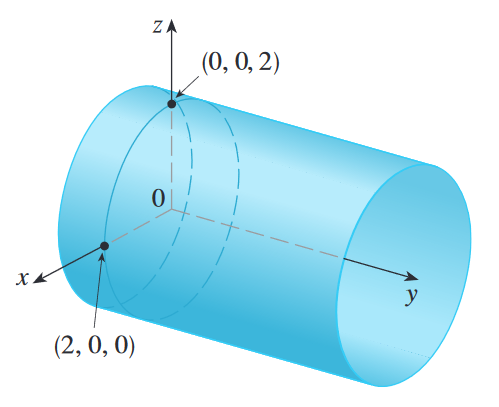
\includegraphics[scale=0.5]{example17-6-1.png}
\end{center}

\subsection*{Tangent Planes}
The tangent vector to $C_1$ at $P_0$ is obtained by taking the partial derivative
of $r$ with respect to $v$:
$$r_v=\pdv{x}{v}(u_0,v_0)\ihat+\pdv{y}{v}(u_0,v_0)\jhat+\pdv{z}{v}(u_0,v_0)\khat$$
Same thing fo $r_u$ but $\partial v$ changes to $\partial u$.

If $r_u\times r_v$ is not 0, the surface $S$ is called smooth (has no corners).
For a smooth surface, the \textbf{tangent plane} is the plane that contains $r_u$ and
$r_v$, and the vector $r_u\times r_v$ is a normal vector to the tangent plane.

\subsection*{Example}
Find the tangent plane to the surface with parametric equations $x=u^2$, $y=v^2$,
$z=u+2v$ at the point (1, 1, 3).

\subsection*{Solution}
We first compute the tangent vectors:
$$r_u=\pdv{x}{u}\ihat+\pdv{y}{u}\jhat+\pdv{z}{u}\khat=2u\ihat+\khat$$
$$r_v=\pdv{x}{v}\ihat+\pdv{y}{v}\jhat+\pdv{z}{v}\khat=2v\jhat+\khat$$
Thus a normal vector to the tangent plane is
$$r_u\times r_v=\begin{vmatrix}
                \ihat & \jhat & \khat \\
                2u    & 0     & 1     \\
                0     & 2v    & 2
        \end{vmatrix}=-2v\ihat-4u\jhat+4uv\khat$$
The point (1, 1, 3) corresponds to the parameter values $u=1$ and $v=1$, so the normal vector there is
$$-2\ihat-4\jhat+4\khat$$
Therefore an equation of the tangent plane at (1, 1, 3) is
$$-2(x-1)-4(y-1)+4(z-3)=0$$
$$\text{or} \qquad x+2y-2z+3=0$$

\subsection*{Surface Area}
$$A(S)=\iint\limits_D \sqrt{1+\left(\pdv{z}{x}\right)^2+\left(\pdv{z}{y}\right)^2}\:dA$$

\subsection*{Example}
Find the area of the part of the paraboloid $z=x^2+y^2$ that lies under the plane $z=9$.

\subsection*{Solution}
The plane intersects the paraboloid in the circle $x^2+y^2=9$, $z=9$. Therefore the
given surface lies above the disk $D$ with center the origin and radius 3.
\begin{align*}
        A & =\iint\limits_D \sqrt{1+\left(\pdv{z}{x}\right)^2+\left(\pdv{z}{y}\right)^2}\:dA \\
          & =\iint\limits_D\sqrt{1+(2x)^2+(2y)^2}\:dA                                        \\
          & =\iint\limits_D\sqrt{1+4(x^2+y^2)}\:dA
\end{align*}
Converting to polar coordinates, we obtain
\begin{align*}
        A & =\int_0^{2\pi}\int_0^3 \sqrt{1+4r^2}\:r\:dr\:d\theta=\int_0^{2\pi}d\theta\int_0^3r\sqrt{1+4r^2}\:dr  \\
          & =\left[2\pi\left(\frac{1}{8}\right)\frac{2}{3}(1+4r^2)^{3/2}\right]_0^3=\frac{\pi}{6}(37\sqrt{37}-1)
\end{align*}

\section{Surface Integrals}
Surface integral of $f$ over the surface $S$:
$$\iint\limits_S f(x,y,z)\:dS=\iint\limits_D f(x,y,g(x,y))\sqrt{\left(\pdv{z}{x}\right)^2+
                \left(\pdv{z}{y}\right)^2+1}\:dA$$

\subsection*{Example}
Evaluate $\iint\limits_S y\:dS$, where $S$ is the surface $z=x+y^2$, $0\leq x\leq 1$,
$0\leq y\leq 2$.

\subsection*{Solution}
Since
$$\pdv{z}{x}=1 \qquad \text{and} \qquad \pdv{z}{y}=2y$$
\begin{align*}
        \iint\limits_S y\:dS & =\iint\limits_D y\sqrt{1+\left(\pdv{z}{x}\right)^2+\left(\pdv{z}{y}\right)^2}\:dA                \\
                             & =\int_0^1\int_0^2 y\sqrt{1+1+4y^2}\:dy\:dx                                                       \\
                             & =\int_0^1 dx\sqrt{2}\int_0^2 y\sqrt{1+2y^2}\: dy                                                 \\
                             & =\left[\sqrt{2}\left(\frac{1}{4}\right)\frac{2}{3}(1+2y^2)^{3/2}\right]_0^2=\frac{13\sqrt{2}}{3}
\end{align*}

\subsection*{Surface Integrals of Vector Fields}
The mass of a fluid crossing $S_{ij}$ in the direction of the normal $n$ per unit
time by the quantity
$$(pv\cdot n)A(S_{ij})$$
where $p$, $v$, and $n$ are evaluated at some point on $S_{ij}$.
$$\iint\limits_S pv\cdot n\:dS=\iint\limits_S p(x,y,z)v(x,y,z)\cdot n(x,y,z)\:dS$$
is the rate of flow through $S$.

If we write $F=pv$, then $F$ is also a vector field on $\mathbb{R}^3$ and the integral above becomes
$$\iint\limits_S F\cdot n\:dS$$

\subsection*{Definition}
If  $F$ is a continuous vector field defined on an oriented surface $S$ with unit normal
vector $n$, then the \textbf{surface integral of $F$ over $S$} is
$$\iint\limits_S F\cdot dS=\iint\limits_S F\cdot n\:dS$$
This integral is also called the \textbf{flux} of $F$ across F.

It can also be written as:
$$\iint\limits_S F\cdot dS=\iint\limits_D\left(-P\pdv{g}{x}-Q\pdv{g}{y}+R\right)\:dA$$

\subsection*{Example}
Evaluate $\iint_S F\cdot dS$, where $F(x,y,z)=y\ihat+x\jhat+z\khat$ and $S$ is the
boundary of the solid region $E$ enclosed by the paraboloid $z=1-x^2-y^2$ and the plane $z=0$.

\subsection*{Solution}
$$P(x,y,z)=y \qquad Q(x,y,z)=x \qquad R(x,y,z)=z=1-x^2-y^2$$
$$\pdv{g}{x}=-2x \qquad \text{and} \qquad \pdv{g}{y}=-2y$$
\begin{align*}
        \iint\limits_{S_1} F\cdot dS & =\iint\limits_D\left(-P\pdv{g}{x}-Q\pdv{g}{y}+R\right)\:dA                                      \\
                                     & =\iint\limits_D[-y(-2x)-x(-2y)+1-x^2-y^2]\:dA                                                   \\
                                     & =\iint\limits_D(1+4xy-x^2-y^2)\:dA                                                              \\
                                     & =\int_0^{2\pi}\int_0^1(1+4r^2\cos{\theta}\sin{\theta}-r^2)\:r\:dr\:d\theta                      \\
                                     & =\int_0^{2\pi}\int_0^1(r-r^3+4r^3\cos{\theta}\sin{\theta})\:dr\:d\theta                         \\
                                     & =\int_0^{2\pi}(\frac{1}{4}+\cos{\theta}\sin{\theta})\:d\theta=\frac{1}{4}(2\pi)+0=\frac{\pi}{2}
\end{align*}

The disk $S_2$ is oriented downward, so its unit normal vector is $n=-\khat$ and we have
$$\iint\limits_{S_2} F\cdot dS=\iint\limits_{S_2} F\cdot(-\khat)\:dS=\iint\limits_D
        (-z)\:dA=\iint\limits_D 0\:dA=0$$
$$\iint\limits_S F\cdot dS=\iint\limits_{S_1}F\cdot dS+\iint\limits_{S_2}F\cdot dS=
        \frac{\pi}{2}+0=\frac{\pi}{2}$$

\section{Stokes Theorem}

\subsection*{Stokes Theorem}
Let  $S$ be an oriented piecewise-smooth surface that is bounded by a simple, closed,
piecewise-smooth boundary curve $C$ with positive orientation. Let $F$ be a vector
field whose components have continuous partial derivatives on an open region in
$\mathbb{R}^3$ that contains $S$. Then
$$\int_C F\cdot dr=\iint\limits_S \text{curl F}\cdot dS$$

\subsection*{Proof}
\begin{align*}
        \oint F\cdot dr & =\iint(\nabla\times\bar{F})\cdot dA=\int(F_xdx+F_ydy+F_zdz)                                                  \\
                        & =\int(\int dF_xdx)+\int(\int dF_ydy)+\int(\int dF_zdz)                                                       \\
                        & =\int(\int \pdv{F_x}{y}dy+\pdv{F_x}{z}dz)dx+\int(\pdv{F_y}{x}dx+\pdv{F_y}{z}dz)dy                            \\
                        & +\int(\pdv{F_z}{x}dx+\pdv{F_z}{y}dy)dz)                                                                      \\
                        & \text{order of integration matters: }dx\times dy=-dy\times dx                                                \\
                        & =\int(\int-\pdv{F_x}{y}dxdy+\pdv{F_x}{z}dzdx)+(\int\pdv{F_y}{x}dxdy-\pdv{F_y}{z}dydz)                        \\
                        & +\int(-\pdv{F_z}{x}dzdx+\pdv{F_z}{y}dydz)                                                                    \\
                        & =\int(\pdv{F_z}{y}-\pdv{F_y}{z})dydz+\int(\pdv{F_y}{z}-\pdv{F_z}{x})dzdx+\int(\pdv{F_y}{x}-\pdv{F_x}{y})dxdy \\
                        & =\int(\int \nabla\times F)_x dA_x + (\int \nabla\times F)_y dA_y + (\int \nabla\times F)_z dA_z              \\
                        & =\iint(\nabla\times\bar{F}\cdot d\bar{A})
\end{align*}

\subsection*{Example}
Use Stokes’ Theorem to compute the integral $\iint_S \text{curl F}\cdot dS$, where
$F(x,y,z)=xz\ihat+yz\jhat+xy\khat$ and $S$ is the part of the sphere $x^2+y^2+z^2=4$
that lies inside the cylinder $x^2+y^2=1$ and above the $xy$-plane.

\subsection*{Solution}
To find the boundary curve $C$ we solve the equations $x^2+y^2+z^2=4$ and $x^2+y^2=1$.
Subtracting, we get $z^2=3$ and so $z=\sqrt{3}$. Thus $C$ is the circle given by the
equations $x^2+y^2=1$, $z=\sqrt{3}$. A vector equation of $C$ is
$$r(t)=\cos{t}\ihat+\sin{t}\jhat+\sqrt{3}\khat \qquad 0\leq t\leq 2\pi$$
$$r'(t)=-\sin{t}\ihat+cos{t}\jhat$$
$$F(r(t))=\sqrt{3}\cos{t}\ihat+\sqrt{3}\sin{t}\jhat+\cos{t}\sin{t}\khat$$
Therefore, by Stokes' Theorem
$$\iint\limits_S \text{curl F}\cdot dS=\int_C F\cdot dr=\int_0^{2\pi} F(r(t))\cdot r'(t)\:dt$$
$$=\int_0^{2\pi}(-\sqrt{3}\cos{t}\sin{t}+\sqrt{3}\sin{t}\cos{t})\:dt$$
$$\sqrt{3}\int_0^{2\pi}0\:dt=0$$

\section{Divergence Theorem}

\subsection*{The Divergence Theorem}
Let $E$ be a simple solid region and let $S$ be the boundary surface of $E$,
given with positive (outward) orientation. Let $F$ be a vec­tor field whose
component functions have continuous partial derivatives on an open region that
contains $E$. Then
$$\iint\limits_S F\cdot dS=\iiint\limits_E \text{div F}\:dV$$

\subsection*{Proof}
\begin{align*}
        \oiint \bar{F}\cdot d\bar{S} & =\iint(F_xdA_x+F_ydA_y+F_zdA_z)                                    \\
                                     & =\iint F_xdydz + F_ydzdx + F_zdxdy                                 \\
                                     & =\iiint (\pdv{F_x}{x}dxdydz+\pdv{F_y}{y}dydzdx+\pdv{F_z}{z}dzdxdy) \\
                                     & =\iiint \nabla \bar{F}\:dV
\end{align*}

\subsection*{Example}
Find the flux of the vector field $F(x,y,z)=z\ihat+y\jhat+x\khat$ over the unit
sphere $x^2+y^2+z^2=1$.

\subsection*{Solution}
First we compute the divergence of $F$:
$$\text{div F}=\pdv{}{x}(z)+\pdv{}{y}(y)+\pdv{}{z}(x)=1$$
The unit sphere $S$ is the boundary of the unit ball $B$ given by $x^2+y^2+z^2\leq 1$.
Thus the Divergence Theorem gives the flux as
$$\iint\limits_S F\cdot dS = \iiint\limits_B 1\:dV=V(B)=\frac{4}{3}\pi(1)^3=\frac{4\pi}{3}$$
\chapter{Second-Order Differential Equations}

\section{Second-Order Differential Equations}
A second-order differential equation has the form
$$P(x)\frac{d^y}{dx^2}+Q(x)\frac{dy}{dx}+R(x)y=G(x)$$
If given in the form
$$ay''+by'+cy=0$$
Replacing $y''$ with $r^2$, $y'$ with $r$, and $y$ with 1 lets us solve the
equation using the auxiliary equation
$$ar^2+br+c=0$$
\begin{description}
    \item [Case 1:] $b^2-4ac>0 \qquad y=c_1e^{r_1x}+c_2e^{r_2x}$
    \item [Case 2:] $b^2-4ac=0 \qquad y=c_1e^{r_1x}+c_2xe^{r_2x}$
    \item [Case 3:] $b^2-4ac<0 \qquad y=e^{\alpha x}(c_1cos\:\beta x+c_2sin\: \beta x)$
          \subitem $\alpha = \frac{-b}{(2a)}$ and $\beta = \frac{\sqrt{4ac-b^2}}{(2a)}$
\end{description}

\subsection*{Example}
Solve the equation $y''+y'-6y=0$ with the initial values $y(0)-1$, $y'(0)=0$

\subsection*{Solution}
The auxiliary equation is
$$r^2+r+6=(r-2)(r+3)=0$$
So the solution is
$$y=c_1e^{2x}+c_2e^{-3x}$$
Differentiating this, we get
$$y'=2c_1e^{2x}-3c_2e^{-3x}$$
Satisfying initial conditions
$$y(0)=c_1+c_2=1$$
$$y'(0)=2c_1-3c_2=0$$
$$c_1=\frac{3}{5} \qquad c_2=\frac{2}{5}$$
Giving us the solution
$$y=\frac{3}{5}e^{2x}+\frac{2}{5}e^{-3x}$$

\section{Nonhomogenous Linear Equations}

\subsection*{Method of Undetermined Coefficients}
If the differential equation is given in the form $ay''+by'+cy=G(x)$, then the solution
is given by
$$y(x)=y_p(x)+y_c(x)$$
Where $y_c(x)$ is the general solution and $y_p(x)$ is the particular solution.

\subsection*{Proof}
\begin{itemize}
    \item[] $a(y - y_p)'' + b(y - y_p)' + c(y - y_p) = ay'' - ay_p'' + by' - by_p' + cy - cy_p$
    \item[] $a(y - y_p)'' + b(y - y_p)' + c(y - y_p) = (ay'' + by' + cy) - (ay_p'' + by_p' + cy_p)$
    \item[] $a(y - y_p)'' + b(y - y_p)' + c(y - y_p) = g(x) - g(x) = 0$
\end{itemize}

\subsection*{Example}
Solve the equation $y''+y'-2y=x^2$

\subsection*{Solution}
The auxiliary equation becomes
$$r^2+r-2=(r-1)(r+2)=0$$
which gives a complementary solution of
$$y_c=c_1e^x+c_2e^{-2x}$$
Since $G(x)$ is a polynomial of the 2nd degree, this gives a particular solution
\begin{itemize}
    \item[] $y_p(x)=Ax^2+Bx+C$
    \item[] $y_p'(x)=2Ax+B$
    \item[] $y_p''(x)=2A$
\end{itemize}
Substituting into the original differential equation gives
$$(2A) + (2Ax + B) - 2(Ax^2 + Bx + C) = x^2$$
$$A=-\frac{1}{2} \qquad B=-\frac{1}{2} \qquad C=-\frac{3}{4}$$
which gives the particular solution
$$y_p(x)=-\frac{1}{2}x^2-\frac{1}{2}x-\frac{3}{4}$$
so the final solution is
$$y = c_1e^x + c_2e^{-2x} +  -\frac{1}{2} x^2 - \frac{1}{2} x - \frac{3}{4}$$

\subsection*{Method of Variation of Parameters}
If we have already solved the homogeneous equation $ay''+by'+cy=0$ in the form
$$y(x)=c_1y_1(x)+c_2y_2(x)$$
We can replace the constants and write this with an arbitrary function $u(x)$
$$y_p(x)=u_1(x)y_1(x)+u_2(x)y_2(x)$$
$$y_p'(x)=(u_1'y_1+u_2'y_2)+(u_1y_1'+u_2y_2')$$

\subsection*{Example}
Solve the equation $y''+y=tan\:x$, $0<x<\pi/2$

\subsection*{Solution}
Solving for the complementary equation gives us
$$r^1+1=0$$
$$y_c(x)=c_1sin\:x+c_2cos\:x$$
Using variation of parameters means we need a solution of the form
\begin{itemize}
    \item[] $y_p(x)=u_1(x)sin\:x+u_2(x)cos\:x$
    \item[] $y_p'(x)=(u_1'sin\:x+u_2'cos\:x)+(u_1sin\:x+u_2cos\:x)$
    \item[] $y_p''(x)=u_1'cos\:x-u_2'sin\:x-u_1sin\:x-u_2cos\:x$
\end{itemize}
To get a solution we need
$$y_p''+y_p=u_1'cos\:x-u_2'sin\:x=tan\:x$$
$$u_1'(sin^2x+cos^2x)=cos\:x\:tan\:x$$
$$u_1'=sin\:x \qquad u_1(x)=-cos\:x$$
Solving for $u_2$ gives
$$u_2'(x)=-\frac{sin\:x}{cos\:x} \qquad u_1'(x)=cos\:x-sec\:x$$
$$u_2(x)=sin\:x-lin(sec\:x+tan\:x)$$
Therefore
$$y_p(x)=-cos\:x\:ln(sec\:x+tan\:x)$$
$$y(x)=c_1sin\:x+c_2cos\:x-cos\:x\:ln(sec\:x+tan\:x)$$

\section{Applications of Second-Order Differential Equations}

Vibrating strings follow a second-order differential equation by satisfying
Newton's second law
$$m\frac{d^2x}{dy^2}=-kx$$
The general solution can be written as
$$x(t)=c_1cos\:wt+c_2sin\:wt$$
or
$$x(t)=Acos(wt+\delta)$$
Where
$$w=\sqrt{k/m}$$
$$A=\sqrt{c_1^2+c_2^2}$$
$$cos\:\delta =\frac{c_1}{A} \qquad sin\:\delta = -\frac{c_2}{A}$$
Damped vibrations in a string are subjected to a frictional force but still satisfies
a second-order differential equation
$$m\frac{d^2x}{dy^2}+c\frac{dy}{dx}+kx=0$$
In electrical circuits, voltage drop across resistors, inductors and conductors
must be equal to the supplied voltage, but since $I = \frac{dQ}{dt}$, this turns into a
second-order differential equation
$$L\frac{d^2Q}{dt^2}+R\frac{dQ}{dt}+Q/C=E(t)$$

\subsection*{Example}
A spring with a mass of 2kg has a natural length of 0.5m. A force of 25.6 N
is required to maintain it stretched to a length of 0.7m. If the spring is
stretched to a length of 0.7m and then released with initial velocity 0, find
the position of the mass at any time $t$.

\subsection*{Solution}
From Hooke's law
$$k(0.2)=25.6$$
Since $k=128$ and $m=2$
$$2\frac{d^x}{dy^2}+128x=0$$
which gives
$$x(t)=c_1cos\:8t+c_2sin\:8t$$

\section{Series Solution}
If differential equations aren't in the two forms given in 18.1 and 18.2, they won't
be able to be solved using finite combinations of simple functions. Using a power
series though lets us express the differential equations in another form
$$y=f(x)=\sum_{n=0}^\infty c_nx^n=c_0+c_1x+c_2x^2+\dots$$

\subsection*{Example}
Use power series to solve the equation $y''+y=0$

\subsection*{Solution}
Differentiating the power series in the form above gives
$$y'=\sum_{n=1}^\infty nc_nx^{n-1}=c_1+2c_2x+\dots$$
$$y''=\sum_{n=2}^\infty n(n-1)c_nx^{n-2}=2c_2x+6c_3x+\dots$$
Substituting expressions gives
$$\sum_{n=0}^\infty \left((n+2)(n+1)c_{n+1}+c_n\right)x^n=0$$
If two power series are equal, then the corresponding coefficients must be equal
$$(n+2)(n_1)c_{n+1}+c_n=0$$
$$c_{n+2}=\frac{-c_0}{\left((n+1)(n+2)\right)}$$
This gives a recursive relation. By plugging in values for $n$, we discover a pattern
\begin{description}
    \item [For even coefficients:] $c_{2n}=\frac{(-1)^nc_0}{(2n)!}$
    \item [For odd coefficients:] $c_{2n+1}=\frac{(-1)^nc_1}{(2n+1)!}$
\end{description}
Plugging these back into the original form gives
$$y=c_0\left(1-\frac{x^2}{2!}+\frac{x^4}{4!}-\frac{x^6}{6!}+\dots + \frac{(-1)^nc_0}{(2n)!}\right)$$
$$+c_1\left(x-\frac{x^3}{3!}+\frac{x^5}{5!}-\frac{x^7}{7!}+\dots + \frac{(-1)^nc_1}{(2n+1)!}\right)$$
$$y=c_0\sum_{n=0}^\infty (-1)^n \cdot \frac{x^{2n}}{(2n)!}+
    c_1\sum_{n=0}^\infty (-1)^n \cdot \frac{x^{2n+1}}{(2n_1)!}$$
% \addcontentsline{toc}{chapter}{Appendix A-D}
\chapter*{Appendix A-D}

\part{Linear Algebra}

\setcounter{chapter}{0}
\chapter{Vectors}

\section{The Geometry and Algebra of Vectors}

\textbf{Vector}: a directed line segment that corresponds to a displacement from
one point $A$ to another point $B$.

\subsection*{Vector Addition}
$$\*{u+v}=[u_1+v_1, u_2+v_2]$$

\subsection*{Example}
If $\*{u}=[3,-1]$ and $\*{v}=[1,4]$ compute and draw $\*{u+v}$

\subsection*{Solution}
We compute $\*{u + v} = [3+1, -1+4] = [4,3]$
\begin{center}
    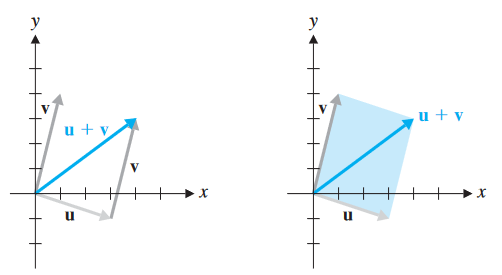
\includegraphics[scale=0.7]{example1-1-1.png}
\end{center}

\subsection*{Scalar Multiplication}
$$c\*{v}=c[\*{v}_1,\*{v}_2]=[c\*{v}_1, c\*{v}_2]$$

\subsection*{Example}
If $\*{v} = [2,-4]$, compute and draw $2\*{v}$, $\frac{1}{2}\*{v}$, and $-2\*{v}$

\subsection*{Solution}
\begin{enumerate}
    \item[] $2\*{v} = [2(-2),2(4)] = [-4,8]$
    \item[] $\frac{1}{2}\*{v} = [\frac{1}{2}(-2),\frac{1}{2}(4)] = [1,-2]$
    \item[] $-2\*{v} = [-2(-2),-2(4)] = [4,-8]$
\end{enumerate}
\begin{center}
    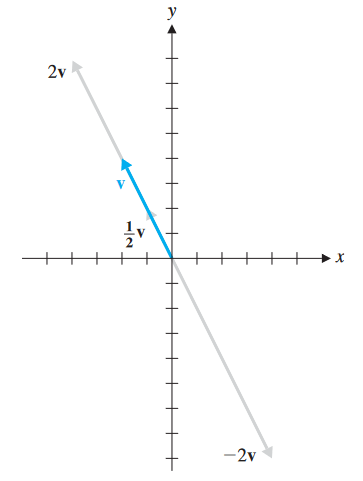
\includegraphics[scale=0.5]{example1-2-1.png}
\end{center}

\subsection*{Algebraic Properties of Vectors in $\mathbb{R}^n$}
Let \textbf{u}, \textbf{v}, and \textbf{w} be vectors in $\mathbb{R}^n$ and let
$c$ and $d$ be scalars. Then
\begin{enumerate}[(a)]
    \item $\*{u+v=v+u}$
    \item $\*{(u + v) + w = u + (v + w)}$
    \item $\*{u + 0 = u}$
    \item $\*{u + (-u) = 0}$
    \item $c\*{(u + v)=}c\*{u}+c\*{v}$
    \item $(c+d)\*{u}=c\*{u}+d\*{u}$
    \item $c(d\*{u})=(cd)\*{u}$
    \item $1\*{u}=\*{u}$
\end{enumerate}

A vector $\*{v}$ is a \textbf{linear combination} of vectors $\*{v_1,v_2,\dots,v_k}$ if
there are scalars $c_1,c_2, \dots , c_k$ such that $\*{v}=c_1\*{v}_1,c_2\*{v}_2,\dots,c_k\*{v}_k$.
The scalars $c_1,c_2,\dots,c_k$ are called the coefficients of the linear combination.

\section{Length and Angle: The Dot Product}

\subsection*{The Dot Product}
If
$$\vec{u}=\begin{bmatrix}
        u_1 \\ u_2 \\ \dots \\ u_n
    \end{bmatrix} \quad \text{and} \quad
    \vec{v}=\begin{bmatrix}
        v_1 \\ v_2 \\ \dots \\ v_n
    \end{bmatrix}$$
then the dot product of $\*{u \cdot v} = u_1v_1 + u_2v_2 + \dots + u_nv_n$

\subsection*{Example}
Compute $\*{u \cdot v}$ when
$$\vec{u}=\begin{bmatrix}
        1 \\ 2 \\ -3
    \end{bmatrix} \quad \text{and} \quad
    \vec{v}=\begin{bmatrix}
        -3 \\ 5 \\ 2
    \end{bmatrix}$$

\subsection*{Solution}
$$\*{u \cdot v} = 1 \cdot (-3) + 2 \cdot 5 + (-3) \cdot 2 = 1$$

\subsection*{Theorem}
Let \textbf{u}, \textbf{v}, and \textbf{w} be vectors in $\mathbb{R}^n$ and let $c$
be a scalar. Then
\begin{enumerate}[(a)]
    \item $\*{u\cdot v=v\cdot u}$
    \item $\*{(u\cdot v)\cdot w=u\cdot(v\cdot w)}$
    \item $(c\*u)\cdot\*v=c(\*{u\cdot v})$
    \item $\*{u\cdot u}\geq 0$ and $\*{u\cdot u}=0$ if and only if $\*u=0$
\end{enumerate}

The \textbf{length} (or \textbf{norm}) of a vector \textbf{v} in $\mathbb{R}^n$ is the
nonnegative scalar $\Vert\*v\Vert$ defined by
$$\Vert\vec{v}\Vert=\sqrt{\vec{v}\cdot\vec{v}}=\sqrt{v_1^2+v_2^2+\dots+v_n^2}$$

\subsection*{Theorem}
Let \textbf{v} be a vector in $\mathbb{R}^n$ and let $c$ be a scalar. Then
\begin{enumerate}[(a)]
    \item $\Vert\*v\Vert=0$ if and only if $\*v=0$
    \item $\Vert c\*v\Vert=|c|\Vert\*v\Vert$
\end{enumerate}

\subsection*{Cauchy-Schwarz Inequality}
For all vectors \textbf{u} and \textbf{v} in $\mathbb{R}^n$,
$$\Vert\*{u\cdot v}\Vert\leq\Vert\*u\Vert \Vert\*v\Vert$$

\subsection*{The Triangle Inequality}
For all vectors \textbf{u} and \textbf{v} in $\mathbb{R}^n$,
$$\Vert\*{u+v}\Vert\leq\Vert\*u\Vert+\Vert\*v\Vert$$

\subsection*{Proof}
\begin{enumerate}
    \item[] $\Vert\*{u+v}\Vert^2=\*{(u+v)\cdot(u+v)}$
    \item[] $=\*{u\cdot u}+2(\*{u\cdot v})+\*{v\cdot v}$
    \item[] $\leq\Vert\*u\Vert^2+2|\*{u\cdot v}|+\Vert\*v\Vert^2$
    \item[] $\leq\Vert\*u\Vert^2+2\Vert\*u\Vert \Vert\*v\Vert+\Vert\*v\Vert^2$
    \item[] $=(\Vert\*u\Vert+\Vert\*v\Vert)^2$
\end{enumerate}

For nonzero vectors \textbf{u} and \textbf{v} in $\mathbb{R}^n$,
$$\cos{\theta}=\frac{\vec{u}\cdot\vec{v}}{\Vert\vec{u}\Vert \Vert\vec{v}\Vert}$$

Two vectors \textbf{u} and \textbf{v} are \textbf{orthogonal} to each other if
$\*{u\cdot v} = 0$

If \textbf{u} and \textbf{v} are vectors in $\mathbb{R}^n$ and $u\neq 0$, then the
\textbf{projection of v onto u} is the vector $\text{proj}_u(\*v)$ defined by
$$\text{proj}_u(\vec{v})=\frac{(\vec{u}\cdot\vec{v})}{\vec{u}\cdot\vec{u}}\vec{u}$$

\subsection*{Example}
Find the projection of \textbf{v} onto \textbf{u} in each case
\begin{enumerate}[(a)]
    \item $\vec{v}=\begin{bmatrix}
                  -1 \\ 3
              \end{bmatrix}$ and $\vec{u}=\begin{bmatrix}
                  2 \\ 1
              \end{bmatrix}$
    \item $\vec{v}=\begin{bmatrix}
                  1 \\ 2 \\ 3
              \end{bmatrix}$ and $\vec{u}=e_3$
    \item $\vec{v}=\begin{bmatrix}
                  1 \\ 2 \\ 3
              \end{bmatrix}$ and $\vec{u}=\begin{bmatrix}
                  1/2 \\ 1/2 \\ 1/\sqrt{2}
              \end{bmatrix}$
\end{enumerate}

\subsection*{Solution}
\begin{enumerate}[(a)]
    \item $\*{u\cdot v}=1$ and $\*{u\cdot u}=5$ so
          $$\text{proj}_u(v)=\left(\frac{u\cdot v}{u\cdot u}\right)u=\frac{1}{5}\begin{bmatrix}
                  2 \\ 1
              \end{bmatrix}=\begin{bmatrix}
                  2/5 \\ 1/5
              \end{bmatrix}$$
    \item Since $\*e_3$ is a unit vector,
          $$\text{proj}_{e_3}(v)=(e_3\cdot v)e_3=\begin{bmatrix}
                  0 \\ 0 \\ 3
              \end{bmatrix}$$
    \item We see that $\Vert\*u\Vert=1$. Thus,
          $$\text{proj}_u(v)=(u\cdot v)u=\frac{3(1+\sqrt{2})}{4}\begin{bmatrix}
                  1 \\ 1 \\ \sqrt{2}
              \end{bmatrix}$$
\end{enumerate}

\section{Lines and Planes}
The vector \textbf{n} is perpendicular to the line - that is, it is
\textbf{orthogonal} to any vector \textbf{x} that is parallel to the line – and it
is called a \textbf{normal vector} to the line. The equation $\*{n\cdot x} = 0$ is
the \textbf{normal form} of the equation of $l$.
\begin{center}
    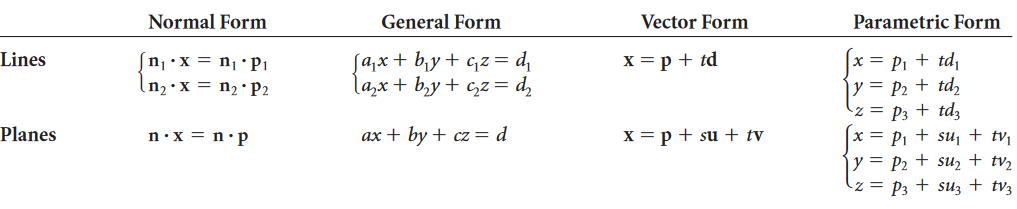
\includegraphics[scale=0.55]{example1-3-1.png}
\end{center}
\begin{enumerate}
    \item[] $d(B,l)=\cfrac{ax_0+by_0-c}{\sqrt{a^2+b^2}}$
    \item[] $d(B,P)=\cfrac{ax_0+by_0+cz_0-d}{\sqrt{a^2+b^2+c^2}}$
\end{enumerate}

\section{Code Vectors and Module Arithmetic}

\subsection*{Example}
Let $\*{u} = [1,1,0,1,0]$ and $\*{v} = [0,1,1,1,0]$ be two binary vectors of
length 5. Find $\*{u\cdot v}$.

\subsection*{Solution}
The calculation of $\*{u\cdot v}$ takes place in , so we have
$$\*{u\cdot v}=1\cdot0+1\cdot1+0\cdot1+1\cdot1+\mathbb{Z}_2 0\cdot0=0+1+0+1+0=0$$
\chapter{Systems of Linear Equations}

\section{Introduction to Systems of Linear Equations}
A linear equation in the n variables $x_1, x_2, \dots , x_n$ is an equation
that can be written in the form
$$a_1x_1+a_2x_2+\dots+a_nx_n=b$$
Where the coefficients $a_1, a_2, \dots , a_n$ and the constant term $b$ are constants.

\subsection*{Example}
Solve the system
\begin{enumerate}
    \item[] $x-y-z=2$
    \item[] $y+3z=5$
    \item[] $5z=10$
\end{enumerate}

\subsection*{Solution}
Starting from the last equation and working backward, we find successively that
$z=2$, $y=5-3(2)=-1$, and $x=2+(-1)+2=3$. So the unique solution is $[3,-1,2]$.

\section{Direct Methods for Solving Linear Systems}
The \textbf{coefficient matrix} contains the coefficients of the variables, and
the \textbf{augmented matrix} is the coefficient matrix augmented by an extra column
containing the constant terms.

A matrix is in \textbf{row echelon form} if it satisfies the following properties:
\begin{enumerate}
    \item Any rows consisting entirely of zeros are at the bottom
    \item In each nonzero row, the first nonzero entry (called the leading entry)
          is in a column to the left of any leading entries below it
\end{enumerate}

\subsection*{Example}
Reduce the following matrix to echelon form:
$$\begin{bmatrix}
        1  & 2 & -4 & -4 & 5 \\
        2  & 4 & 0  & 0  & 2 \\
        2  & 3 & 2  & 1  & 5 \\
        -1 & 1 & 3  & 6  & 5
    \end{bmatrix}$$

\subsection*{Solution}

\begin{enumerate}
    \item[] $\begin{bmatrix}
                  1  & 2 & -4 & -4 & 5 \\
                  2  & 4 & 0  & 0  & 2 \\
                  2  & 3 & 2  & 1  & 5 \\
                  -1 & 1 & 3  & 6  & 5
              \end{bmatrix}
              \arrows3{R_2-2R_1}{R_3-2R_1}{R_4+R_1}
              \begin{bmatrix}
                  1 & 2  & -4 & -4 & 5  \\
                  0 & 0  & 8  & 8  & -8 \\
                  0 & -1 & 10 & 0  & -5 \\
                  0 & 3  & -1 & 2  & 10
              \end{bmatrix}$
    \item[] $\arrows1{R_2 \leftrightarrow R_3}
              \begin{bmatrix}
                  1 & 2  & -4 & -4 & 5  \\
                  0 & -1 & 10 & 9  & -5 \\
                  0 & 0  & 8  & 8  & -8 \\
                  0 & 3  & -1 & 2  & 10
              \end{bmatrix}$
    \item[] $\arrows1{R_4+3R_2}
              \begin{bmatrix}
                  1 & 2  & -4 & -4 & 5  \\
                  0 & -1 & 10 & 9  & -5 \\
                  0 & 0  & 8  & 8  & -8 \\
                  0 & 0  & 29 & 29 & 5
              \end{bmatrix}$
    \item[] $\arrows1{\frac{1}{8}R_3}
              \begin{bmatrix}
                  1 & 2  & -4 & -4 & 5  \\
                  0 & -1 & 10 & 9  & -5 \\
                  0 & 0  & 1  & 1  & -1 \\
                  0 & 3  & -1 & 2  & 10
              \end{bmatrix}$
    \item[] $\arrows1{R_4-29R_3}
              \begin{bmatrix}
                  1 & 2  & -4 & -4 & 5  \\
                  0 & -1 & 10 & 9  & -5 \\
                  0 & 0  & 1  & 1  & -1 \\
                  0 & 0  & 0  & 0  & 24
              \end{bmatrix}$
\end{enumerate}

\subsection*{Gaussian Elimination}
When row reduction is applied to the augmented matrix of a system of linear
equations, we create an equivalent system that can be solved by back substitution.
\begin{enumerate}
    \item Write the augmented matrix of the system of linear equations.
    \item Use elementary row operations to reduce the augmented matrix to row echelon form.
    \item Using back substitution, solve the equivalent system that corresponds to the row-reduced matrix.
\end{enumerate}

The \textbf{rank} of a matrix is the number of nonzero rows in its row echelon form.

\subsection*{Example}
Solve the system:
\begin{enumerate}
    \item[] $x_1-x_2+2x_3=3$
    \item[] $x_1+2x_2-x_3=-3$
    \item[] $2x_2-2x_3=1$
\end{enumerate}

\subsection*{Solution}
\begin{enumerate}
    \item[] $\begin{bmatrix}
                  1 & -1 & 2  & 3  \\
                  1 & 2  & -1 & -3 \\
                  0 & 2  & 2  & 1
              \end{bmatrix} \arrows1{R_2-R_1} \begin{bmatrix}
                  1 & -1 & 2  & 3  \\
                  0 & 3  & -3 & 6  \\
                  0 & 2  & -2 & -1
              \end{bmatrix}$
    \item[] $\arrows1{\frac{1}{3}R_2}\begin{bmatrix}
                  1 & -1 & 2  & 3  \\
                  0 & 1  & -1 & -2 \\
                  0 & 2  & -2 & 1
              \end{bmatrix}\arrows1{R_3-2R_2}\begin{bmatrix}
                  1 & -1 & 2  & 3  \\
                  0 & 1  & -1 & -2 \\
                  0 & 0  & 0  & 5
              \end{bmatrix}$
\end{enumerate}
Leading to the impossible equation $0=5$. Thus, the system has no solutions.

\subsection*{Gauss-Jordan Elimination}
Modification of Gaussian elimination greatly simplifies the back substitution phase
and is particularly helpful when calculations are being done by hand or on a system
with infinitely many solutions. This method relies on reducing the augmented matrix even further.
\begin{enumerate}
    \item Write the augmented matrix of the system of linear equations.
    \item Use elementary row operations to reduce the augmented matrix to row echelon form.
    \item If the resulting system is consistent, solve for the leading variables in terms of any remaining free variables.
\end{enumerate}

A matrix is in \textbf{reduced row echelon form} if it satisfies the following properties:
\begin{enumerate}
    \item It is in row echelon form.
    \item The leading entry in each nonzero row is a 1 (called a leading 1).
    \item Each column containing a leading 1 has zeroes everywhere else.
\end{enumerate}

\subsection*{Example}
Determine whether the lines $\*x=\*p+s\*u$ and $\*x=\*q+t\*v$ intersect and,
if so find their point of intersection when
$$\*p=\begin{bmatrix}
        1 \\ 0 \\ -1
    \end{bmatrix} \quad \*q=\begin{bmatrix}
        0 \\ 2 \\ 1
    \end{bmatrix} \quad \*u=\begin{bmatrix}
        1 \\1\\1
    \end{bmatrix} \quad \*v=\begin{bmatrix}
        3 \\ -1 \\ -1
    \end{bmatrix}$$

\subsection*{Solution}
$$\*x=\*p+s\*u=\*q+t\*v \quad\text{or}\quad s\*u-t\*v=\*q-\*p$$
\begin{enumerate}
    \item[] $s-3t=-1$
    \item[] $s+t=2$
    \item[] $s+t=2$
\end{enumerate}
From this, we find that $s=\frac{5}{4}$, $t=\frac{3}{4}$.

The point of intersection is therefore
$$\begin{bmatrix}
        x \\ y\\ z
    \end{bmatrix}=\begin{bmatrix}
        1 \\ 0 \\ -1
    \end{bmatrix}+\frac{5}{4}\begin{bmatrix}
        1 \\ 1\\ 1
    \end{bmatrix}=\begin{bmatrix}
        9/4 \\ 5/4 \\ 1/4
    \end{bmatrix}$$

A system of linear equations is called \textbf{homogeneous} if the
constant term in each equation is zero.

\section{Spanning Sets and Linear Independence}

\subsection*{Example}
Is the vector $\begin{bmatrix}
        1 \\ 2 \\ 3
    \end{bmatrix}$ a linear combination of the vectors $\begin{bmatrix}
        1 \\ 0 \\ 3
    \end{bmatrix}$ and $\begin{bmatrix}
        -1 \\ 1 \\ -3
    \end{bmatrix}$?

\subsection*{Solution}
We want to find scalars $x$ and $y$ such that
$$x\begin{bmatrix}
        1 \\ 0 \\ 3
    \end{bmatrix}+y\begin{bmatrix}
        -1 \\ 1 \\ -3
    \end{bmatrix}=\begin{bmatrix}
        1 \\ 2 \\ 3
    \end{bmatrix}$$

Expanding, we obtain the system
\begin{enumerate}
    \item[] $x-y=1$
    \item[] $y=2$
    \item[] $3x-3y=3$
\end{enumerate}

Whose augmented matrix is
$$\begin{bmatrix}
        1 & -1 & 1 \\
        0 & 1  & 2 \\
        3 & -3 & 3
    \end{bmatrix}\arrows1{ref}\begin{bmatrix}
        1 & 0 & 3 \\
        0 & 1 & 2 \\
        0 & 0 & 0
    \end{bmatrix}$$

So the solution is $x=3$, $y=2$, and the corresponding linear combination is
$$3\begin{bmatrix}
        1 \\ 0 \\ 3
    \end{bmatrix}+2\begin{bmatrix}
        -1 \\ 1 \\ 3
    \end{bmatrix}=\begin{bmatrix}
        1 \\ 2 \\ 3
    \end{bmatrix}$$

If $S=\{\*v_1,\*v_2,\dots,\*v_k\}$  is a set of vectors in $\mathbb{R}^n$, then
the set of all linear combinations of $\*v_1,\*v_2,\dots,\*v_k$ is called
the \textbf{}{span} of $\*v_1,\*v_2,\dots,\*v_k$ and is denoted by span($\*v_1,\*v_2,\dots,\*v_k$)
or span($S$). If span($S$) = $\mathbb{R}^n$, then $S$ is called a
\textbf{spanning set} for $\mathbb{R}^n$.

\subsection*{Example}
Show that
$$\mathbb{R}^2=\text{span}\left(\begin{bmatrix}
            2 \\ -1
        \end{bmatrix},\begin{bmatrix}
            1 \\ 3
        \end{bmatrix}\right)$$

\subsection*{Solution}
We need to show that an arbitrary vector $\begin{bmatrix}
        a \\ b
    \end{bmatrix}$ can be written as a linear combination of $\begin{bmatrix}
        2 \\ -1
    \end{bmatrix}$ and $\begin{bmatrix}
        1 \\ 3
    \end{bmatrix}$.

Using the augmented matrix and row reduction we produce:
$$\begin{bmatrix}
        2  & 1 & a \\
        -1 & 3 & b
    \end{bmatrix}\arrows1{R_1\leftrightarrow R_2}\begin{bmatrix}
        -1 & 3 & b \\
        2  & 1 & a
    \end{bmatrix}\arrows1{R_2+2R_1}\begin{bmatrix}
        -1 & 0 & b    \\
        0  & 7 & a+2b
    \end{bmatrix}$$
$$\arrows1{\frac{1}{7}R_2}\begin{bmatrix}
        -1 & 3 & b        \\
        0  & 1 & (a+2b)/7
    \end{bmatrix}\arrows1{R_1-3R_2}\begin{bmatrix}
        -1 & 0 & (b-3a)/7 \\
        0  & 1 & (a+2b)/7
    \end{bmatrix}$$
$$x=\frac{3a-b}{7} \qquad \text{and} \qquad y=\frac{(a+2b)}{7}$$
Thus,
$$\frac{3a-b}{7}\begin{bmatrix}
        2 \\ -1
    \end{bmatrix}+\frac{a+2b}{7}\begin{bmatrix}
        1 \\ 3
    \end{bmatrix}=\begin{bmatrix}
        a \\ b
    \end{bmatrix}$$

A set of vectors $\*v_1,\*v_2,\dots,\*v_k$ is \textbf{linearly dependent} if there
are scalars $c_1,c_2,\dots,c_k$, at least one of which is not zero, such that
$$c_1\*v_1+c_2\*v_2+\dots+c_k\*v_k=0$$
A set of vectors that is not linearly dependent is called \textbf{linearly independent}.

\subsection*{Example}
Determine whether the following set of vectors are linearly independent:
$$\begin{bmatrix}
        1 \\ 2 \\ 0
    \end{bmatrix},\begin{bmatrix}
        1 \\ 1 \\ -1
    \end{bmatrix},\begin{bmatrix}
        1 \\ 4 \\ 2
    \end{bmatrix}$$

\subsection*{Solution}
\[
    \begin{bmatrix}
        1 & 1  & 1 & 0 \\
        2 & 1  & 4 & 0 \\
        0 & -1 & 2 & 0
    \end{bmatrix}\arrows1{R_2-2R_1}\begin{bmatrix}
        1 & 1  & 1 & 0 \\
        0 & -1 & 2 & 0 \\
        0 & -1 & 2 & 0
    \end{bmatrix}\arrows3{R_1+R_2}{R_3-R_2}{-R_2}\begin{bmatrix}
        1 & 0 & 3  & 0 \\
        0 & 1 & -2 & 0 \\
        0 & 0 & 0  & 0
    \end{bmatrix}
\]

\begin{enumerate}
    \item[] $c_1+3c_3=0 \qquad c_2-2c_3=0$
    \item[] $c_1=-3c_3 \qquad c_2=2c_3$
\end{enumerate}

\[
    -3c_3\begin{bmatrix}
        1 \\ 2 \\ 0
    \end{bmatrix}+2c_3\begin{bmatrix}
        1 \\ 1 \\ -1
    \end{bmatrix}+c_3\begin{bmatrix}
        1 \\ 4 \\ 2
    \end{bmatrix}=\begin{bmatrix}
        0 \\ 0 \\ 0
    \end{bmatrix}
\]

\section{Applications}

\subsection*{Example}
The combustion of ammonia ($\text{NH}_3$) in oxygen produces nitrogen
($\text{N}_2$) and water. Find a balanced chemical equation for this reaction.

\subsection*{Solution}
\[w{NH}_3+xO_2\to yN_2+zH_2O\]
\begin{enumerate}
    \item[] Nitrogen: $w=2y$
    \item[] Hydrogen: $3w=2z$
    \item[] Oxygen: $2x=z$
\end{enumerate}
\[
    \begin{matrix}
        w-2y=0  \\
        3w-2z=0 \\
        2x-z=0
    \end{matrix}\to\begin{bmatrix}
        1 & 0 & -2 & 0  & 0   \\
        3 & 0 & 0  & -2 & 0 & \\
        0 & 2 & 0  & -1 & 0
    \end{bmatrix}\arrows1{rref}\begin{bmatrix}
        1 & 0 & 0 & -2/3 & 0 \\
        0 & 1 & 0 & -1/2 & 0 \\
        0 & 0 & 1 & -1/3 & 0
    \end{bmatrix}
\]

\begin{align*}
    w=\frac{2}{3}z \qquad x=\frac{1}{2}z \qquad y=\frac{1}{3}z \\
    w=4 \qquad x=3 \qquad y=2 \qquad z=6                       \\
    4{NH}_3+3O_2\to2N_2+6H_2O
\end{align*}
\chapter{Matrices}

\section{Matrix Operations}

\subsection*{Matrix Addition and Scalar Multiplication}
The \textbf{sum} of matrix A and B is obtained by adding the corresponding entries.
\[A+B=[a_{ij}+b_{ij}]\]

\subsection*{Example}
Let
\[
    A=\begin{bmatrix}
        1  & 4 & 0 \\
        -2 & 6 & 5
    \end{bmatrix} \qquad B=\begin{bmatrix}
        -3 & 1 & -1 \\
        3  & 0 & 2
    \end{bmatrix} \qquad C=\begin{bmatrix}
        4 & 3 \\
        2 & 1
    \end{bmatrix}
\]
Then
\[A+B=\begin{bmatrix}
        -2 & 5 & -1 \\
        1  & 6 & 7
    \end{bmatrix}\]
but neither $A+C$ not $B+C$ is defined.

The \textbf{scalar multiple} $cA$ is the matrix obtained by multiplying each
entry of $A$ by $c$.
\[cA=c[a_{ij}]=[ca_{ij}]\]

\subsection*{Example}
\[
    2A=\begin{bmatrix}
        2  & 8  & 0  \\
        -4 & 12 & 10
    \end{bmatrix} \qquad
    \frac{1}{2}A=\begin{bmatrix}
        1/2 & 2 & 0   \\
        -1  & 3 & 5/2
    \end{bmatrix} \qquad
    (-1)A=\begin{bmatrix}
        -1 & -4 & 0  \\
        2  & -6 & -5
    \end{bmatrix}
\]

\subsection*{Matrix Multiplication}
If $A$ is an $m\times n$ matrix and $B$ is an $n\times r$ matrix, then the \textbf{product}
$C=AB$ is an $m\times r$ matrix. The $(i,j)$ entry of the product is computed as follows:
\[c_{ij}=a_{i1}b_{1j}+a_{i2}b_{2j}+\dots+a_{in}b_{nj}\]
or
\[c_{ij}=\sum_{k=1}^n a_{ik}b_{kj}\]

\subsection*{Example}
Compute $AB$ if
\[
    A=\begin{bmatrix}
        1  & 3  & -1 \\
        -2 & -1 & 1
    \end{bmatrix} \quad \text{and} \quad
    B=\begin{bmatrix}
        -4 & 0  & 3  & -1 \\
        5  & -2 & -1 & 1  \\
        -1 & 2  & 0  & 6
    \end{bmatrix}
\]

\subsection*{Solution}
Since $A$ is $2\times$ and $B$ is $3\times$, $AB$ will be a $2\times4$ matrix.
\begin{align*}
    c_{11} & =1(-4)+3(5)+(-1)(-1)=12     \\
    c_{12} & =1(0)+3(-2)+(-1)(2)=-8      \\
    c_{13} & =1(3)+3(-1)+(-1)(0)=0       \\
    c_{14} & =1(-1)+3(1)+(-1)(6)=-4      \\
    c_{21} & =(-2)(-4)+(-1)(5)+(1)(-1)=2 \\
    c_{22} & =(-2)(0)+(-1)(-2)+(1)(2)=4  \\
    c_{23} & =(-2)(3)+(-1)(-1)+(1)(0)=-5 \\
    c_{24} & =(-2)(-1)+(-1)(1)+(1)(6)=7
\end{align*}
Thus, product matrix is given by
\[AB=\begin{bmatrix}
        12 & -8 & 0  & -4 \\
        2  & 4  & -5 & 7
    \end{bmatrix}\]

\subsection*{Matrix Powers}
\[A^k=AA\dots A\]
If $A$ is a square matrix and $r$ and $s$ are nonnegative integers, then
\begin{enumerate}
    \item $A^rA^s=A^{r+s}$
    \item $(A^r)^s=A^{rs}$
\end{enumerate}

\subsection*{Transpose of a Matrix}
The \textbf{transpose} of an $m\times n$ matrix $A$ is the $n\times m$ matrix $A^T$
obtained by interchanging the rows and columns of $A$. That is, the $i$the column of
$A^T$ is the $i$th row of $A$ for all $i$.

\subsection*{Example}
Let
\[
    A=\begin{bmatrix}
        1 & 3 & 2 \\
        5 & 0 & 1
    \end{bmatrix} \qquad
    B=\begin{bmatrix}
        a & b \\
        c & d
    \end{bmatrix} \qquad
    C=\begin{bmatrix}
        5 & -1 & 2
    \end{bmatrix}
\]
Then their transposes are
\[
    A=\begin{bmatrix}
        1 & 5 \\
        3 & 0 \\
        2 & 1
    \end{bmatrix} \qquad
    B=\begin{bmatrix}
        a & c \\
        b & d
    \end{bmatrix} \qquad
    C=\begin{bmatrix}
        5 \\ -1 \\ 2
    \end{bmatrix}
\]

The dot product of two vectors \textbf{u} and \textbf{b} can be denoted by $\*u^T\*v$.
A square matrix is \textbf{symmetric} if $A^T=A$ (if $A$ is equal to its own transpose).

\section{Matrix Algebra}

\subsection*{Properties of Addition and Scalar Multiplication}
Let $A$, $B$, and $C$ be matrices of the same size and let $c$ and $d$ be scalars. Then
\begin{enumerate}[(a)]
    \item $A+B=B+A$
    \item $(A+B)+C=A+(B+C)$
    \item $A+0=A$
    \item $A+(-A)=0$
    \item $c(A+B)=cA+cB$
    \item $(c+d)A=cA+dA$
    \item $c(dA)=(cd)A$
    \item $1A=A$
\end{enumerate}

A linear combination of matrices looks like
\[c_1A_1+c_2A_2+\dots+c_kA_k\]
Where $c_1, c_2, \dots, c_k$ are the \textbf{coefficicents} of the linear combination.

\subsection*{Example}
Let $A_1=\begin{bmatrix}
        0  & 1 \\
        -1 & 0
    \end{bmatrix}$, $A_2=\begin{bmatrix}
        1 & 0 \\
        0 & 1
    \end{bmatrix}$, and $A_3=\begin{bmatrix}
        1 & 1 \\
        1 & 1
    \end{bmatrix}$. \\
Is $B=\begin{bmatrix}
        1 & 4 \\
        2 & 1
    \end{bmatrix}$ a linear combination of $A_1$, $A_2$, and $A_3$?

\subsection*{Solution}
We want to find scalars $c_1$, $c_2$, and $c_3$ such that $c_1A_1+c_2A_2+c_3A_3=B$. Thus,
\[
    c_1\begin{bmatrix}
        0  & 1 \\
        -1 & 0
    \end{bmatrix}+
    c_2\begin{bmatrix}
        1 & 0 \\
        0 & 1
    \end{bmatrix}+
    c_3\begin{bmatrix}
        1 & 1 \\
        1 & 1
    \end{bmatrix}=
    \begin{bmatrix}
        1 & 4 \\
        2 & 1
    \end{bmatrix}
\]
The left-hand side of this equation can be rewritten as
\[\begin{bmatrix}
        c_2+c_3  & c_1+c_3 \\
        -c_1+c_3 & c_2+c_3
    \end{bmatrix}\]
Comparing entries and using the definition of the matrix equality, we have four linear equations
\begin{align*}
    c_2+c_3  & =1 \\
    c_1+c_3  & =4 \\
    -c_1+c_3 & =2 \\
    c_2+c_3  & =1
\end{align*}
Gauss-Jordan elimination easily gives
\[
    \left[\begin{array}{ccc|c}
            0  & 1 & 1 & 1 \\
            1  & 0 & 1 & 4 \\
            -1 & 0 & 1 & 2 \\
            0  & 1 & 1 & 1
        \end{array}\right]\to
    \left[\begin{array}{ccc|c}
            1 & 0 & 0 & 1  \\
            0 & 1 & 0 & -2 \\
            0 & 0 & 1 & 3  \\
            0 & 0 & 0 & 0
        \end{array}\right]
\]
so $c_1=1$, $c_2=-2$, and $c_3=3$. Thus, $A_1-2A_2+3A_3=B$.

The \textbf{span} of a set of matrices is the set of all linear combinations of
the matrices.

\subsection*{Example}
Describe the span of the matrices $A_1$, $A_2$, and $A_3$ from the previous example.

\subsection*{Solution}
Write out a general linear combination of $A_1$, $A_2$, and $A_3$.
\begin{align*}
    c_1A_1+c_2A_2+c_3A_3 & =
    c_1\begin{bmatrix}
        0  & 1 \\
        -1 & 0
    \end{bmatrix}+
    c_2\begin{bmatrix}
        1 & 0 \\
        0 & 1
    \end{bmatrix}+
    c_3\begin{bmatrix}
        1 & 1 \\
        1 & 1
    \end{bmatrix}                      \\
                         & =\begin{bmatrix}
        c_2+c_3  & c_1+c_3 \\
        -c_1+c_3 & c_2+c_3
    \end{bmatrix}
\end{align*}
Suppose we want to know when the matrix $\begin{bmatrix}
        w & x \\
        y & z
    \end{bmatrix}$ is in span $(A_1,A_2,A_3)$. We know that it is when
\[
    \begin{bmatrix}
        c_2+c_3  & c_1+c_3 \\
        -c_1+c_3 & c_2+c_3
    \end{bmatrix}=
    \begin{bmatrix}
        w & x \\
        y & z
    \end{bmatrix}
\]
for some choice of scalars $c_1, c_2, c_3$. This gives a system of lienar equations
whose left-hand side is exactly the same as in the previous example but whose
right-hand side is general. The augmented matrix of this system is
\[\left[\begin{array}{ccc|c}
            0  & 1 & 1 & w \\
            1  & 0 & 1 & x \\
            -1 & 0 & 1 & y \\
            0  & 1 & 1 & z
        \end{array}\right]\]
and row reduction produces
\[
    \left[\begin{array}{ccc|c}
            0  & 1 & 1 & w \\
            1  & 0 & 1 & x \\
            -1 & 0 & 1 & y \\
            0  & 1 & 1 & z
        \end{array}\right]\to
    \left[\begin{array}{ccc|c}
            1 & 0 & 0 & \frac{1}{2}x-\frac{1}{2}y    \\
            0 & 1 & 0 & -\frac{1}{2}x-\frac{1}{2}y+w \\
            0 & 0 & 1 & \frac{1}{2}x+\frac{1}{2}y    \\
            0 & 0 & 0 & w-z
        \end{array}\right]
\]
The only restriction comes from the last row, where we must have $w-z=0$ to have a
solution. Thus, the span of $A_1$, $A_2$, and $A_3$ consists of all matrices
$\begin{bmatrix}
        w & x \\
        y & z
    \end{bmatrix}$ for which $w=z$. That is, span$(A_1,A_2,A_3)=\left\{\begin{bmatrix}
        w & x \\
        y & w
    \end{bmatrix}\right\}$

Matrices $A_1, A_2, \dots, A_k$ are \textbf{linearly independent} if the only solution of
\[c_1A_1+c_2A_2+\dots+c_kA_k=0\]
Is the trivial one: $c_1=c_2=\dots=c_k=0$. If not, the matrices are \textbf{linearly dependent}.

\subsection*{Properties of Matrix Multiplication}
Let $A$, $B$, and $C$ be matrices and let $k$ be a scalar. Then
\begin{enumerate}[(a)]
    \item $A(BC)=(AB)C$
    \item $A(B+C)=AB+AC$
    \item $(A+B)C=AC+BC$
    \item $k(AB)=(kA)B=A(kB)$
    \item $I_mA=A=AI_n$ if $A$ is $m\times n$
\end{enumerate}

\subsection*{Properties of Transpose}
Let $A$ and $B$ be matrices and let $k$ be a scalar. Then
\begin{enumerate}[(a)]
    \item $(A^T)^T=A$
    \item $(A+B)^T=A^T+B^T$
    \item $(kA)^T=k(A^T)$
    \item $(AB)^T=B^TA^T$
    \item $(A^r)^T=(A^T)^r$ for all nonnegative integers $r$
\end{enumerate}

\subsection*{Theorem}
\begin{enumerate}[(a)]
    \item If $A$ is a square matrix, then $A+A^T$ is a symmetric matrix.
    \item For any matrix $A$, $AA^T$, and $A^TA$ are symmetric matrices.
\end{enumerate}

\section{Inverse of a Matrix}

\subsection*{Definition}
If $A$ is an $n\times n$ matrix, an \textbf{inverse} of $A$ is an $n\times n$ matrix
$A'$ with the property that
\[AA'=I \qquad \text{and} \qquad A'A=I\]
where $I=I_n$ is the $n\times n$ identity matrix. If such an $A'$ exists, then $A$
is called \textbf{invertible.}

\subsection*{Example}
If $A=\begin{bmatrix}
        2 & 5 \\
        1 & 3
    \end{bmatrix}$, then $A'=\begin{bmatrix}
        3  & -5 \\
        -1 & 2
    \end{bmatrix}$ is an inverse of $A$, since\\ $AA'=\begin{bmatrix}
        2 & 5 \\
        1 & 3
    \end{bmatrix}\begin{bmatrix}
        3  & -5 \\
        -1 & 2
    \end{bmatrix}=\begin{bmatrix}
        1 & 0 \\
        0 & 1
    \end{bmatrix}$ and $A'A=\begin{bmatrix}
        3  & -5 \\
        -1 & 2
    \end{bmatrix}\begin{bmatrix}
        2 & 5 \\
        1 & 3
    \end{bmatrix}=\begin{bmatrix}
        1 & 0 \\
        0 & 1
    \end{bmatrix}$

\subsection*{Theorem}
If $A$ is an invertible matrix, then its inverse is unique.

\subsection*{Proof}
A standard way to show that there is just one of something is to show that there
cannot be more than one. So, suppose $A$ has two inverses, $A'$ and $A''$. Then
\[AA'=I=A'A \qquad \text{and} \qquad AA''=I=A''A\]
\[A'=A'I=A'(A'')=(A'A)A''=IA''=A''\]
Hence, $A'=A''$, and the inverse is unique.

\subsection*{Theorem}
If $A$ is an invertible $n\times n$ matrix, then the system of linear equations
given by $A\*x=\*b$ has the unique solution $\*x=A^{-1}\*b$ for any \textbf{b} in $\mathbb{R}^n$.

\subsection*{Theorem}
If $A=\begin{bmatrix}
        a & b \\
        c & d
    \end{bmatrix}$, then $A$ is invertible if $ad-bc\neq0$, in which case
\[A^{-1}=\frac{1}{ad-bc}\begin{bmatrix}
        d  & -b \\
        -c & a
    \end{bmatrix}\]
If $ad-bc=0$, then $A$ is not invertible.

The expression $ad-bc$ is called the \textbf{determinant} of $A$.

\subsection*{Example}
Find the inverses of $A=\begin{bmatrix}
        1 & 2 \\
        3 & 4
    \end{bmatrix}$ and $B=\begin{bmatrix}
        12 & -15 \\
        4  & -5
    \end{bmatrix}$, if they exist.

\subsection*{Solution}
We have det $A=1(4)-2(3)=-2\neq0$, so $A$ is invertible, with
\[A^{-1}=\frac{1}{-2}\begin{bmatrix}
        4  & -2 \\
        -3 & 1
    \end{bmatrix}=\begin{bmatrix}
        -2  & 1    \\
        3/2 & -1/2
    \end{bmatrix}\]
On the other hand, det $B=12(-5)-(-15)(4)=0$, so $B$ is not invertible.

\subsection*{Properties of Invertible Matrices}
\begin{enumerate}[(a)]
    \item If $A$ is an invertible matrix, then $A^{-1}$ is invertible and \[(A^{-1})^{-1}=A\]
    \item If $A$ is an invertible matrix and $c$ is a nonzero scalar, then $cA$ is an invertible matrix and \[(cA)^{-1}=\frac{1}{c}A^{-1}\]
    \item If $A$ and $B$ are invertible matrices of the same size, then $AB$ is invertible and \[(AB)^{-1}=B^{-1}A^{-1}\]
    \item If $A$ is an invertible matrix, then $A^T$ is invertible and \[(A^T)^{-1}=(A^{-1})^T\]
    \item If $A$ is an invertible matrix, then $A^n$ is invertible for all nonnegative integers $n$ and \[(A^n)^{-1}=(A^{-1})^n\]
\end{enumerate}

\subsection*{The Fundamental Theorem of Invertible Matrices}
Let $A$ be an $n\times n$ matrix. The following statements are equivalent:
\begin{enumerate}[(a)]
    \item $A$ is invertible.
    \item $A\*x=\*b$ has a unique solution for every $\*b$ in $\mathbb{R}^n$.
    \item $A\*x=0$ has only the trivial solution.
    \item The reduced row echelon form of $A$ is $I_n$.
    \item $A$ is a product of elementary matrices.
\end{enumerate}

\subsection*{Proof}
We will establish the theorem by proving the circular chain of implications
\[(a)\Rightarrow(b)\Rightarrow(c)\Rightarrow(d)\Rightarrow(e)\Rightarrow(a)\]
\begin{enumerate}
    \item[] $(a)\Rightarrow(b)$ We have already shown that if $A$ is invertible, then $A\*x-\*b$ has the unique solution $\*x=A^{-1}\*b$ for any \textbf{b} in $\mathbb{R}^n$.
    \item[] $(b)\Rightarrow(c)$ Assume that $A\*x-\*b$ has a unique solution for any $\*b$ in $\mathbb{R}^n$. This implies that $A\*x=0$ has a unique solution. But a homogeneous system $A\*x=0$ always has $\*x=0$ as one solution. So $\*x=0$ must be the solution.
    \item[] $(c)\Rightarrow(d)$ Suppose that $A\*x=0$ has only the trivial solution. The corresponding system of equations is
          \begin{align*}
              a_{11}x_1+a_{12}x_2+ & \dots+a_{1n}x_n=0 \\
              a_{21}x_1+a_{22}x_2+ & \dots+a_{2n}x_n=0 \\
                                   & \vdots            \\
              a_{n1}x_1+a_{n2}x_2+ & \dots+a_{nn}x_n=0
          \end{align*}
\end{enumerate}
and we are assuming that its solution is
\[x_1=0 \quad x_2=0 \quad \dots \quad x_n=0\]
In other words, Gauss-Jordan elimination applied to the augmented matrix of the system gives
\[
    [A|0]=
    \left[\begin{array}{cccc|c}
            a_{11} & a_{12} & \dots  & a_{1n} & 0      \\
            a_{21} & a_{22} & \dots  & a_{2n} & 0      \\
            \vdots & \vdots & \ddots & \vdots & \vdots \\
            a_{n1} & a_{n2} & \dots  & a_{nn} & 0
        \end{array}\right]\to
    \left[\begin{array}{cccc|c}
            1      & 0      & \dots  & 0      & 0      \\
            0      & 1      & \dots  & 0      & 0      \\
            \vdots & \vdots & \ddots & \vdots & \vdots \\
            0      & 0      & \dots  & 1      & 0
        \end{array}\right]=[I_n|0]
\]
Thus, the reduced row echelon form of $A$ is $I_n$.

\section{LU Factorization}

\subsection*{Definition}
Let $A$ be a square matrix. A factorization of $A$ as $A=LU$, where $L$ is unit
lower triangular and $U$ is upper triangular, is called \textbf{LU factorization} of $A$.

\subsection*{Example}
Row reduction of $A$ proceeds as follows:
\[
    A=\begin{bmatrix}
        2  & 1  & 3 \\
        4  & -1 & 3 \\
        -2 & 5  & 5
    \end{bmatrix}\arrows2{R_2-2R_1}{R_3+R_1}\begin{bmatrix}
        2 & 1  & 3  \\
        0 & -3 & -3 \\
        0 & 6  & 8
    \end{bmatrix}\arrows1{R_3+2R_2}\begin{bmatrix}
        2 & 1  & 3  \\
        0 & -3 & -3 \\
        0 & 0  & 2
    \end{bmatrix}=U
\]
The three elementary matrices $E_1, E_2, E_3$ that accomplish this reduction of $A$
to echelon form $U$ are
\[
    E_1=\begin{bmatrix}
        1  & 0 &   \\
        -2 & 1 & 0 \\
        0  & 0 & 1
    \end{bmatrix} \qquad E_2=\begin{bmatrix}
        1 & 0 & 0 \\
        0 & 1 & 0 \\
        1 & 0 & 1
    \end{bmatrix} \qquad E_3\begin{bmatrix}
        1 & 0 & 0 \\
        0 & 1 & 0 \\
        0 & 2 & 1
    \end{bmatrix}
\]
Hence,
\[E_3E_2E_1A=U\]
Solving for $A$, we get
\begin{align*}
    A=E_1^{-1}E_2^{-1}E_3^{-1}U & =\begin{bmatrix}
        1 & 0 & 0 \\
        2 & 1 & 0 \\
        0 & 0 & 1
    \end{bmatrix}\begin{bmatrix}
        1  & 0 & 0 \\
        0  & 1 & 0 \\
        -1 & 0 & 1
    \end{bmatrix}\begin{bmatrix}
        1 & 0  & 0 \\
        0 & 1  & 0 \\
        0 & -2 & 1
    \end{bmatrix}U \\
                                & =\begin{bmatrix}
        1  & 0  & 0 \\
        2  & 1  & 0 \\
        -1 & -2 & 1
    \end{bmatrix}U=LU
\end{align*}
Thus, $A$ can be factored as \[A=LU\]

The elementary row operations that were used are, in order:
\[
    \begin{aligned}[c]
         & R_2-2R_1             \\
         & R_3+R_1=R_3-(-1)R_1  \\
         & R_3+2R_2=R_3-(-2)R_2
    \end{aligned}
    \qquad
    \begin{aligned}[c]
         & \text{(multiplier = 2)}  \\
         & \text{(multiplier = -1)} \\
         & \text{(multiplier = -2)}
    \end{aligned}
\]
The multipliers are precisely the entries of $L$ that are below its diagonal.
\[L=\begin{bmatrix}
        1  & 0  & 0 \\
        2  & 1  & 0 \\
        -1 & -2 & 1
    \end{bmatrix}\]
and $L_{21}-2$, $L_{31}=-1$, and $L_{32}=-2$. Notice the elementary row operations
$R_i=kR_j$ has its multiplier $k$ placed in the $(i,j)$ entry of $L$.

\subsection*{$\*P^T\*{LU}$ Factorization}
This method is an adaptation of the LU factorization which handles row interchanges
during Gaussian elimination. $P$ is called the \textbf{permutation matrix}.

\subsection*{Theorem}
If $P$ is a permutation matrix, then $P^{-1}=P^T$.

\subsection*{Definition}
Let $A$ be a square matrix. A factorization of $A$ as $A=P^TLU$, where $P$ is a
permutation matrix, $L$ is unit lower triangular, and $U$ is upper triangular,
is called a $P^TLU$ factorization of $A$.

\subsection*{Example}
Find a $P^TLU$ factorization of $A=\begin{bmatrix}
        0 & 0 & 6 \\
        1 & 2 & 3 \\
        2 & 1 & 4
    \end{bmatrix}$.

\subsection*{Solution}
First we reduce $A$ to row echelon form.
\[
    A=\begin{bmatrix}
        0 & 0 & 6 \\
        1 & 2 & 3 \\
        2 & 1 & 4
    \end{bmatrix}\arrows1{R_1\leftrightarrow R_2}\begin{bmatrix}
        1 & 2 & 3 \\
        0 & 0 & 6 \\
        2 & 1 & 4
    \end{bmatrix}\arrows1{R_3-2R_1}\begin{bmatrix}
        1 & 2  & 3  \\
        0 & 0  & 6  \\
        0 & -3 & -2
    \end{bmatrix}
\]
\[\arrows1{R_2\leftrightarrow R_3}\begin{bmatrix}
        1 & 2  & 3  \\
        0 & -3 & -2 \\
        0 & 0  & 6
    \end{bmatrix}\]
We have used two row interchanges ($R_1\leftrightarrow R_2$ and then $R_2\leftrightarrow R_3$),
so the required permutation matrix is
\[
    P=P_2P_1=\begin{bmatrix}
        1 & 0 & 0 \\
        0 & 0 & 1 \\
        0 & 1 & 0
    \end{bmatrix}\begin{bmatrix}
        0 & 1 & 0 \\
        1 & 0 & 0 \\
        0 & 0 & 1
    \end{bmatrix}=\begin{bmatrix}
        0 & 1 & 0 \\
        0 & 0 & 1 \\
        1 & 0 & 0
    \end{bmatrix}
\]
We now find an $LU$ factorization of $PA$.
\[
    PA=\begin{bmatrix}
        0 & 1 & 0 \\
        0 & 0 & 1 \\
        1 & 0 & 0
    \end{bmatrix}\begin{bmatrix}
        0 & 0 & 6 \\
        1 & 2 & 3 \\
        2 & 1 & 4
    \end{bmatrix}=\begin{bmatrix}
        1 & 2 & 3 \\
        2 & 1 & 4 \\
        0 & 0 & 6
    \end{bmatrix}\arrows1{R_2-2R_1}\begin{bmatrix}
        1 & 2  & 3  \\
        0 & -3 & -2 \\
        0 & 0  & 6
    \end{bmatrix}=U
\]
Hence $L_{21}=2$, and so
\[
    A=P^TLU=\begin{bmatrix}
        0 & 0 & 1 \\
        1 & 0 & 0 \\
        0 & 1 & 0
    \end{bmatrix}\begin{bmatrix}
        1 & 0 & 0 \\
        2 & 1 & 0 \\
        0 & 0 & 1
    \end{bmatrix}\begin{bmatrix}
        1 & 2  & 3  \\
        0 & -3 & -2 \\
        0 & 0  & 6
    \end{bmatrix}
\]

\section{Subspaces, Basis, Dimension, and Rank}

\subsection*{Definition}
A \textbf{subspace} of $\mathbb{R}^n$ is any collection $S$ of vectors in
$\mathbb{R}^n$ such that
\begin{enumerate}[1.]
    \item The zero vector 0 is in $S$.
    \item If \textbf{u} and \textbf{v} are in $S$, then $\*{u+v}$ is in $S$.
    \item If \textbf{u} is in $S$ and $c$ is a scalar, then $c\*u$ is in $S$.
\end{enumerate}

\subsection*{Example}
Every line and place through the origin in $\mathbb{R}^3$ is a subspace of $\mathbb{R}^3$.
It should be clear geometrically that properties (1) through (3) are satisfied. Here
is an algebriac proof in the case of a plane through the origin. You are asked to give
the corresponding proof for a line.

Let $\mathscr{P}$ be a plane through the origin with direction vectors $\*v_1$ and
$\*v_2$. Hence, $\mathscr{P}=\text{span}(\*v_1,\*v_2)$. Ther zero vector 0 is in
$\mathscr{P}$, since $0=0\*v_1+0\*v_2$. Now let
\[\*u=c_1\*v_1+c_2\*v_2 \qquad \text{and} \qquad \*v=d_1\*v_1+d_2\*v_2\]
be two vectors in $\mathscr{P}$. Then
\[\*{u+v}=(c_1\*v_1+c_2\*v_2)+(d_1\*v_1+d_2\*v_2)=(c_1+d_1)\*v_1+(c_2+d_2)\*v_2\]
Thus, \textbf{u+v} is a linear combination of $\*v_1$ and $\*v_2$ and so is in $\mathscr{P}$.

Now let $c$ be a scalar. Then
\[c\*u=c(c_1\*v_1+c_2\*v_2)=(cc_1)\*v_1+(cc_2)\*v_2\]
which shows that $c\*u$ is also a linear combination of $*v_1$ and $*v_2$ and is
therefore in $\mathscr{P}$. We have shown that $\mathscr{P}$ satisfies properties
(1) through (3) and hence is a subspace of $\mathbb{R}^3$.

\subsection*{Theorem}
Let $v_1, v_2, \dots, v_k$ be vectors in $\mathbb{R}^n$. Then span$(v_1, v_2, \dots, v_k)$
is a subspace of $\mathbb{R}^n$.

\subsection*{Example}
Show that the set of all vectors $\begin{bmatrix}
        x \\y\\z
    \end{bmatrix}$ that satisfy the conditions $x=3y$ and $z=-2y$ forms a subspace of $\mathbb{R}^3$.

\subsection*{Solution}
Substituting the two conditions into $\begin{bmatrix}
        x \\y\\z
    \end{bmatrix}$ yields
\[
    \begin{bmatrix}
        3y \\y\\-2y
    \end{bmatrix}=y\begin{bmatrix}
        3 \\1\\-2
    \end{bmatrix}
\]
Since $y$ is arbitrary, the given set of vectors is span$\left(\begin{bmatrix}
            3 \\1\\-2
        \end{bmatrix}\right)$ and is thus a subspace of $\mathbb{R}^3$.

\subsection*{Subspaces Associated with Matrices}

\subsection*{Definition}
Let $A$ be an $m\times n$ matrix.
\begin{enumerate}
    \item The \textbf{row space} of $A$ is the subspace row($A$) of $\mathbb{R}^n$ spanned by the rows of $A$.
    \item The \textbf{column space} of $A$ is the subspace col($A$) of $\mathbb{R}^m$ spanned by the columns of $A$.
\end{enumerate}

\subsection*{Example}
Consider the matrix \[A=\begin{bmatrix}
        1 & -1 \\
        0 & 1  \\
        3 & -3
    \end{bmatrix}\]
\begin{enumerate}[(a)]
    \item Determine whether $\*b=\begin{bmatrix}
                  1 \\2\\3
              \end{bmatrix}$ is in the column space of $A$.
    \item Determine whether $\*w=\begin{bmatrix}
                  4 & 5
              \end{bmatrix}$ is in the row space of $A$.
    \item Describe row($A$) and col($A$).
\end{enumerate}

\subsection*{Solution}
\begin{enumerate}[(a)]
    \item \textbf{b} is a linear combination of the columns of $A$ if and only if the linear system $A\*x=\*b$ is consistent.
          We row reduce the augmented matrix as follows: \[\left[\begin{array}{cc|c}
                      1 & -1 & 1 \\
                      0 & 1  & 2 \\
                      3 & -3 & 3
                  \end{array}\right]\to \left[\begin{array}{cc|c}
                      1 & 0 & 3 \\
                      0 & 1 & 2 \\
                      0 & 0 & 0
                  \end{array}\right]\]
          Thus, the system is consistent. Therefore, \textbf{b} is in col($A$).
    \item Elementary row operations simply create linear combinations of the rows of a matrix.
          That is, they produce vectors only in the row space of the matrix. If the vector \textbf{w}
          is in row($A$), then \textbf{w} is a linear combination of the rows of $A$, so if we augmente
          $A$ by \textbf{w} as $\left[\frac{A}{\*w}\right]$, it will be possible to apply elementary row
          operations to this augmented matrix to reduce it to $\left[\frac{A'}{0}\right]$ using only
          elementary row operations of the form $R_i+kR_j$, where $i>j$

          In this example, we have
          \[
              \left[\frac{A}{\*w}\right]=\begin{bmatrix}
                  1 & -1 \\
                  0 & 1  \\
                  3 & -3 \\ \hline
                  4 & 5
              \end{bmatrix}\arrows2{R_3-3R_1}{R-4-4R_1}\begin{bmatrix}
                  1 & -1 \\
                  0 & 1  \\
                  0 & 0  \\ \hline
                  0 & 9
              \end{bmatrix}\arrows1{R_4-9R_2}\begin{bmatrix}
                  1 & -1 \\
                  0 & 1  \\
                  0 & 0  \\ \hline
                  0 & 0
              \end{bmatrix}
          \]
          Therefore, \textbf{w} is a linear combination of the rows of $A$, and thus \textbf{w} is in row($A$).
    \item It is easy to check that, for any vector $\*w=\begin{bmatrix}
                  x & y
              \end{bmatrix}$, the augmented matrix $\left[\frac{A}{\*w}\right]$ reduces two
          \[\begin{bmatrix}
                  1 & 0 \\
                  0 & 1 \\
                  0 & 0 \\ \hline
                  0 & 0
              \end{bmatrix}\]
          in a similar fashion. Therefore, every vector in $\mathbb{R}^2$ is in row($A$), and so $\text{row}(A)=\mathbb{R}^2$.
\end{enumerate}

\subsection*{Definition}
Let $A$ be an $m\times n$ matrix. The \textbf{null space} of $A$ is the subspace of
$\mathbb{R}^n$ consisting of solutions of the homogeneous linear system $A\*x=0$. It
is denoted by null($A$).

\subsection*{Basis}

\subsection*{Definition}
A \textbf{basis} for a subspace $S$ of $\mathbb{R}^n$ is a set of vectors in $A$ that
\begin{enumerate}
    \item spans $A$ and
    \item is linearly independent
\end{enumerate}

\subsection*{Example}
The standard unit vectors $\*e_1,\*e_2,\dots,\*e_n$ in $\mathbb{R}^n$ are linearly
independent and span $\mathbb{R}^n$. Therefore, they form a basis for $\mathbb{R}^n$,
called the \textbf{standard basis}.

Following is a summary of the most effective procedure to use to find bases for the
row space, the column space, and the null space of a matrix $A$.

\begin{enumerate}
    \item Find the reduced row echelon form $R$ of $A$.
    \item Use the nonzero row vectors of $R$ to form a basis for row($A$).
    \item Use the column vectors of $A$ that correspond to the columns of $R$
          containing leading 1s to form a basis for col($A$).
    \item Solve for the leading variables of $R\*x=0$ in terms of the free variables,
          set the free variables equal to the parameters, substitute back into \textbf{x},
          and write the result as a linera combination of $f$ vectors. These $f$ vectors form a basis for null($A$).
\end{enumerate}

\subsection*{Dimension and Rank}

\subsection*{The Basis Theorem}
Let $S$ be a subspace of $\mathbb{R}^n$. Then any two bases for $S$ have the same
number of vectors.

\subsection*{Definition}
If $S$ is a subspace of $\mathbb{R}^n$, then the number of vectors in a basis for $S$
is called the \textbf{dimension} of $S$, denoted by dim $S$.

\subsection*{Example}
Since the standard basis for $\mathbb{R}^n$ has $n$ vectors, dim $\mathbb{R}^n=n$.

\subsection*{Definition}
The \textbf{rank} of a matrix $A$ is the dimension of its row and column spaces
and is denoted by rank($A$).

\subsection*{Definition}
The \textbf{nullity} of a matrix $A$ is the dimension of its null space and is denoted
by nullity($A$).

\subsection*{The Rank Theorem}
If $A$ is an $m\times n$ matrix, then
\[\text{rank}(A)+\text{nullity}(A)=n\]

\subsection*{Proof}
Let $R$ be the reduced row echelon form of $A$, and suppose that rank($A$)=$r$.
Then $R$ has $r$ leading 1s, so there are $r$ leading variables and $n-r$ free
variables in the solution to $A\*x=0$. Since dim(null($A$))=$n-r$, we have
\[\text{rank}(A)+\text{nullity}(A)=r+(n-r)=n\]

\subsection*{The Fundamental Theorem of Invertible Matrices}
Let $A$ be an $n\times n$ matrix. THe following statements are equivalent:
\begin{enumerate}[(a)]
    \item $A$ is invertible.
    \item $A\*x=\*b$ has a unique solution for every \textbf{b} in $\mathbb{R}^n$.
    \item $A\*x=0$ has only the trivial solution.
    \item The reduced row echelon form of $A$ is $I_n$.
    \item $A$ is a product of elementary matrices.
    \item rank($A$)=$n$
    \item nullity($A$)=0
    \item The column vectors of $A$ are linearly independent.
    \item The column vectors of $A$ span $\mathbb{R}^n$.
    \item The column vectors of $A$ form a basis for $\mathbb{R}^n$.
    \item The row vectors of $A$ are linearly independent.
    \item The row vectors of $A$ span $\mathbb{R}^n$.
    \item The row vectors of $A$ form a basis for $\mathbb{R}^n$.
\end{enumerate}

\subsection*{Coordinates}

\subsection*{Definition}
Let $S$ be a subspace of $\mathbb{R}^n$ and let $\mathcal{B}=\left\{\*v_1,\*v_2,\dots,\*v_k\right\}$
be a basis for $S$. Let \textbf{v} be a vector in $S$, and write
$\*v=c_1\*v_1+c_2\*v_2+\dots+c_k\*v_k$. Then $c_1+c_2+\dots+c_k$ are called the
\textbf{coordinates of v with respect to $\mathcal{B}$}, and the column vector
\[
    [\*v]_{\mathcal{B}}\begin{bmatrix}
        c_1 \\c_2\\ \vdots\\c_k
    \end{bmatrix}
\]
is called the \textbf{coordinate vectors of v with respect to $\mathcal{B}$}.

\subsection*{Example}
Let $\mathcal{E}=\left\{\*e_1+\*e_2+\*e_3\right\}$ be the standard basis for
$\mathbb{R}^3$. Find the coordinate vector of \[\begin{bmatrix}
        2 \\7\\4
    \end{bmatrix}\] with respect to $\mathcal{E}$.

\subsection*{Solution}
Since $\*v=2\*e_1+7\*e_2+4\*e_3$, \[[\*v]_{\mathcal{E}}=\begin{bmatrix}
        2 \\7\\4
    \end{bmatrix}\]

\section{Intro to Linear Transformations}

\subsection*{Definition}
A transformation $T:\mathbb{R}^n\to\mathbb{R}^m$ is called a \textbf{linear transformation} if
\begin{enumerate}
    \item $T(\*u+\*v)=T(\*u)+T(\*v)$ for all \textbf{u} and \textbf{v} in $\mathbb{R}^n$ and
    \item $T(c\*v)=cT(\*v)$ for all \textbf{v} in $\mathbb{R}^n$ and all scalars $c$.
\end{enumerate}

\subsection*{Example}
Let $F:\mathbb{R}^2\to\mathbb{R}^2$ be the transformation that sends each point to its
reflection in the $x$-axis. Show that $F$ is a linear transformation.

\subsection*{Solution}
$F$ sends the point $(x,y)$ to the point $(x,-y)$. Thus, we write
\[
    F\begin{bmatrix}
        x \\y
    \end{bmatrix}=\begin{bmatrix}
        x \\-y
    \end{bmatrix}
\]
We could proceed to check that $F$ is linear, but it's faster to observe that
\[
    \begin{bmatrix}
        x \\-y
    \end{bmatrix}=x\begin{bmatrix}
        1 \\0
    \end{bmatrix}+y\begin{bmatrix}
        0 \\-1
    \end{bmatrix}=\begin{bmatrix}
        1 & 0  \\
        0 & -1
    \end{bmatrix}\begin{bmatrix}
        x \\y
    \end{bmatrix}
\]
Therefore, $F\begin{bmatrix}
        x \\y
    \end{bmatrix}=A\begin{bmatrix}
        x \\y
    \end{bmatrix}$, where $A=\begin{bmatrix}
        1 & 0  \\
        0 & -1
    \end{bmatrix}$, so $F$ is a matrix transformation. It now follows, that $F$ is a linear transformation.

\subsection*{Theorem}
Let $T:\mathbb{R}^m\to\mathbb{R}^n$ and $S:\mathbb{R}^n\to\mathbb{R}^p$ be linear transformations.
Then $S\circ T:\mathbb{R}^m\to\mathbb{R}^p$ is a linear transformation. Moreover, their
standard matrices are related by
\[
    [S\circ T]=[S][T]
\]

\subsection*{Inverse Transformations}

\subsection*{Definition}
Let $S$ and $S$ be linearl transformations form $\mathbb{R}^n$ to $\mathbb{R}^n$.
Then $S$ and $T$ are \textbf{inverse transformations} if $S\circ T=I_n$ and $T\circ S=I_n$.

\subsection*{Example}
Find the standard matrix of a $60^\circ$ clockwise rotation about the origin in $\mathbb{R}^n$.

\subsection*{Solution}
The matrix of a $60^\circ$ counterclockwise rotation about the origin is
\[
    [R_{60}]\begin{bmatrix}
        1/2        & -\sqrt{3}/2 \\
        \sqrt{3}/2 & 1/2
    \end{bmatrix}
\]
Since a $60^\circ$ clockwise rotation is the inverse of a $60^\circ$ counterclockwise rotation
\[
    [R_{-60}]=[(R_{60})^{-1}]=\begin{bmatrix}
        1/2        & -\sqrt{3}/2 \\
        \sqrt{3}/2 & 1/2
    \end{bmatrix}^{-1}=\begin{bmatrix}
        1/2         & \sqrt{3}/2 \\
        -\sqrt{3}/2 & 1/2
    \end{bmatrix}
\]
\chapter{Eigenvalues}

\section{Intro to Eigenvalues and Eigenvectors}

\subsection*{Definition}
Let $A$ be an $n\times n$ matrix. A scalar $\lambda$ is called an \textbf{eigenvalue}
of $A$ if there is a nonzero vector $\*x$ such that $A\*x=\lambda\*x$. Such a vector
$\*x$ is called an \textbf{eigenvector} of $A$ corresponding to $\lambda$.

\subsection*{Example}
Show that $\*x=\begin{bmatrix}
        1 \\1
    \end{bmatrix}$ is an eigenvector of $A=\begin{bmatrix}
        3 & 1 \\
        1 & 3
    \end{bmatrix}$ and find the corresponding eigenvalue.

\subsection*{Solution}
We compute
\[
    A\*x=\begin{bmatrix}
        3 & 1 \\
        1 & 3
    \end{bmatrix}\begin{bmatrix}
        1 \\1
    \end{bmatrix}=\begin{bmatrix}
        4 \\4
    \end{bmatrix}=4\begin{bmatrix}
        1 \\1
    \end{bmatrix}=4\*x
\]
from which it follows that $\*x$ is an eigenvector of $A$ corresponding to the eigenvalue 4.

\subsection*{Definition}
Let $A$ be an $n\times n$ matrix and let $\lambda$ be an eigenvalue of $A$. The collection
of all eigenvectors corresponding to $\lambda$, together with the zero vector, is called
the \textbf{eigenspace} of $\lambda$ and is denoted by $E_\lambda$.

\subsection*{Example}
Show that $\lambda=6$ is an eigenvalue of $A=\begin{bmatrix}
        7 & 1 & -2 \\-3&3&6\\2&2&2
    \end{bmatrix}$ and find a basis for its eigenspace.

\subsection*{Solution}
\[
    A-6I=\begin{bmatrix}
        1  & 1  & -2 \\
        -3 & -3 & 6  \\
        2  & 2  & -4
    \end{bmatrix}\arrows1{rref}\begin{bmatrix}
        1 & 1 & -2 \\
        0 & 0 & 0  \\
        0 & 0 & 0
    \end{bmatrix}
\]
from which we see that the null space of $A-6I$ is nonzero. Hence, 6 is an eigenvalue
of $A$, and the eigenvectors corresponding to this eigenvalue satisfy $x_1+x_2-2x_3=0$,
or $x_1=-x_2+2x_3$. It follows that
\[
    E_6=\left\{\begin{bmatrix}
        -x_2+2x_3 \\x_2\\x_3
    \end{bmatrix}\right\}=\left\{x_2\begin{bmatrix}
        -1 \\1\\0
    \end{bmatrix}+x_3\begin{bmatrix}
        2 \\0\\1
    \end{bmatrix}\right\}=\text{span}\left(\begin{bmatrix}
            -1 \\1\\0
        \end{bmatrix},\begin{bmatrix}
            2 \\0\\1
        \end{bmatrix}\right)
\]

\section{Determinants}

\subsection*{Definition}
Let $A=\begin{bmatrix}
        a_{11} & a_{12} & a_{13} \\
        a_{21} & a_{22} & a_{23} \\
        a_{31} & a_{32} & a_{33}
    \end{bmatrix}$. Then the \textbf{determinant} of $A$ is the scalar
\[
    \text{det }A=|A|=a_{11}\begin{vmatrix}
        a_{22} & a_{23} \\
        a_{32} & a_{33}
    \end{vmatrix}-a_{12}\begin{vmatrix}
        a_{21} & a_{23} \\
        a_{31} & a_{33}
    \end{vmatrix}+a_{13}\begin{vmatrix}
        a_{21} & a_{22} \\
        a_{31} & a_{32}
    \end{vmatrix}
\]

\subsection*{Example}
Compute the determinant of
\[A=\begin{bmatrix}
        5 & -3 & 2 \\
        1 & 0  & 2 \\
        2 & -1 & 3
    \end{bmatrix}\]

\subsection*{Solution}
We compute
\begin{align*}
    \text{det }A & =5\begin{vmatrix}
        0  & 2 \\
        -1 & 3
    \end{vmatrix}-(-3)\begin{vmatrix}
        1 & 2 \\
        2 & 3
    \end{vmatrix}+2\begin{vmatrix}
        1 & 0  \\
        2 & -1
    \end{vmatrix} \\
                 & =5(0-(-2))+3(3-4)+2(-1-0)                                                               \\
                 & =5(2)+3(-1)+2(-1)=5
\end{align*}

\subsection*{The Laplace Expansion Theorem}
The determinant of an $n\times n$ matrix $A=[a_{ij}]$, where $n\geq2$, can be computed as
\begin{align*}
    \text{det } & =a_{i1}C_{i1}+a_{i2}C_{i2}+\dots+a_{in}C_{in} \\
                & =\sum_{j=1}^n a_{ij}C_{ij}
\end{align*}
(which is the \textbf{cofactor expansion along the $i$th row}) and also as
\begin{align*}
    \text{det } & =a_{1j}C_{1j}+a_{2j}C_{2j}+\dots+a_{nj}C_{nj} \\
                & =\sum_{j=1}^n a_{ij}C_{ij}
\end{align*}
(the \textbf{cofactor expansion along the $j$the column}).

\subsection*{Example}
Compute the determinant of the matrix
\[A=\begin{bmatrix}
        5 & -3 & 2 \\
        1 & 0  & 2 \\
        2 & -1 & 3
    \end{bmatrix}\]
by (a) cofactor expansion along the third row and (b) cofactor expansion along the second column.

\subsection*{Solution}
\begin{enumerate}[(a)]
    \item We compute
          \begin{align*}
              \text{det } & =a_{31}C_{31}+a_{32}C_{32}+a_{33}C_{33}                                                 \\
                          & =2\begin{vmatrix}
                  -3 & 2 \\
                  0  & 2
              \end{vmatrix}-(-1)\begin{vmatrix}
                  5 & 2 \\
                  1 & 2
              \end{vmatrix}+3\begin{vmatrix}
                  5 & -3 \\
                  1 & 0
              \end{vmatrix} \\
                          & =2(-6)+8+3(3)                                                                           \\
                          & =5
          \end{align*}
    \item In this case, we have
          \begin{align*}
              \text{det } & =a_{12}C_{12}+a_{22}C_{22}+a_{32}C_{32}                                                     \\
                          & =-(-3)\begin{vmatrix}
                  1 & 2 \\
                  2 & 3
              \end{vmatrix}+0\begin{vmatrix}
                  5 & 2 \\
                  2 & 3
              \end{vmatrix}-(-1)\begin{vmatrix}
                  5 & 2 \\
                  1 & 2
              \end{vmatrix} \\
                          & =3(-1)+0+8                                                                                  \\
                          & =5
          \end{align*}
\end{enumerate}

\subsection*{Cramer's Rule}
Let $A$ be an invertible $n\times n$ matrix and let $\*b$ be a vector in $\mathbb{R}^n$.
Then the unique solution $\*x$ of the system $A\*x=\*b$ is given by
\[
    x_i=\frac{\text{det}(A_i(\*b))}{\text{det }A} \quad \text{for } i=1,\dots,n
\]

\subsection*{Example}
Use Cramer's Rule to solve the system
\[x_1+2x_2=2 \qquad -x_1+4x_2=1\]

\subsection*{Solution}
We compute
\[
    \text{det }A=\begin{vmatrix}
        1  & 2 \\
        -1 & 4
    \end{vmatrix}=6 \qquad
    \text{det}(A_1(\*b))=\begin{vmatrix}
        2 & 2 \\
        1 & 4
    \end{vmatrix}=6 \qquad
    \text{det}(A_2(\*b))=\begin{vmatrix}
        1  & 2 \\
        -1 & 1
    \end{vmatrix}=3
\]
By Cramer's Rule,
\[
    x_1=\frac{\text{det}(A_1(\*b))}{\text{det }A}=\frac{6}{6}=1 \qquad \text{and} \qquad
    x_2=\frac{\text{det}(A_2(\*b))}{\text{det }A}=\frac{3}{6}=\frac{1}{2}
\]
is called the \textbf{adjoint} of $A$ and is denoted by adj $A$.

\subsection*{Theorem}
Let $A$ be an invertible $n\times n$ matrix. Then
\[A^{-1}=\frac{1}{\text{det }A}\text{adj }A\]

\subsection*{Example}
Use the adjoint method to compute the inverse of
\[A=\begin{bmatrix}
        1 & 2 & -1 \\
        2 & 2 & 4  \\
        1 & 3 & -3
    \end{bmatrix}\]

\subsection*{Solution}
We compute det $A=-2$ and the nine cofactors
\[C_{11}=+\begin{vmatrix}
        2 & 4  \\
        3 & -3
    \end{vmatrix}=-18 \qquad C_{12}=-\begin{vmatrix}
        2 & 4  \\
        1 & -3
    \end{vmatrix}=10 \qquad C_{13}=+\begin{vmatrix}
        2 & 2 \\
        1 & 3
    \end{vmatrix}=4\]
\[C_{21}=-\begin{vmatrix}
        2 & -1 \\
        3 & -3
    \end{vmatrix}=3 \qquad C_{22}=+\begin{vmatrix}
        1 & -1 \\
        1 & -3
    \end{vmatrix}=-2 \qquad C_{23}=-\begin{vmatrix}
        1 & 2 \\
        1 & 3
    \end{vmatrix}=-1\]
\[C_{31}=+\begin{vmatrix}
        2 & -1 \\
        2 & 4
    \end{vmatrix}=10 \qquad C_{32}=-\begin{vmatrix}
        1 & -1 \\
        2 & 4
    \end{vmatrix}=-6 \qquad C_{33}=+\begin{vmatrix}
        1 & 2 \\
        2 & 2
    \end{vmatrix}=-2\]
THe adjoint is the \textbf{transpose} of the matrix of cofactors
\[\text{adj }A=\begin{bmatrix}
        -18 & 10 & 4  \\
        3   & -2 & -1 \\
        10  & -6 & -2
    \end{bmatrix}^T=\begin{bmatrix}
        -18 & 3  & 10 \\
        10  & -2 & -6 \\
        4   & -1 & -2
    \end{bmatrix}\]
Then
\[
    A^{-1}=\frac{1}{\text{det }A}\text{adj } A=-\frac{1}{2}\begin{bmatrix}
        -18 & 3  & 10 \\
        10  & -2 & -6 \\
        4   & -1 & -2
    \end{bmatrix}=\begin{bmatrix}
        9  & -3/2 & 5 \\
        -5 & 1    & 3 \\
        -2 & 1/2  & 1
    \end{bmatrix}
\]

\section{Eigenvalues and Eigenvectors of $n\times n$ Matrices}

The eigenvalues of a square matrix $A$ are precisely the solutions $\lambda$ of the equation
\[\text{det}(A-\lambda I)=0\]

\subsection*{Example}
Find the eigenvalues and the corresponding eigenspaces of
\[A=\begin{bmatrix}
        -1 & 0 & 1  \\
        3  & 0 & -3 \\
        1  & 0 & -1
    \end{bmatrix}\]

\subsection*{Solution}
The characteristic equation is
\begin{align*}
    0 & =\text{det}(A-\lambda I)=\begin{vmatrix}
        -1-\lambda & -        & 1          \\
        3          & -\lambda & -3         \\
        1          & 0        & -1-\lambda
    \end{vmatrix}=-\lambda\begin{vmatrix}
        -1-\lambda & 1          \\
        1          & -1-\lambda
    \end{vmatrix} \\
      & =-\lambda(\lambda^2+2\lambda)=-\lambda^2(\lambda+2)
\end{align*}

The eigenvalues are $\lambda_1=\lambda_2=0$ and $\lambda_3=-2$. The eigenvalue 0 has
algebriac multiplicity 2 and the eigenvalue -2 has algebriac multiplicity 1.

For $\lambda_1=\lambda_2=0$, we compute
\[[A-0I|0]=[A|0]=\left[\begin{array}{ccc|c}
            -1 & 0 & 1  & 0 \\
            3  & 0 & -3 & 0 \\
            1  & 0 & -1 & 0
        \end{array}\right]\to\left[\begin{array}{ccc|c}
            1 & 0 & 1 & 0 \\
            0 & 0 & 0 & 0 \\
            0 & 0 & 0 & 0
        \end{array}\right]\]
from which it follows that an eigenvector $\*x=\begin{bmatrix}
        x_1 \\x_2\\x_3
    \end{bmatrix}$ in $E_0$ satisfies $x_1=x_3$. Therefore, both $x_2$ and $x_3$ are free.
Setting $x_2=s$ and $x_3=t$, we have
\[
    E_0=\left\{\begin{bmatrix}
        t \\s\\t
    \end{bmatrix}\right\}=\left\{s\begin{bmatrix}
        0 \\1\\0
    \end{bmatrix}+t\begin{bmatrix}
        1 \\0\\1
    \end{bmatrix}\right\}=\text{span}\left(\begin{bmatrix}
            0 \\1\\0
        \end{bmatrix},\begin{bmatrix}
            1 \\0\\1
        \end{bmatrix}\right)
\]
For $\lambda_3=-2$,
\[[A-(-2)I|0]=[A+2I|0]=\left[\begin{array}{ccc|c}
            -1 & 0 & 1  & 0 \\
            3  & 0 & -3 & 0 \\
            1  & 0 & -1 & 0
        \end{array}\right]\to\left[\begin{array}{ccc|c}
            1 & 0 & 1 & 0 \\
            0 & 0 & 0 & 0 \\
            0 & 0 & 0 & 0
        \end{array}\right]\]
so $x_3=t$ is free and $x_1=-x_3=-t$ and $x_2=3x_3=3t$. Consequently,
\[
    E_{-2}=\left\{\begin{bmatrix}
        -t \\3t\\t
    \end{bmatrix}\right\}=\left\{t\begin{bmatrix}
        -1 \\3\\1
    \end{bmatrix}\right\}=\text{span}\left(\begin{bmatrix}
            -1 \\3\\1
        \end{bmatrix}\right)
\]
It follows that $\lambda_1=\lambda_2=0$ has geometric multiplicity 2 and $\lambda_3=-2$
has geometric multiplicity 1.

\subsection*{The Fundamental Theorem of Invertible Matrices}
Let $A$ be an $n\times n$ matrix. The following statements are equivalent:
\begin{enumerate}[(a)]
    \item $A$ is invertible.
    \item $A\*x=\*b$ has a unique solution for every $\*b$ in $\mathbb{R}^n$.
    \item $A\*x=\*0$ has only the trivial solution.
    \item The reduced row echelon form of $A$ is $I_n$.
    \item $A$ is the prodcut of elementary matrices.
    \item rank$(A)=n$
    \item nullity$(A)=0$
    \item The column vectors of $A$ are linearly independent.
    \item The column vectors of $A$ span $\mathbb{R}^n$.
    \item The column vectors of $A$ form a basis for $\mathbb{R}^n$.
    \item The row vectors of $A$ are linearly independent.
    \item The row vectors of $A$ span $\mathbb{R}^n$.
    \item The row vectors of $A$ form a basis for $\mathbb{R}^n$.
    \item det $A\neq0$
    \item 0 is not an eigenvalue of $A$.
\end{enumerate}

\section{Similarity and Diagonalization}

\subsection*{Definition}
Let $A$ and $B$ be $n\times n$ matrices. We say that $A$ is similar to $B$ if there
is an invertible $n\times n$ matrix $P$ such that $P^{-1}AP=B$. If $A$ is similar to $B$,
we write $A~B$.

\subsection*{Example}
Let $A=\begin{bmatrix}
        1 & 2  \\
        0 & -1
    \end{bmatrix}$ and $B=\begin{bmatrix}
        1  & 0  \\
        -2 & -1
    \end{bmatrix}$. Then $A~B$, since
\[
    \begin{bmatrix}
        1 & 2  \\
        0 & -1
    \end{bmatrix}\begin{bmatrix}
        1 & -1 \\
        1 & 1
    \end{bmatrix}=\begin{bmatrix}
        3  & 1  \\
        -1 & -1
    \end{bmatrix}=\begin{bmatrix}
        1 & -1 \\
        1 & 1
    \end{bmatrix}\begin{bmatrix}
        1  & 0  \\
        -2 & -1
    \end{bmatrix}
\]
Thus, $AP=PB$ with $P=\begin{bmatrix}
        1 & -1 \\
        1 & 1
    \end{bmatrix}$.

\subsection*{Definition}
An $n\times n$ matrix $A$ is \textbf{diagonalizable} if there is a diagonal matrix
$D$ such that $A$ is similar to $D$. That is, if there is an invertible $n\times n$ matrix
$P$ such that $P^{-1}AP=D$.

\subsection*{Example}
$A=\begin{bmatrix}
        1 & 3 \\
        2 & 2
    \end{bmatrix}$ is diagonalizable since, if $P=\begin{bmatrix}
        1 & 3  \\
        1 & -2
    \end{bmatrix}$ and $D=\begin{bmatrix}
        4 & 0  \\
        0 & -1
    \end{bmatrix}$, then $P^{-1}AP=D$, as can be easily checked.

\subsection*{The Diagonalization Theorem}
Let $A$ be an $n\times n$ matrix whose distinct eigenvalues are $\lambda_1,\lambda_2,\dots,\lambda_k$.
The following statements are equivalent:
\begin{enumerate}[(a)]
    \item $A$ is diagonalizable.
    \item The unique $\mathcal{B}$ of the bases of the eigenspaces of $A$ contains $n$ vectors.
    \item The algebriac multiplicity of each eigenvalue equals its geometric multiplicity.
\end{enumerate}

\section{Iterative Methods for Computing Eigenvalues}

\subsection*{Power Method}
Let $A$ be a diagonalizable $n\times n$ matrix with a corresponding dominant eigenvalue $\lambda_1$.
\begin{enumerate}
    \item Let $\*x_0=\*y_0$ be any initial vector in $\mathbb{R}^n$ whose largest component is 1.
    \item Repeat the following sets for $k=1,2,\dots :$
          \begin{enumerate}[(a)]
              \item Compute $\*x_k=A\*y_{k-1}$.
              \item Let $m_k$ be the component of $\*x_k$ with the largest absolute value.
              \item Set $\*y_k=(1/m_k)\*x_k$.
          \end{enumerate}
\end{enumerate}
For most choices of $\*x_0$, $m_k$ converges to the dominant eigenvalue $\lambda_1$ and
$\*y_k$ converges to a dominant eigenvector.

\subsection*{Example}
Use the power method to approximate the dominant eigenvalue and a dominant eigenvector of
\[A=\begin{bmatrix}
        0  & 5  & -6  \\
        -4 & 12 & -12 \\
        -2 & -2 & 10
    \end{bmatrix}\]

\subsection*{Solution}
Taking as our initial vector
\[\*x_0=\begin{bmatrix}
        1 \\1\\1
    \end{bmatrix}\]
You can see that the vectors $\*y_k$ are approaching $\begin{bmatrix}
        0.50 \\ 1 \\ -0.50
    \end{bmatrix}$ and the scalars $m_k$ are approaching 16. This suggests that they are,
respectively, a dominant eigenvector and the dominant eigenvalue of $A$.

\subsection*{Gerschgorin's Disk Theorem}
Let $A$ be an $n\times n$ matrix. Then every eigenvalue of $A$ is contained within a Gerschgorin disk.

\subsection*{Definition}
Let $A=[a_{ij}]$ be a $n\times n$ matrix, and let $r_i$ denote the sum of the absolute
values of the off-diagonal entires in the $i$th row of $A$; that is, $r_i=\sum_{j\neq i}|a_{ij}|$.
The \textbf{$i$th Gerschgorin disk} is the circular disk $D_i$ in the complex plane
with the center $a_{ij}$ and radius $r_i$. That is,
\[D=\{z\text{ in }\mathbb{C}:|z-a_{ij}|\leq r_i\}\]
\chapter{Orthogonality}

\section{Orthogonality in $\mathbb{R}^n$}

\subsection*{Orthogonal and Orthonormal Sets of Vectors}

\subsection*{Definition}
A set of vectors $\{\*v_1,\*v_2,\dots,\*v_k\}$ in $\mathbb{R}^n$ is called an
\textbf{orthogonal set} if all pairs of distinct vectors in the set are orthogonal.
\[
    \*v_i\cdot\*v_j=0 \qquad \text{whenever} \quad i\neq j \quad \text{for } i,j=1,2,\dots,k
\]

\subsection*{Theorem}
If $\{\*v_1,\*v_2,\dots,\*v_k\}$ is an orthogonal set of nonzero vectors in $\mathbb{R}^n$,
then these vectors are linearly independent.

\subsection*{Proof}
If $c_1,\dots,c_k$ are scalars such that $c_1\*v_1+\dots+c_k\*v_k=0$, then
\[(c_1\*v_1+\dots+c_k\*v_k)\cdot\*v_i=0\cdot\*v_i=0\]
Since $\{\*v_1,\*v_2,\dots,\*v_k\}$ is an orthogonal set, all of the dot products
form the equation above are zero except for $\*v_i\cdot\*v_i$
Therefore, $(c_1\*v_1+\dots+c_k\*v_k)\cdot\*v_i=0\cdot\*v_i=0$ reduces to $c_i(\*v_i\cdot\*v_i)=0$.
Now, $\*v_i\neq0$ by the hypothesis and $\*v_i\cdot\*v_i\neq0$ by the definition of
orthogonality, so $c_i=0$. Since this is true for all $i=1,\dots,k$, $*v_1,\*v_2,\dots,\*v_k$
must be a linearly independent set.

\subsection*{Definition}
A set of vectors in $\mathbb{R}^n$ is an \textbf{orthonormal set} if it is
an orthogonal set of unit vectors. An \textbf{orthonormal basis} for a subspace $W$
of $\mathbb{R}^n$ is a basis of $W$ that is an orthonormal set.

\subsection*{Orthogonal Matrices}

\subsection*{Theorem}
The columns of an $m\times n$ matrix $Q$ form an orthonormal set if and only if
\[Q^TQ=I_n\]

\subsection*{Proof}
$(Q^TQ)_{ij}=q_i\cdot q_j$ by the definition of matrix multiplication.

The columns $Q$ form an orthogonal set if and only if
\[q_i\cdot q_j=\begin{cases}
        0 & \text{if } i\neq j \\
        1 & \text{if } i=j
    \end{cases}\]
which holds if and only if
\[(Q^TQ)_{ij}=\begin{cases}
        0 & \text{if } i\neq j \\
        1 & \text{if } i=j
    \end{cases}\]

\subsection*{Definition}
An $n\times n$ matrix $Q$ whose columns form an orthonormal set is called an
\textbf{orthogonal matrix}.

\subsection*{Theorem}
A square matrix $Q$ is orthogonal if and only if $Q^{-1}=Q^T$.

\subsection*{Example}
Show that the following matrices are orthogonal:
\[
    A=\begin{bmatrix}
        0 & 1 \\
        1 & 0
    \end{bmatrix} \qquad
    B=\begin{bmatrix}
        2/3  & 1/3 & 2/3  \\
        -2/3 & 2/3 & 1/3  \\
        1/3  & 2/3 & -2/3
    \end{bmatrix}
\]

\subsection*{Solution}
\[
    A^{-1}=A^T=\begin{bmatrix}
        0 & 1 \\
        1 & 0
    \end{bmatrix} \qquad
    B^{-1}=B^T=\begin{bmatrix}
        2/3 & -2/3 & 1/3  \\
        1/3 & 2/3  & 2/3  \\
        2/3 & 1/3  & -2/3
    \end{bmatrix}
\]

\section{Orthogonal Complements and Orthogonal Projections}

\subsection*{Definition}
Let $W$ be a subspace of $\mathbb{R}^n$ and let ${u_1, \dots ,u_k}$ be an
orthogonal basis for $W$. For any vector $\*v$ in $\mathbb{R}^n$,
the \textbf{orthogonal projection of v onto W} is given by
\[\text{proj}_W(\*v)=\left(\frac{u_1\cdot\*v}{u_1\cdot u_1}\right)u_1+\dots+
    \left(\frac{u_k\cdot\*v}{u_k\cdot u_k}\right)u_k\]
The \textbf{component of v orthogonal to W} is the vector
\[\text{perp}_W(\*v)=\*v-\text{proj}_W(\*v)\]

\subsection*{Example}
Let $v=\begin{bmatrix}
        2 \\4\\1
    \end{bmatrix}$ and an orthogonal basis for $W$ be $\left\{\begin{bmatrix}
        0 \\1\\1
    \end{bmatrix},\begin{bmatrix}
        1 \\-1\\1
    \end{bmatrix}\right\}$
Find the orthogonal projection of $v$ onto $W$ and the component of $v$ orthogonal to $W$.

\subsection*{Solution}
\begin{align*}
    \text{proj}_W(v) & =\left(\frac{u_1\cdot v}{u_1\cdot u_1}\right)u_1+\left(\frac{u_2\cdot v}{u_2\cdot u_2}\right)u_2        \\
                     & u_1\cdot v=5 \quad u_2\cdot v=-1 \quad u_1\cdot u_1=2 \quad u_2\cdot u_2=3                              \\
    \text{proj}_W{v} & =\frac{5}{2}\begin{bmatrix}
        0 \\1\\1
    \end{bmatrix}-\frac{1}{3}\begin{bmatrix}
        1 \\-1\\1
    \end{bmatrix}=\begin{bmatrix}
        -1/8 \\17/6\\18/6
    \end{bmatrix} \\
    \text{perp}_W(v) & =v-\text{proj}_W(v)=\begin{bmatrix}
        2 \\4\\1
    \end{bmatrix}-\begin{bmatrix}
        -1/3 \\17/6\\13/6
    \end{bmatrix}=\begin{bmatrix}
        7/3 \\7/3\\-7/6
    \end{bmatrix}
\end{align*}

\section{The Gram-Schmidt Process and QR Factorization}

\subsection*{Theorem}
Let $\{x_1,\dots,x_k\}$ be a basis for a subspace of $W$ of $\mathbb{R}^n$, then
${v_1,\dots, v_k}$ is an orthogonal basis for $W$ given by:
\begin{equation*}
    \begin{aligned}[c]
        v_1 & =x_2                                                                                                                                                                             \\
        v_2 & =x_2-\left(\frac{v_1\cdot x_2}{v_1\cdot v_1}\right)v_1                                                                                                                           \\
        v_3 & =x_3-\left(\frac{v_1\cdot x_3}{v_1\cdot v_1}\right)v_1-\left(\frac{v_2\cdot x_3}{v_2\cdot v_2}\right)v_2                                                                         \\
        v_k & =x_k-\left(\frac{v_1\cdot x_k}{v_1\cdot v_1}\right)v_1-\left(\frac{v_2\cdot x_k}{v_2\cdot v_2}\right)v_2-\dots-\left(\frac{v_{k-1}\cdot x_k}{v_{k-1}\cdot v_{k-1}}\right)v_{k-1}
    \end{aligned}
    \quad
    \begin{aligned}[c]
        W_1 & =\text{span}(x_1)           \\
        W_2 & =\text{span}(x_1,x_2)       \\
        W_3 & =\text{span}(x_1,x_2,x_3)   \\
        W_k & =\text{span}(x_1,\dots,x_k)
    \end{aligned}
\end{equation*}

\subsection*{Example}
Apply the Gram-Schmidt Process to construct an orthonormal basis for the subspace
$W = \text{span}(x_1, x_2, x_3)$ of $\mathbb{R}^3$, where
\[
    x_1=\begin{bmatrix}
        1 \\-1\\-1
    \end{bmatrix}\quad x_2=\begin{bmatrix}
        2 \\1\\0
    \end{bmatrix}\quad x_3=\begin{bmatrix}
        2 \\2\\1
    \end{bmatrix}
\]

\subsection*{Solution}
\begin{align*}
    v_1 & =x_1=\begin{bmatrix}
        1 \\-1\\-1
    \end{bmatrix}                                                                                                     \\
    v_2 & =x_2-\left(\frac{v_1\cdot x_2}{v_1\cdot v_1}\right)v_1=\begin{bmatrix}
        5/3 \\4/3\\1/3
    \end{bmatrix}                                                   \\
    v_3 & =x_3-\left(\frac{v_1\cdot x_3}{v_1\cdot v_1}\right)v_1-\left(\frac{v_2\cdot x_3}{v_2\cdot v_2}\right)v_2=\begin{bmatrix}
        1/14 \\-1/7\\3/14
    \end{bmatrix}
\end{align*}
\[
    \left\{\begin{bmatrix}
        1 \\-1\\-1
    \end{bmatrix},\begin{bmatrix}
        5/3 \\4/3\\1/3
    \end{bmatrix},\begin{bmatrix}
        1/14 \\-1/7\\3/14
    \end{bmatrix}\right\} \text{is an orthogonal basis for W}
\]

\subsection*{The QR Factorization}

\subsection*{Theorem}
Let $A$ be an $m\times n$ matrix with linearly independent columns.
Then $A$ can be factored as $A = QR$, where $Q$ is a $m\times n$ matrix with
orthonormal columns and $R$ is an invertible upper triangular matrix.

\subsection*{Example}
Find a QR factorization of
\[A=\begin{bmatrix}
        1 & 2 & 2 \\-1&1&2\\-1&0&1
    \end{bmatrix}\]

\subsection*{Solution}
An orthogonal basis for col($A$) is
\[
    v_1\begin{bmatrix}
        1 \\-1\\-1
    \end{bmatrix} \quad v_2\begin{bmatrix}
        5/3 \\4/3\\1/3
    \end{bmatrix} \quad v_3\begin{bmatrix}
        1/14 \\-1/7\\3/14
    \end{bmatrix}
\]

\begin{align*}
    q_1 & =\frac{v_1}{\Vert{v_1}}=\frac{1}{\sqrt{3}}\begin{bmatrix}
        1 \\-1\\-1
    \end{bmatrix}=\begin{bmatrix}
        \frac{1}{\sqrt{3}} \\-\frac{1}{\sqrt{3}}\\-\frac{1}{\sqrt{3}}
    \end{bmatrix}  \\
    q_2 & =\frac{v_2}{\Vert{v_2}}=\sqrt{\frac{3}{14}}\begin{bmatrix}
        5/3 \\4/3\\1/3
    \end{bmatrix}=\begin{bmatrix}
        \frac{5}{3} \sqrt{\frac{3}{14}} \\\frac{4}{3} \sqrt{\frac{3}{14}}\\\frac{1}{3} \sqrt{\frac{3}{14}}
    \end{bmatrix} \\
    q_3 & =\frac{v_3}{\Vert{v_3}}=\frac{1}{\sqrt{14}}\begin{bmatrix}
        1/14 \\-1/7\\3/14
    \end{bmatrix}=\begin{bmatrix}
        \frac{1}{14\sqrt{14}} & -\frac{1}{7\sqrt{14}} & \frac{3}{14\sqrt{14}}
    \end{bmatrix} \\
    Q   & =\begin{bmatrix}
        q_1 & q_2 & q_3
    \end{bmatrix}
    =\begin{bmatrix}
        \frac{1}{\sqrt{3}}   & \frac{5}{3}\sqrt{\frac{3}{14}}  & \frac{1}{14\sqrt{14}} \\
        \-\frac{1}{\sqrt{3}} & \frac{4}{3} \sqrt{\frac{3}{14}} & -\frac{1}{7\sqrt{14}} \\
        -\frac{1}{\sqrt{3}}  & \frac{1}{3} \sqrt{\frac{3}{14}} & \frac{3}{14\sqrt{14}}
    \end{bmatrix}
\end{align*}

\begin{align*}
    R=Q^TA & =\begin{bmatrix}
        \frac{1}{\sqrt{3}}              & -\frac{1}{\sqrt{3}}             & -\frac{1}{\sqrt{3}}             \\
        \frac{5}{3} \sqrt{\frac{3}{14}} & \frac{4}{3} \sqrt{\frac{3}{14}} & \frac{1}{3} \sqrt{\frac{3}{14}} \\
        \frac{1}{14\sqrt{14}}           & -\frac{1}{7\sqrt{14}}           & \frac{3}{14\sqrt{14}}
    \end{bmatrix}\begin{bmatrix}
        1  & 5/3 & 1/14 \\
        -1 & 4/3 & -1/7 \\
        -1 & 1/5 & 8/14
    \end{bmatrix}
    =\begin{bmatrix}
        \frac{3}{\sqrt{3}} & 0                               & 0                     \\
        0                  & \frac{14}{3}\sqrt{\frac{3}{14}} & 0                     \\
        0                  & 0                               & \frac{1}{14\sqrt{14}}
    \end{bmatrix}                                                                 \\
    A      & =\begin{bmatrix}
        1  & 5/3 & 1/14 \\
        -1 & 4/3 & -1/7 \\
        -1 & 1/5 & 8/14
    \end{bmatrix} =\begin{bmatrix}
        \frac{1}{\sqrt{3}}   & \frac{5}{3}\sqrt{\frac{3}{14}}  & \frac{1}{14\sqrt{14}} \\
        \-\frac{1}{\sqrt{3}} & \frac{4}{3} \sqrt{\frac{3}{14}} & -\frac{1}{7\sqrt{14}} \\
        -\frac{1}{\sqrt{3}}  & \frac{1}{3} \sqrt{\frac{3}{14}} & \frac{3}{14\sqrt{14}}
    \end{bmatrix} \begin{bmatrix}
        \frac{3}{\sqrt{3}} & 0                               & 0                     \\
        0                  & \frac{14}{3}\sqrt{\frac{3}{14}} & 0                     \\
        0                  & 0                               & \frac{1}{14\sqrt{14}}
    \end{bmatrix}
\end{align*}

\section{Orthogonal Diagonalization of Symmetric Matrices}
A square matrix $A$ is \textbf{orthogonally diagonalizable} if there is an
orthogonal matrix $Q$ and a diagonal matrix $D$ such that $Q^TAQ=D$.

\subsection*{Example}
Prove $A$ is symmetric given that $A$ is orthogonally diagonalizable.

\subsection*{Solution}
Since $A$ is orthogonally diagonalizable, then $Q^TAQ=D$.
\[Q^TQ=QQ^T=I \qquad \text{since} \qquad Q^{-1}=Q^T\]
\[QDQ^T=QQ^TAQQ^T=IAI=A\]
\[A^T=(QDQ^T)^T=(Q^T)^TD^TQ^T=QDQ^T=A\]
Therefore, $A$ is symmetric.

\section{Applications}

\subsection*{Spectral Decomposition}

\subsection*{Theorem}
Let $A$ be an $n\times n$ real matrix. Then $A$ is symmetric if and only if it
is orthogonally diagonalizable.

\subsection*{Derivation of the Spectral Decomposition}
\begin{align*}
    A & =QDQ^T=\begin{bmatrix}
        q_1 & \dots & q_n
    \end{bmatrix}\begin{bmatrix}
        \lambda_1 & \dots  & 0         \\
        \vdots    & \ddots & \vdots    \\
        0         & \dots  & \lambda_n
    \end{bmatrix}\begin{bmatrix}
        q_1^T \\ \vdots \\ q_n^T
    \end{bmatrix} = \begin{bmatrix}
        \lambda_1 q_1 & \dots & \lambda_n q_n
    \end{bmatrix} \begin{bmatrix}
        q_1^T \\ \vdots \\ q_n^T
    \end{bmatrix} \\
    A & =\lambda_1 q_1 q_1^T+\lambda_2 q_2 q_2^T+\dots+\lambda_n q_n q_n^T
\end{align*}
This is the \textbf{spectral decomposition} of $A$.

\subsection*{Example}
Given $A=\begin{bmatrix}
        4 & 1 \\
        1 & 4
    \end{bmatrix}$
\begin{enumerate}[(a)]
    \item Orthogonally diagonalize the matrix $A$.
    \item Find the spectral decomposition of the matrix $A$.
\end{enumerate}

\subsection*{Solution}
\begin{enumerate}[(a)]
    \item \[\text{det}(A-\lambda I)=\text{det}\begin{vmatrix}
                  4-\lambda & 1         \\
                  1         & 4-\lambda
              \end{vmatrix}=(\lambda-5)(\lambda-3)=0\]
          \[\lambda=3,5 \to D=\begin{bmatrix}
                  5 & 0 \\
                  0 & 3
              \end{bmatrix}\]
          \[(A-5I)v_1=0 \qquad v_1\begin{bmatrix}
                  1 \\1
              \end{bmatrix} \qquad q_1=\frac{1}{\sqrt{2}}\begin{bmatrix}
                  1 \\1
              \end{bmatrix}\]
          \[(A-3I)v_1=0 \qquad v_2\begin{bmatrix}
                  1 \\-1
              \end{bmatrix} \qquad q_2=\frac{1}{\sqrt{2}}\begin{bmatrix}
                  1 \\-1
              \end{bmatrix}\]
          \[Q=\begin{bmatrix}
                  q_1 & q_2
              \end{bmatrix}=\frac{1}{2}\begin{bmatrix}
                  1 & 1  \\
                  1 & -1
              \end{bmatrix} \qquad D=Q^TAQ=\begin{bmatrix}
                  5 & 0 \\
                  0 & 3
              \end{bmatrix}\]
    \item \[A=\lambda_1 q_1 q_1^T+\lambda_2 q_2 q_2^T=5\begin{bmatrix}
                  1/2 & 1/2 \\
                  1/2 & 1/2
              \end{bmatrix} + 3\begin{bmatrix}
                  1/2  & -1/2 \\
                  -1/2 & 1/2
              \end{bmatrix}\]
\end{enumerate}

\subsection*{Quadratic Forms}

\subsection*{Definition}
A quadratic form in $n$ variables is a function of the form
\[f(x)=x^TAx\]
where $A$ is a symmetric $n\times n$ matrix and $x$ is in $\mathbb{R}^n$.
We can represent quadratic forms using matrices as follows:
\[ax^2+by^2+cxy=\begin{bmatrix}
        x & y
    \end{bmatrix}\begin{bmatrix}
        a   & c/2 \\
        c/2 & b
    \end{bmatrix}\begin{bmatrix}
        x \\ y
    \end{bmatrix}\]
and
\[ax^2+by^2+cz^2+dx+exz+fyz=\begin{bmatrix}
        x & y & z
    \end{bmatrix}\begin{bmatrix}
        a   & d/2 & e/2 \\
        d/2 & b   & f/2 \\
        e/2 & f/2 & c
    \end{bmatrix}\begin{bmatrix}
        x \\ y \\ z
    \end{bmatrix}\]

\subsection*{Example}
What is the quadratic form with associated matrix
$A=\begin{bmatrix}
        2  & -3 \\
        -3 & 5
    \end{bmatrix}$?

\subsection*{Solution}
Let $x=\begin{bmatrix}
        x_1 \\ x_2
    \end{bmatrix}$ $A=\begin{bmatrix}
        2  & -3 \\
        -3 & 5
    \end{bmatrix}$
\[a=2 \quad b=6 \quad c=-6\]
\[
    f(x)=x^TAx=\begin{bmatrix}
        x_1 & x_2
    \end{bmatrix}\begin{bmatrix}
        2  & -3 \\
        -3 & 5
    \end{bmatrix}\begin{bmatrix}
        x_1 \\x_2
    \end{bmatrix}=2x_1^2+5x_2^2-6x_1x_2
\]

\subsection*{Example}
Find the the matrix associated with the quadratic form
\[f(x_1,x_2,x_3)=2x_1^2-x_2^2+5x_3^2+6x_1x_2-3x_1x_3\]

\subsection*{Solution}
\[A\begin{bmatrix}
        a   & d/2 & e/2 \\
        d/2 & b   & f/2 \\
        e/2 & f/2 & c
    \end{bmatrix}=\begin{bmatrix}
        2    & 3  & -3/2 \\
        3    & -1 & 0    \\
        -3/2 & 0  & 5
    \end{bmatrix}\]
\chapter{Vector Spaces}

\section{Vector Spaces and Subspaces}

\subsection*{Definition}
Let $V$ be a set on which addition and scalar multiplication have been defined.
If u and v are in $V$, their sum is denoted by u + v, and if $c$ is a scalar multiple
of u it is denoted by $c$u. If the following axioms hold for all u, v, and w in $V$
and for all scalars $c$ and $d$, then $V$ is called a vector space and its elements are called vectors.
\begin{enumerate}
    \item $u+v$ is in $V$
    \item $u+v=v+u$
    \item $(u+v)+w=u+(v+w)$
    \item There exists an element 0 in $V$, called a zero vector, such that $u + 0 = u$
    \item For each u in $V$, there is an element $-u$ in $V$ such that $u + (-u) = 0$
    \item $cu$ is in $V$
    \item $c(u+v)=cu+cv$
    \item $(c+d)u=cu+du$
    \item $c(du)=(cd)u$
    \item $1u=u$
\end{enumerate}

\subsection*{Example}
Let $V$ be a vector space. Prove the following:
\begin{enumerate}[(a)]
    \item $0u = 0$
    \item $c0 = 0$
    \item $(-1) u = -u$
    \item If $cu = 0$, then $c = 0$ or $u = 0$
\end{enumerate}

\subsection*{Solution}
Let $V$ be a vector space. Prove the following:
\begin{enumerate}[(a)]
    \item \begin{align*}
              0u & =(0+0)u=0u+0u \qquad 0u+(0(-u))=0u+(0u+(0(-u))) \\
              0  & =0u+0\to0u=0
          \end{align*}
    \item \[c0=c(0+0)c0+c0 \qquad c0+(-c0)=c0+(c0+(-c0)) \quad 0=c0+0 \quad c0=0\]
    \item \begin{align*}
              (-1)u+u & =(-1)u+(1)u=(-1+1)u=0u=0                      \\
              (-1)u+u & =0 \quad \text{and} \quad u+(-u)=0\to(-1)u=-u
          \end{align*}
    \item \[\text{assume } c\neq0 \qquad u=1u=\left(\frac{1}{c}c\right)u=\frac{1}{c}(cu)=\frac{1}{c}(0)=0\]
\end{enumerate}

\subsection*{Theorem}
Let $V$ be a vector space and let W be a nonempty subset of $V$.
Then $W$ is a subspace of $V$ if and only if the following conditions hold:
\begin{enumerate}[(a)]
    \item If $u$ and $v$ are in $W$, then $u + v$ is in $W$
    \item If $u$ is in $W$ and $c$ is scalar, then $cu$ is in $W$
\end{enumerate}

\subsection*{Example}
Let $\mathscr{D}$ be the set of all differentiable real-valued functions defined on
$\mathbb{R}$. Show that $\mathscr{D}$ is a subspace of $\mathscr{F}$, the vector
space of all real-valued functions defined on $\mathbb{R}$.

\subsection*{Solution}
\[(f+g)'=f'+g'\]
so $\mathscr{D}$ is closed under addition.
\[(cf)'=c(f')\]
so $\mathscr{D}$ is closed under scalar multiplication. Therefore, $\mathscr{D}$
is a subspace of $\mathscr{F}$.

\subsection*{Example}
Show that the set of all vectors of the form
\[\begin{bmatrix}
        a \\b\\-b\\a
    \end{bmatrix}\]
is a subspace of $\mathbb{R}^4$.

\subsection*{Solution}
Let $u$ and $v$ be in $W$ where $u=\begin{bmatrix}
        a \\b\\-b\\a
    \end{bmatrix}$ and $v=\begin{bmatrix}
        c \\d\\-d\\c
    \end{bmatrix}$
\[u+v=\begin{bmatrix}
        a \\b\\-b\\a
    \end{bmatrix}+\begin{bmatrix}
        c \\d\\-d\\c
    \end{bmatrix}=\begin{bmatrix}
        a+c \\b+d\\-b-d\\a+c
    \end{bmatrix}=\begin{bmatrix}
        a+c \\b+d\\-(b+d)\\a+c
    \end{bmatrix}\]
so $u+v$ is in $W$.

Let $k$ be a scalar
\[ku=k\begin{bmatrix}
        a \\b\\-b\\a
    \end{bmatrix}=\begin{bmatrix}
        ka \\kb\\-kb\\ka
    \end{bmatrix}\]
so $ku$ is in $W$.

$W$ is closed under addition and scalar multiplication, so $W$ is a subspace of $\mathbb{R}^4$.

\section{Linear Independence, Basis, and Dimension}

\subsection*{Definition}
A set of vectors $\{\*v_1, \*v_2,\dots, \*v_k\}$ in a vector space $V$ is
\textbf{linearly dependent} if there are scalars $c_1, c_2,\dots, c_k$, at
least one of which is not zero, such that
\[\{c_1\*v_1, c_2\*v_2,\dots, c_k\*v_k=0\}\]
A set of vectors that is not linearly dependent is said to be \textbf{linearly independent}.

\subsection*{Theorem}
A set of vectors $\{\*v_1, \*v_2,\dots, \*v_k\}$ in a vector space $V$ is linearly
dependent if and only if at least one of the vectors can be expressed as a linear combination
of the others.

\subsection*{Example}
Show that set $\{1, x, x^2,\dots, x^n\}$ is linearly independent in $\mathscr{P}_n$.

\subsection*{Solution}
\[c+0\cdot1+c_1x+c_2s^2+\dots+c_nx^n=0\]
Let $x=0\to c_0=0$ and repeat with each derivative
\[c_1+2c_2x+\dots+(n-1)c_nx^{n-1}=0\]
$c_1=0$ when $x=0$ \\
We find that $c_0=c_1=c_2=\dots=c_n=0$ so $\{1, x, x^2,\dots, x^n\}$ is linearly independent.

\subsection*{Bases}

\subsection*{Definition}
A subset $\mathcal{B}$ of a vector space $V$ is a basis for $V$ if
\begin{enumerate}
    \item $\mathcal{B}$ spans $V$
    \item $\mathcal{B}$ is linearly independent
\end{enumerate}

\subsection*{Example}
Show that $\mathcal{B}=\{1+x,x+x^2,1+x^2\}$ is a basis for $\mathscr{P}_2$.

\subsection*{Solution}
\[a(1+x)+b(x+x^2)+c(1+x^2)=0 \qquad a+ax+bx+bx^2+c+cx^2=1\]
\[(a+c)+(a+b)x+(b+c)x^2=0 \quad a+c=0 \quad a+b=0 \quad b+c=0\]
\[a=-c \quad -c+b=0 \quad c=b \quad 2b=0 \quad b=0 \quad a+0=0 \quad a=0 \quad 0+c=0 \quad c=0\]
\[a=b=c=0\text{, so $\mathcal{B}$ is linearly independent}\]
\[(a+c)+(a+b)x+(b+c)x^2=\alpha+\beta x+\gamma x^2\]
\[a+c=\alpha \qquad a+b=\beta \qquad b+c=\gamma\]
Since a solution exists, $\mathcal{B}$ spans $V\to\mathcal{B}$ is a basis for $\mathscr{P}_2$.

\subsection*{Coordinates}

\subsection*{Theorem}
Let $V$ be a vector space and let $\mathcal{B}$ be a basis for $V$. For every vector
$\*v$ in $V$, there is exactly one way to write $\*v$ as a linear combination
of the basis vectors in $\mathcal{B}$.

\subsection*{Definition}
Let $\mathcal{B}=\{\*v_1,\*v_2,\dots,\*v_n\}$ be a basis for a vector space $V$.
Let $\*v$ be a vectors in $V$, and write $\*v=c_1\*v_1+c_2\*v_2+\dots+c_n\*v_n$.
Then $c_1,c_2,\dots,c_n$ are called the \textbf{coordinates of v with respect to $\mathcal{B}$},
and the column vector
\[[\*v]_\mathcal{B}=\begin{bmatrix}
        c_1 \\c_2\\ \vdots \\ c_n
    \end{bmatrix}\]
is called the \textbf{coordinate vector of v with respect to $\mathcal{B}$}.

\subsection*{Example}
Find the coordinate vector $[p(x)]_\mathcal{B} \text{ of } p(x)=2-3x+5x^2$
with respect to the standard basis $\mathcal{B}={1, x, x^2}$ of $\mathscr{P}_2$.

\subsection*{Solution}
\[a(1)+b(x)+c(x^2)=2-3x+5x^2\]
\[a=2 \qquad b=-3 \qquad c=5\]
\[[p(x)]_\mathcal{B}=\begin{bmatrix}
        2 \\-3\\5
    \end{bmatrix}\]

\subsection*{Dimension}

\subsection*{Theorem}
Let $\mathcal{B}=\{\*v_1,\*v_2,\dots,\*v_n\}$ be a basis for vector space $V$.
\begin{enumerate}[(a)]
    \item Any set of more than $n$ vectors in $V$ must be linearly dependent.
    \item Any set of fewer than $n$ vectors in $V$ cannot span $V$.
\end{enumerate}

\subsection*{Definition}
A vector space $V$ is called \textbf{finite-dimensional} if it has a basis
consisting of finitely many vectors. The dimension of $V$, denoted by dim $V$, is
the number of vectors in a basis for $V$. The dimension of the zero vector space
\{0\} is defined to be zero. A vector space that has no finite basis is called \textbf{infinite-dimensional}.

\subsection*{Theorem}
Let $V$ be a vector space with dim $V = n$. Then
\begin{enumerate}[(a)]
    \item Any linearly independent set in $V$ contains at most $n$ vectors.
    \item Any spanning set for $V$ contains at least $n$ vectors.
    \item Any linearly independent set of exactly $n$ vectors in $V$ is a basis for $V$.
    \item Any spanning set for $V$ consisting of exactly $n$ vectors is a basis for $V$.
    \item Any linearly independent set in $V$ can be extended to a basis for $V$.
    \item Any spanning set for $V$ can be reduced to a basis for $V$.
\end{enumerate}

\subsection*{Example}
In each case determine whether $S$ is a basis for $V$.
\begin{enumerate}[(a)]
    \item \[V=\mathscr{P}_2 \qquad S=\{1+x,2-x+x^2,3x-2x^2,-1+3x+x^2\}\]
    \item \[V=M_{22} \qquad S=\left\{\begin{bmatrix}
                  1 & 0 \\
                  1 & 1
              \end{bmatrix}\right\},\begin{bmatrix}
                  0 & -1 \\
                  1 & 0
              \end{bmatrix},\begin{bmatrix}
                  1 & 1  \\
                  0 & -1
              \end{bmatrix}\]
    \item \[V=\mathscr{P}_2 \qquad S=\{1+x,x+x^2,1+x^2\}\]
\end{enumerate}

\subsection*{Solution}
\begin{enumerate}[(a)]
    \item Since dim $(\mathscr{P}_2) = 3$ and $S$ contains four vectors, $S$ is linearly dependent.
          Therefore, $S$ is not a basis for $\mathscr{P}_2$.
    \item Since dim $(M_{22}) = 4$ and $S$ contains three vectors, $S$ cannot span $M_{22}$.
          Therefore, $S$ is not a basis for $M_{22}$.
    \item Since dim $(\mathscr{P}_2) = 3$ and $S$ contains three vectors, $S$ will
          be a basis for $\mathscr{P}_2$ if it is linearly independent or if it spans.
          It is easier to show that $S$ is linearly independent as we did in the first
          example under the subtopic of bases. Therefore, $S$ is a basis for $\mathscr{P}_2$.
\end{enumerate}

\section{Change of Basis}

\subsection*{Definition}
Let $B={u_1,\dots,u_n}$ and $C={v_1,\dots,v_n}$ be bases for a vector space $V$.
The $n\times n$ matrix whose columns are the coordinate vectors $[u_1]_C,\dots,[u_n]_C$
of the vectors in $B$ with respect to $C$ is denoted by $P_{C\leftarrow B}$ and is
called the \textbf{change-of-basis matrix} from $B$ to $C$. That is,
\[P_{C\leftarrow B}=\begin{bmatrix}
        [u_1]_C & [u_2]_C & \dots & [u_n]_C
    \end{bmatrix}\]

\subsection*{Theorem}
Let $B={u_1,\dots,u_n}$ and $C={v_1,\dots,v_n}$ be bases for a vector space $V$
and let $P_{C\leftarrow B}$ be the change-of-basis matrix from $B$ to $C$. Then
\begin{enumerate}[(a)]
    \item $P_{C\leftarrow B}[x]_b=[x]_c$ for all $x$ in $V$
    \item $P_{C\leftarrow B}$ is the unique matrix $P$ with the property
          that $P[x]_B = [x]_C$ for all $x$ in $V$
    \item $P_{C\leftarrow B}$ is invertible and $(P_{C\leftarrow B})^{-1}=P_{B\leftarrow C}$
\end{enumerate}

\subsection*{Example}
Find the change-of-basis matrices $P_{C\leftarrow B}$ and $P_{B\leftarrow C}$
for the bases $B={1,x,x^2}$ and $C={1+x,x+x^2,1+x^2}$ of $\mathscr{P}_2$.
Then find the coordinate vector of $p(x)=1+2x-x^2$ with respect to $C$.

\subsection*{Solution}
Changing toa standard basis is easy, so we find $P_{B\leftarrow C}$ first.
Observe that thecoordinate vectors for $C$ in terms of $B$ are
\[[1+x]_B=\begin{bmatrix}
        1 \\1\\0
    \end{bmatrix} \qquad [x+x^2]_B=\begin{bmatrix}
        0 \\1\\1
    \end{bmatrix} \qquad [1+x^2]_B=\begin{bmatrix}
        1 \\0\\1
    \end{bmatrix}\]
\[P_{B\leftarrow C}=\begin{bmatrix}
        1 & 0 & 1 \\
        1 & 1 & 0 \\
        0 & 1 & 1
    \end{bmatrix}\]
To find $P_{C\leftarrow B}$ we could express each vector in $B$ as a linear
combination of the vectors in $C$, but it is much easier to use the fact that
$P_{C\leftarrow B}=(P_{B\leftarrow C})^{-1}$. We find that
\[P_{C\leftarrow B}=(P_{B\leftarrow C})^{-1}=\begin{bmatrix}
        1/2  & 1/2  & -1/2 \\
        -1/2 & 1/2  & 1/2  \\
        1/2  & -1/2 & 1/2
    \end{bmatrix}\]
It now follows that
\begin{align*}
    [p(x)]_C & =P_{C\leftarrow B}[p(x)]_B                            \\
             & =\begin{bmatrix}
        1/2  & 1/2  & -1/2 \\
        -1/2 & 1/2  & 1/2  \\
        1/2  & -1/2 & 1/2
    \end{bmatrix}\begin{bmatrix}
        1 \\2\\-1
    \end{bmatrix} \\
             & =\begin{bmatrix}
        2 \\0\\-1
    \end{bmatrix}
\end{align*}

\subsection*{Theorem}
$B={\*u_1,\dots,\*u_n}$ and $C={\*v_1,\dots,\*v_n}$ be bases for a vector space $V$.
Let $B=[[\*u_1]E\dots[\*u_n]E]$ and $C=[[\*v_1]E\dots[\*v_n]E]$, where $\epsilon$ is any
basis for $V$. Then row reduction applied to the $n\times 2n$ augmented matrix $[C\:|\:B]$ produces
\[[C\:|\:B]\to[I\:|\:P_{C\leftarrow B}]\]

\subsection*{Example}
In $M_{22}$, let $B$ be the basis $\{E_{11}, E_{21}, E_{12}, E_{22}\}$ and let $C$
be the basis $\{A, B, C, D\}$, where
\[A=\begin{bmatrix}
        1 & 0 \\
        0 & 0
    \end{bmatrix}\qquad B=\begin{bmatrix}
        1 & 1 \\
        0 & 0
    \end{bmatrix}\qquad C=\begin{bmatrix}
        1 & 1 \\
        1 & 0
    \end{bmatrix}\qquad D=\begin{bmatrix}
        1 & 1 \\
        1 & 1
    \end{bmatrix}\]
Find the change-of-basis matrix $P_{C\leftarrow B}$ using the Gauss-Jordan method.

\subsection*{Solution}
\[B=P_{\epsilon\leftarrow B}=\begin{bmatrix}
        1 & 0 & 0 & 0 \\
        0 & 0 & 1 & 0 \\
        0 & 1 & 0 & 0 \\
        0 & 0 & 0 & 1
    \end{bmatrix} \quad \text{and} \quad C=\begin{bmatrix}
        1 & 1 & 1 & 1 \\
        0 & 1 & 1 & 1 \\
        0 & 0 & 1 & 1 \\
        0 & 0 & 0 & 1
    \end{bmatrix}\]
\[[C\:|\:B]=\left[\begin{array}{cccc|cccc}
            1 & 1 & 1 & 1 & 1 & 0 & 0 & 0 \\
            0 & 1 & 1 & 1 & 0 & 0 & 1 & 0 \\
            0 & 0 & 1 & 1 & 0 & 1 & 0 & 0 \\
            0 & 0 & 0 & 1 & 0 & 0 & 0 & 1
        \end{array}\right]\arrows1{rref}\left[\begin{array}{cccc|cccc}
            1 & 0 & 0 & 0 & 1 & 0  & -1 & 0  \\
            0 & 1 & 0 & 0 & 0 & -1 & 1  & 0  \\
            0 & 0 & 1 & 0 & 0 & 1  & 0  & -1 \\
            0 & 0 & 0 & 1 & 0 & 0  & 0  & 1
        \end{array}\right]\]
\[P_{C\leftarrow B}=\begin{bmatrix}
        1 & 0  & -1 & 0  \\
        0 & -1 & 1  & 0  \\
        0 & 1  & 0  & -1 \\
        0 & 0  & 0  & 1
    \end{bmatrix}\]

\section{Linear Transformations}

\subsection*{Definition}
A \textbf{linear transformation} from a vector space $V$ to a vector space $W$ is a
mapping $T:\:V\to W$ such that, for all $\*u$ and $\*v$ in $V$ and for all scalars $c$
\begin{enumerate}
    \item $T(\*u+\*v)=T(\*u)+T(\*v)$
    \item $T(c\*u)=cT(\*u)$
\end{enumerate}
$T:\:V\to W$ is a linear transformation if and only if
\[T(c_1\*v_1+c_2\*v_2+\dots+c_k\*v_k)=c_1T(\*v_1)+c_2T(\*v_2)+\dots+c_kT(\*v_k)\]
for all $\*v_1,\dots,\*v_k$ in $V$ and scalars $c_1,\dots,c_k$.

\subsection*{Example}
Define $T:\:M_{nn}\to M_{nn}$ by $T(A) = AT$. Show that $T$ is a linear transformation.

\subsection*{Solution}
\[T(A+B)=(A+B)^T=A^T+B^T=T(A)+T(B)\]
\[T(cA)=(cA)^T=CA^T=cT(A)\]
Therefore, $T$ is a linear transformation.

\subsection*{Theorem}
Let $T:\:V\to W$ be a linear transformation. Then
\begin{enumerate}[(a)]
    \item $T(0)=0$
    \item $T(-v)=-T(v)$
    \item $T(u-v)=T(u)-T(v)$ for all $u$ and $v$ in $V$
\end{enumerate}

\subsection*{Definition}
If $T:\:U\to V$ and $S:\:V\to W$ are linear transformations, then the
\textbf{composition of S with T} is the mapping $S\circ T$, defined by
\[(S\circ T)(i)=S(T(u))\]
where $u$ is in $U$.

\subsection*{Definition}
A linear transformation $T:\:V\to W$ is \textbf{invertible} if there is a linear
transformation $T':\:W\to V$ such that
\[T'\circ T=I_V \quad \text{and} \quad T\circ T'=I_W\]
In this case $T'$ is called an \textbf{inverse} for $T$.

\subsection*{Example}
Verify that the mappings $T:\:\mathbb{R}^2\to\mathscr{P}_1$ and $T':\:\mathscr{P}_1\to\mathbb{R}^2$ defined by
\[T\begin{bmatrix}
        a \\b
    \end{bmatrix}=a+(a+b)xx \quad \text{and} \quad T'(c+dx=\begin{bmatrix}
        c \\
        d-c
    \end{bmatrix})\]
are inverses.

\subsection*{Solution}
We compute
\[(T\circ T')\begin{bmatrix}
        a \\b
    \end{bmatrix}=T'\left(T\begin{bmatrix}
            a \\b
        \end{bmatrix}\right)=T'(a+(a+b)x)=\begin{bmatrix}
        a \\
        (a+b)-c
    \end{bmatrix}=\begin{bmatrix}
        a \\b
    \end{bmatrix}\]
and
\[(T\circ T')(c+dx)=T(T'(c+dx))=T\begin{bmatrix}
        c \\
        d-c
    \end{bmatrix}=c+(c+(d-c))x=c+dx\]
Hence, $T'\circ T=I_{\mathbb{R}^2}$ and $T\circ T'=I_{\mathscr{P}_1}$. Therefore,
$T$ and $T'$ are inverses of each other.

\section{Kernel and Range}

\subsection*{Definition}
Let $T:V\to W$ be a linear transformation. The \textbf{kernel} of $T$ denoted
ker$(T)$, is the set of all vectors in $V$ that are mapped by $T$ to 0 in $W$. That is,
\[\text{ker}(T)=\{v\text{ in }V\::\:T(v)=0\}\]
The \textbf{range} of $T$, denoted by range$(T)$, is the set of all vectors in $W$
that are images of vectors in $V$ under $T$. That is,
\[\text{range}(T)=\{T(v)\::\:v\text{ in }V\}=\{w\text{ in }W\::\:w=T(v)\text{ for some }v\text{ in }V\}\]

\subsection*{Example}
Find the kernel and range of the differential operator $D:\mathscr{P}_3\to\mathscr{P}_2$
defined by $D(p(x)) = p'(x)$.

\subsection*{Solution}
\begin{align*}
    \text{ker}(D) & =\{a+bx+cx^2+dx^3:D(a+bx+cx^2+dx^3)=0\} \\
                  & =\{a+bx+cx^2+dx^3:b+2cx+3dx^2=0\}       \\
                  & =\{a+bx+cx^2+dx^3:b=c=d=0\}             \\
                  & =\{a:a\text{ in }\mathbb{R}\}
\end{align*}
range$(D)$ is all polynomials in $\mathscr{P}_2$

\subsection*{Definition}
Let $T: V\to W$ be a linear transformation. The \textbf{rank} of $T$ is the
dimension of range of $T$ and is denoted by rank$(T)$. The \textbf{nullity} of
$T$ is dimension of the kernel of $T$ and is denoted by nullity$(T)$.

\subsection*{Example}
Find the rank and the nullity of the linear transformation $D:\mathscr{P}_3\to\mathscr{P}_2$
defined by $D(p(x)) = p'(x)$.

\subsection*{Solution}
\[\text{rank}(D)=\text{dim}\mathscr{P}_2=3\]
\[\text{nullity}(D)=\text{dim}(\text{ker}(D))=1\]

\subsection*{The Rank Theorem}
Let $T: V\to W$ be a linear transformation from a finite-dimensional vector space
$V$ into a vector space $W$. Then
\[\text{rank}(T)+\text{nullity}=\text{dim }V\]

\subsection*{Definition}
A linear transformation $T: V\to W$ is called \textbf{one-to-one} if $T$ maps
distinct vectors in $V$ to distinct vectors in $W$. If $\text{range}(T) = W$,
then $T$ is called \textbf{onto}.
\begin{enumerate}
    \item $T: V\to W$ is one-to-one if, for all $u$ and $v$ in $V$ $u\neq v$ implies that $T(u)\neq T(v)$
    \item $T: V\to W$ is one-to-one if, for all $u$ and $v$ in $V$ $T(v)=T(v)$ implies that $u=v$
    \item $T: V\to W$ is onto if, for all $u$ and $v$ in $V$, there is at least one $v$ in $V$ such that $w=T(v)$
\end{enumerate}

\subsection*{Theorem}
A linear transformation $T: V\to W$ is one-to-one if and only if ker$(T) = \{0\}$.

\subsection*{Example}
Show that the linear transformation $T:\mathbb{R}^2\to\mathscr{P}_1$ defined by
\[T\begin{bmatrix}
        a \\b
    \end{bmatrix}=a+(a+b)x\]
is one-to-one and onto.

\subsection*{Solution}
If $\begin{bmatrix}
        a \\b
    \end{bmatrix}$ is in the kernel of $T$, then
\[0=T\begin{bmatrix}
        a \\b
    \end{bmatrix}=a+(a+b)x\]
It follows that $a=$ and $a+b=0$. Hence, $b=0$, and therefore $\begin{bmatrix}
        a \\b
    \end{bmatrix}=\begin{bmatrix}
        0 \\0
    \end{bmatrix}$. Consequently, ker$(T)=\left\{\begin{bmatrix}
        0 \\0
    \end{bmatrix}\right\}$, and $T$ is one-to-one.

By the Rank Theorem,
\[\text{rank}(T)=\text{dim }\mathbb{R}^2-\text{nullity}(T)=2-0=2\]
Therefore, the range of $T$ is a two-dimensional subspace of $\mathbb{R}^2$, and hence
range$(T)=\mathbb{R}^2$. It follows that $T$ is onto.

\subsection*{Theorem}
Let $\text{dim } V = \text{dim } W = n$. Then a linear transformation $T: V\to W$ is
one-to-one if and only if it is onto.

\subsection*{Theorem}
A linear transformation $T: V\to W$ is one-to-one if and only if it is onto.

\subsection*{Definition}
A linear transformation $T: V\to W$ is called an isomorphism if it is one-to-one
and onto. If $V$ and $W$ are two vector spaces such that there is an isomorphism
from $V$ to $W$, then we say $V$ is isomorphic to $W$ and write $V\cong W$.

\subsection*{Theorem}
Let $V$ and $W$ be two finite-dimensional vector spaces. Then $V$ is isomorphic to
$W$ if and only if $\text{dim } V = \text{dim } W$.

\subsection*{Example}
Let W be the vector space of all symmetric $2\times2$ matrices.
Show that $W$ is isomorphic to $\mathbb{R}^3$.

\subsection*{Solution}
$W$ is represented by the form $\begin{bmatrix}
        a & b \\
        b & c
    \end{bmatrix}$, so dim $W=3$. Hence, $\text{dim }W=\text{dim }\mathbb{R}^3$,
so $W\cong\mathbb{R}^3$.

\section{Matrix of a Linear Transformation}

\subsection*{Theorem}
Let $V$ and $W$ be two finite-dimensional vector spaces with bases $B$ and $C$
respectively, where $B = {v_1,\dots, v_n}$. If $T: V\to W$ is a linear
transformation, then the $m\times n$ matrix $A$ defined by
\[A=[[T(\*v_1)_C][T(\*v_2)_C]\ddots[T(\*v_n)_C]]\]
satisifes
\[A[\*v]_B=[T(\*v)]_C\]
for every vector $\*v$ in $V$.
\[[T]_{C\leftarrow B}[\*v]_B = [T(\*v)]_C\]
\[[T]_B[\*v]_B = [T(\*v)]_B\]

\subsection*{Example}
Let $T:\mathbb{R}^3\to\mathbb{R}^2$ be the linear transformation defined by
\[
    T\begin{bmatrix}
        x \\y\\z
    \end{bmatrix}=\begin{bmatrix}
        x-2y \\
        x+y-3z
    \end{bmatrix}
\]
and let $B = \{e_1, e_2, e_3\}$ and $C = \{e_2, e_1\}$ be bases for $\mathbb{R}^3$ and
$\mathbb{R}^2$, respectively. Find the matrix of $T$ with respect to $B$ and $C$
and verify the previous Theorem for $\*v=\begin{bmatrix}
        1 \\3\\-2
    \end{bmatrix}$

\subsection*{Solution}
First, we compute
\[T(e_1)=\begin{bmatrix}
        1 \\1
    \end{bmatrix} \qquad T(e_2)\begin{bmatrix}
        -2 \\1
    \end{bmatrix} \qquad T(e_3)\begin{bmatrix}
        0 \\-3
    \end{bmatrix}\]
Next, we need their coordinate vectors with respect to $C$. Since
\[\begin{bmatrix}
        1 \\1
    \end{bmatrix}=e_2+e_1 \qquad \begin{bmatrix}
        -2 \\ 1
    \end{bmatrix}=e_2-2e_1 \qquad \begin{bmatrix}
        0 \\ -3
    \end{bmatrix}=-3e_2+0e_1\]
we have
\[[T(e_1)]_C=\begin{bmatrix}
        1 \\1
    \end{bmatrix} \qquad [T(e_2)]_C=\begin{bmatrix}
        1 \\-2
    \end{bmatrix} \qquad [T(e_3)]_C=\begin{bmatrix}
        -3 \\0
    \end{bmatrix}\]
Therefore, the matrix of $T$ with respect to $B$ and $C$ is
\begin{align*}
    A & =[T]_{C\leftarrow B}=\begin{bmatrix}
        [T(e_1)]_C & [T(e_2)]_C & [T(e_3)]_C
    \end{bmatrix} \\
      & =\begin{bmatrix}
        1 & 1  & -3 \\
        1 & -2 & 0
    \end{bmatrix}
\end{align*}
To verify the Theorem for $\*v$, we first compute
\[T(\*v)=T\begin{bmatrix}
        1 \\3\\-2
    \end{bmatrix}=\begin{bmatrix}
        -5 \\10
    \end{bmatrix}\]
Then
\[[\*v]_B=\begin{bmatrix}
        1 \\3\\-2
    \end{bmatrix}\]
and
\[[T(\*v)]_C\begin{bmatrix}
        -5 \\10
    \end{bmatrix}_C=\begin{bmatrix}
        10 \\-5
    \end{bmatrix}\]
Using all of these facts, we confirm that
\[A[\*v]_B=\begin{bmatrix}
        1 & 1  & -3 \\
        1 & -2 & 0
    \end{bmatrix}\begin{bmatrix}
        1 \\3\\-2
    \end{bmatrix}=\begin{bmatrix}
        10 \\-5
    \end{bmatrix}=[T(\*v)]_C\]

\subsection*{Matrices of Composite and Inverse Linear Transformations}

\subsection*{Theorem}
Let $U$, $V$, and $W$ be finite-dimensional vector spaces with bases $B$, $C$, and $D$,
respectively. A linear transformation $T: U\to V$ and $S: V\to W$ be linear transformation. Then
\[[S\circ T]_{D\leftarrow B}=[S]_{D\leftarrow C}[T]_{C\leftarrow B}\]

\subsection*{Theorem}
Let $T: V\to W$ be a linear transformation between $n$-dimensional vector spaces
$V$ and $W$ and let $B$ and $C$ be bases for $V$ and $W$, respectively.
Then $T$ is invertible if and only if the matrix $[T]_{C\leftarrow B}$ if invertible. In this case,
\[\left([T]_{C\leftarrow B}\right)^{-1}=[T^{-1}]_{B\leftarrow C}\]

\subsection*{Example}
The linear transformation $T:\mathbb{R}^2\to\mathscr{P}_1$ defined by
\[T\begin{bmatrix}
        a \\b
    \end{bmatrix}=a+(a+b)x\]
was shown to be one-to-one and onto and hence invertible. Find $T^{-1}$.

\subsection*{Solution}
Using $\epsilon$ and $\epsilon'$ for $\mathbb{R}^2$ and $\mathscr{P}_2$
\[
    [T]_{\epsilon'\leftarrow\epsilon}=\begin{bmatrix}
        1 & 0 \\
        1 & 1
    \end{bmatrix}
\]
It follows that the matrix of $T^{-1}$ with respect to $\epsilon'$ and $\epsilon$ is
\[[T^{-1}]_{\epsilon\leftarrow\epsilon'}=([T]_{\epsilon'\leftarrow\epsilon})^{-1}\begin{bmatrix}
        1 & 0 \\
        1 & 1
    \end{bmatrix}^{-1}=\begin{bmatrix}
        1  & 0 \\
        -1 & 1
    \end{bmatrix}\]

\begin{align*}
    [T^{-1}(a+bx)]_{\epsilon} & =[T^{-1}]_{\epsilon\leftarrow\epsilon'}[a+bx]_{\epsilon'} \\
                              & =\begin{bmatrix}
        1  & 0 \\
        -1 & 1
    \end{bmatrix}\begin{bmatrix}
        a \\b
    \end{bmatrix}     \\
                              & =\begin{bmatrix}
        a \\
        b-a
    \end{bmatrix}
\end{align*}
This means that
\[T^{-1}(a+bx)=ae_1+(b-a)e_2=\begin{bmatrix}
        a \\b-a
    \end{bmatrix}\]

\section{Applications}

\subsection*{Homogeneous Linear Differential Equations}

\subsection*{Theorem}
Let $S$ be the solution space of
\[y''+ay'+by=0\]
and let $\lambda_1$ and $\lambda_2$ be the roots of the characteristic equation
$\lambda^2 + a\lambda + b = 0$.
\begin{enumerate}[(a)]
    \item If $\lambda_1\neq\lambda_2$, then $\{e^{\lambda_1t},e^{\lambda_2t}\}$ is a basis for $S$.
    \item If $\lambda_1=\lambda_2$, then $\{e^{\lambda_1t},e^{\lambda_1t}\}$ is a basis for $S$.
\end{enumerate}
Therefore, the solutions are
\[y=c_1e^{\lambda_1t}+c_2e^{\lambda_2t} \qquad \text{and} \qquad y=c_1e^{\lambda_1t}+c_2te^{\lambda_1t}\]

\subsection*{Example}
Find all solutions of $y''-5y'+6y=0$.

\subsection*{Solution}
The characteristic equation is
\[\lambda^2-5\lambda+6=(\lambda-2)(\lambda-3)=0\]
Thus, the roots are 2 and 3, so $\{e^{2t},e^{3t}\}$ is a basis for the solution space.
The solutions to the given equation are of the form
\[y=c_1e^{2t}+c_2e^{3t}\]
The constants $c_1$ and $c_2$ can be determined if additional equations, called \textbf{boundary conditions}, are specified.
\chapter{Distance and Approximation}

\section{Inner Product Spaces}
We can define the dot product $u\cdot v$ of vectors $\vec{u}$ and $\vec{v}$ in $\mathbb{R}^n$.
An inner product on a vector space $V$ is an operation that assigns to every pair
of vectors $\vec{u}$ and $\vec{v}$ in $V$ a real number $\ev{u,v}$ such that the
following properties hold for all vectors $\vec{u}$, $\vec{v}$, and $\vec{w}$
in $V$ and all scalars $c$.

\subsection*{Properties of Inner Products}
Let $\vec{u}$, $\vec{v}$, and $\vec{w}$ be vectors in an inner product space
$V$ and let $c$ be a scalar.
\begin{enumerate}[(a)]
    \item $\ev{u+v,w}=\ev{u,w}$+$\ev{v,w}$
    \item $\ev{u,cv}=c\ev{uv}$
    \item $\ev{u,0}=\ev{0,v}$=0
\end{enumerate}

\subsection*{Definition}
Let $u$ and $v$ be vectors in an inner product space $V$
\begin{enumerate}
    \item The \textbf{length} of $v$ is $\Vert{V\Vert}=\sqrt{\ev{v,v}}$
    \item The \textbf{distance} between $u$ and $v$ is $d(u,v)=\Vert{u-v}\Vert$
    \item $u$ and $v$ are \textbf{orthogonal} if $\ev{u,v}=0$
\end{enumerate}

\subsection*{Example}
Consider the inner product on $\mathscr{L}[0,1]$ If $f(x)=x$ and $g(x)=3x-2$, find
\begin{enumerate}[(a)]
    \item $\Vert{f}\Vert$
    \item $d(f,g)$
    \item $\ev{f,g}$
\end{enumerate}

\subsection*{Solution}
\begin{enumerate}[(a)]
    \item \[\ev{f,f}=\int_0^1 f^2(x)\:dx=\int_0^1 x^2\:dx=\frac{x^3}{3}|^1_0=\frac{1}{3}\]
          \[\Vert{f}\Vert=\sqrt{\ev{f,f}}=\frac{1}{\sqrt{3}}\]
    \item \[d(f,g)=\Vert{f-g}\Vert=\sqrt{\ev{f-g,f-g}}\]
          \[f(x)-g(x)=x-(3x-2)=2-2x\]
          \[\ev{f-g,f-g}=\int_0^1 (f(x)-g(x))^2\:dx=4\left[x-x^2+\frac{x^3}{3}\right]_0^1=\frac{4}{3}\]
          \[d(f,g)=\sqrt{\frac{4}{3}}=\frac{2}{\sqrt{3}}\]
    \item \[\ev{f,g}=\int_0^1 f(x)g(x)\:dx=\int_0^1(3x^2-2x)\:dx=\left[x^3-x^2\right]_0^1=0\]
\end{enumerate}
Thus, $f$ and $g$ are orthogonal.

\subsection*{Pythagoras’ Theorem}
Let $u$ and $v$ be vectors in an inner product space $V$. Then $u$ and $v$ are
orthogonal if and only if $\Vert{u + v}\Vert^2 = \Vert{u}\Vert^2 + \Vert{v}\Vert^2$

\subsection*{Example}
Construct an orthogonal basis for $\mathscr{P}_2$ with respect to the inner product
\[\ev{f,g}=\int_{-1}^1 f(x)g(x)\:dx\]
by applying the Gram-Schmidt Process to the basis $\{1,x,x^2\}$.

\subsection*{Solution}
Let $\*x_1=1$, $\*x_2=x$, and $\*x_3=x^2$. We begin by setting $\*v_1=x_1=1$. Next we compute
\[\ev{\*v_1,\*v_1}=\int_{-1}^1 dx=\left[x\right]_{-1}^1=2 \qquad \text{and} \qquad
    \ev{\*v_1,\*x_2}=\int_{-1}^1 x\:dx=\left[\frac{x^2}{2}\right]_{-1}^1=0\]
Therefore,
\[\*v_2=\*x_2-\frac{\ev{\*v_1,\*x_2}}{\ev{\*v_1,\*v_1}}\*v_1=x-\frac{0}{2}(1)=x\]
To find $\*v_3$, we first compute
\[\ev{\*v_1,\*x_3}=\int_{-1}^1x^2\:dx=\left[\frac{x^3}{3}\right]_{-1}^1=\frac{2}{3} \qquad
    \ev{\*v_2,\*x_3}=\int_{-1}^1x^3\:dx=\left[\frac{x^4}{4}\right]_{-1}^1=0\]
\[\ev{\*v_2,\*v_2}=\int_{-1}^1x^2\:dx=\frac{2}{3}\]
Then
\[
    \*v_3=\*x_3-\frac{\ev{\*v_1,\*x_3}}{\ev{\*v_1,\*v_1}}\*v_1-\frac{\ev{\*v_2,\*x_3}}{\ev{\*v_2,\*v_2}}\*v_2=x^2-\frac{\frac{2}{3}}{2}(1)-\frac{0}{\frac{2}{3}}x=x^2-\frac{1}{3}
\]
It follows that $\{\*v_1,\*v_2,\*v_3\}$ is an orthogonal basis for $\mathscr{P}_2$ on
the interval [-1, 1]. The polynomials
\[1,\quad x,\quad x^2-\frac{1}{3}\]
are the first three \textbf{Legendre polynomials}. If we divide each of these
polynomials byits length relative to the same inner product, we obtain
\textbf{normalized Legendre polynomials}.

\subsection*{The Cauchy-Schwarz Inequality}
Let $u$ and $v$ vectors in an inner product space $V$. Then
\[|\ev{u,v}|\leq\Vert{u}\Vert\Vert{v}\Vert\]
with equality holding if and only if $u$ and $v$ are scalar multiples of each other
\subsection*{The Triangle Inequality}
Let $u$ and $v$ vectors in an inner product space $V$. Then
\[\Vert{u+v}\Vert\leq\Vert{u}\Vert+\Vert{v}\Vert\]

\section{Norms and Distance Functions}
A norm on a vector space $V$ is a mapping that associates with each vector $\vec{v}$ a
real number $\Vert v\Vert$, called the \textbf{norm} of $\vec{v}$,
such that the following properties are satisfied for all vectors
$\vec{u}$ and $\vec{v}$ and all scalars $c$:
\begin{enumerate}
    \item $\Vert v\Vert\geq0$ and $\Vert v\Vert=0$ if and only if $v=0$
    \item $\Vert cv\Vert=|c|\Vert v\Vert$
    \item $\Vert u+v\Vert\leq\Vert u\Vert+\Vert v\Vert$
\end{enumerate}
A vector space with a norm is called a \textbf{}{normed linear space}.

\subsection*{Vector Norms}
\begin{enumerate}
    \item \textbf{Sum Norm} is the sum of the absolute values of its components
          \[\Vert v_s\Vert=|v_1|+\dots+|v_n|\]
    \item \textbf{Max Norm} is the largest number along the absolute values of its components
          \[\Vert v_m\Vert =\text{max}(|v_1|,\dots,|v_n|)\]
    \item \textbf{Euclidean Norm} is the value of the distance between the two vectors
\end{enumerate}

\subsection*{Example}
Let $u=\begin{bmatrix}
        3 \\-2
    \end{bmatrix}$ and $v=\begin{bmatrix}
        -1 \\1
    \end{bmatrix}$. Copmute $d(u,v)$ relative to (a) the Euclidean norm, (b)
the sum norm, and (c) the max norm.

\subsection*{Solution}
Each calculation requires knowing that $u-v=\begin{bmatrix}
        4 \\-3
    \end{bmatrix}$
\begin{enumerate}[(a)]
    \item $d_E(u,v)=\Vert u-v\Vert_E=\sqrt{4^2+(-3)^2}=\sqrt{25}=5$
    \item $d_S(u,v)=\Vert u-v\Vert_S=|4|+|-3|=7$
    \item $d_m(u,v)=\Vert u-v\Vert_m=\text{max}(|4|,|-3|)=4$
\end{enumerate}

\subsection*{Matrix Norms}
A Matrix Norm on $M_{nn}$ is a mapping that associates with each matrix $A$,
called the norm of $A$, and satisfies the following properties.
\begin{enumerate}
    \item $\Vert A\Vert\geq0$ and $\Vert A\Vert=0$ if and only if $A=0$
    \item $\Vert cA\Vert=|c|\Vert A\Vert$
    \item $\Vert A+B\Vert\leq\Vert A\Vert+\Vert B\Vert$
    \item $\Vert AB\Vert\leq\Vert A\Vert\Vert B\Vert$
\end{enumerate}

\section{Least Squares Approximation}
If $W$ is a subscape of a normed linear space $V$ and if $v$ is a vector in $V$,
then the best approximation to $v$ in $W$ such that
\[\Vert v-v \Vert < \Vert v-w \Vert\]
for every vector $w$ in $W$ different from $v$.

\subsection*{Least Squares Theorem}
Let $A$ be an $m\times n$ and let $b$ be in $\mathbb{R}^n$. Then
$A\*x = b$ always has at least one least squares solution. Moreover,
\begin{enumerate}
    \item $\bar{x}$ is a least square solution of $A\*x = b$ if and only if $\bar{x}$
          is a solution of the normal equations $A^TA\bar{x}=A^t\*b$
    \item $A$ has linearly independent coloumns if any only if $A^TA$ is invertible.
          In this case, the least squares solution is unique and is given by
          $\bar{x}=(A^TA)^{-1}A^T\*b$
\end{enumerate}

\subsection*{Penrose Conditions}
The \textbf{pseudoinverse} of $A$ is defined by $A^{+}=(A^TA)^{-1}A^T$. Note that
if $A$ is $m\times n$, then $A^+$ is $n\times m$. Then \textbf{Penrose Conditions} for $A$ are
\begin{enumerate}
    \item $AA^+A=A$
    \item $A^+AA^+=A^+$
    \item $AA^+$ and $A^+A$ are symmetric
\end{enumerate}

\section{The Singular Value Decomposition}
If $A$ is an $m\times n$, the \textbf{singular values} of $A$ are the square roots
of the eigenvalues of $A^TA$ and are denoted by $\sigma_1,\dots, \sigma_n$.

\subsection*{Singular Value Decomposition}
Let $A$ be an $m\times n$ with singular values $\sigma_1,\dots, \sigma_n$ and
$\sigma_{r+1}=\sigma_{r+2}=\dots=\sigma_{r+n}=0$. There exists an $m\times n$
orthogonal matrix $U$, an $n\times n$ orthogonal matrix $V$, and an $m\times n$ matrix
$\Sigma$ such that $A=U\Sigma V^T$.

\subsection*{Example}
Find a singular value deconomposition for the following matrix.
\[\begin{bmatrix}
        1 & 1 & 0 \\
        0 & 0 & 1
    \end{bmatrix}\]

\subsection*{Solution}
We compute
\[A^TA=\begin{bmatrix}
        1 & 1 & 0 \\
        1 & 1 & 0 \\
        0 & 0 & 1
    \end{bmatrix}\]
and find that its eigenvalues are $\lambda_1=2$, $\lambda_1=2$, and $\lambda_3=0$,
with corresponding eigenvectors
\[\begin{bmatrix}
        1 \\1\\0
    \end{bmatrix}\qquad\begin{bmatrix}
        0 \\0\\1
    \end{bmatrix}\qquad\begin{bmatrix}
        -1 \\1\\0
    \end{bmatrix}\]
These vectors are orthogonal, so we normalize them to obtain
\[\*v_1=\begin{bmatrix}
        1/\sqrt{2} \\
        1/\sqrt{2} \\
        {0}
    \end{bmatrix}\qquad\*v_2=\begin{bmatrix}
        0 \\
        0 \\
        1
    \end{bmatrix}\qquad\*v_3=\begin{bmatrix}
        -1/\sqrt{2} \\
        1/\sqrt{2}  \\
        {0}
    \end{bmatrix}\]
The singular values of $A$ are $\sigma_1=\sqrt{2}$, $\sigma_2=\sqrt{1}$, and
$\sigma_3=\sqrt{0}=0$. Thus,
\[V=\begin{bmatrix}
        1/\sqrt{2} & 0 & -1/\sqrt{2} \\
        1/\sqrt{2} & 0 & 1/\sqrt{2}  \\
        0          & 1 & 0
    \end{bmatrix}\qquad \text{and} \qquad \Sigma=\begin{bmatrix}
        \sqrt{2} & 0 & 0 \\
        0        & 1 & 0
    \end{bmatrix}\]
To find $U$, we compute
\[\*u_1=\frac{1}{\sigma_1}A\*v_1=\frac{1}{\sqrt{2}}\begin{bmatrix}
        1 & 1 & 0 \\
        0 & 0 & 1
    \end{bmatrix}\begin{bmatrix}
        1/\sqrt{2} \\
        1/\sqrt{2} \\
        {0}
    \end{bmatrix}=\begin{bmatrix}
        1 \\
        {0}
    \end{bmatrix}\]
\[\*u_2=\frac{1}{\sigma_2}A\*v_2=\frac{1}{1}\begin{bmatrix}
        1 & 1 & 0 \\
        0 & 0 & 1
    \end{bmatrix}\begin{bmatrix}
        0 \\
        0 \\
        1
    \end{bmatrix}=\begin{bmatrix}
        0 \\
        1
    \end{bmatrix}\]
These vectors already form an orthonormal basis for $\mathbb{R}^2$, so we have
\[U=\begin{bmatrix}
        1 & 0 \\
        0 & 1
    \end{bmatrix}\]
This yields the SVD
\[A=\begin{bmatrix}
        1 & 1 & 0 \\
        0 & 0 & 1
    \end{bmatrix}=\begin{bmatrix}
        1 & 0 \\
        0 & 1
    \end{bmatrix}\begin{bmatrix}
        \sqrt{2} & 0 & 0 \\
        0        & 1 & 0
    \end{bmatrix}\begin{bmatrix}
        1/\sqrt{2}  & 1/\sqrt{2} & 0 \\
        0           & 0          & 1 \\
        -1/\sqrt{2} & 1/\sqrt{2} & 0
    \end{bmatrix}=U\Sigma V^T\]

\subsection*{The Outer Product Form of the SVD}
\[a=\sigma_1u_1v_1^T+\dots+\sigma_ru_rv_r^T\]

\subsection*{Byproduct of Penrose Conditions}
$A^+=V\Sigma^+U^T$ where $\Sigma^+$ is the $n\times m$ matrix $\begin{bmatrix}
        D^{-1} & O \\
        O      & O
    \end{bmatrix}$

\subsection*{The Fundamental Theorem of Invertible Matricies}
\begin{enumerate}[(a)]
    \item $A$ is invertible.
    \item $A\*x=\*b$ has a unique solution for every $\*b$ in $\mathbb{R}^n$.
    \item $A\*x=\*0$ has only the trivial solution.
    \item The reduced row echelon form of $A$ is $I_n$.
    \item $A$ is the prodcut of elementary matrices.
    \item rank$(A)=n$
    \item nullity$(A)=0$
    \item The column vectors of $A$ are linearly independent.
    \item The column vectors of $A$ span $\mathbb{R}^n$.
    \item The column vectors of $A$ form a basis for $\mathbb{R}^n$.
    \item The row vectors of $A$ are linearly independent.
    \item The row vectors of $A$ span $\mathbb{R}^n$.
    \item The row vectors of $A$ form a basis for $\mathbb{R}^n$.
    \item det $A\neq0$
    \item 0 is not an eigenvalue of $A$.
    \item $T$ is invertible.
    \item $T$ is one-to-one.
    \item $T$ is onto.
    \item ker$(T)=0$
    \item range$(T)=W$
    \item 0 is not a singular value of $A$
\end{enumerate}

\section{Applications}

\subsection*{Example}
Find the best linear approximation to $f(x) = e^x$ on the interval $[-1, 1]$.

\subsection*{Solution}
\[\ev{f,g}=\int_{-1}^1 f(x)g(x)\:dx\]
A basis for $\mathscr{P}_1[-1,1]$ is given by $\{1,x\}$. Since
\[\ev{1,x}=\int_{-1}^1 x\:dx=0\]
this is an orthogonal basis, so the best approximation to $f$ in $W$ is
\begin{align*}
    g(x)=\text{proj}(e^x) & =\frac{\ev{1,e^x}}{\ev{1,1}}1+\frac{\ev{x,e^x}}{\ev{x,x}}x                                                       \\
                          & =\frac{\int_{-1}^1 (1\cdot e^x)\:dx}{\int_{-1}^1 (1\cdot1)\:dx}+\frac{\int_{-1}^1 xe^x\:dx}{\int_{-1}^1 x^2\:dx} \\
                          & =\frac{e-e^{-1}}{2}+\frac{2e^{-1}}{\frac{2}{3}}x                                                                 \\
                          & =\frac{1}{2}(e-e^{-1})+3e^{-1}x\approx1.18+1.10x
\end{align*}

\subsection*{Example}
Find the fourth-order Fourier approximation to $f(x) = x$ on $[-\pi, \pi]$

\subsection*{Solution}
\[
    a_0=\frac{1}{2\pi}\int_{-\pi}^\pi x\:dx=\frac{1}{2\pi}\left[\frac{x^2}{2}\right]_{-\pi}^\pi=0\\
\]
and for $k\geq1$, integration by parts yields
\[
    a_k=\frac{1}{\pi}\int_{-\pi}^\pi x\cos{kx}\:dx=\frac{1}{\pi}\left[\frac{x}{k}\sin{kx}+\frac{1}{k^2}\cos{kx}\right]_{-\pi}^\pi=0
\]
\begin{align*}
    b_k & =\frac{1}{\pi}\int_{-\pi}^\pi x\sin{kx}\:dx=\frac{1}{\pi}\left[-\frac{x}{k}\cos{kx}+\frac{1}{k^2}\sin{kx}\right]_{-\pi}^\pi \\
        & =\frac{1}{\pi}\left[\frac{-\pi\cos{k\pi}-\pi\cos{(-k\pi)}}{k}\right]                                                        \\
        & =\begin{cases}
        -\frac{2}{k} & \text{if } k \text{ is even} \\
        \frac{2}{k}  & \text{if } k \text{ is odd}
    \end{cases}                                                                                                 \\
        & =\frac{2(-1)^{k+1}}{k}
\end{align*}
It follows that the fourth-order Fourier approximation to $f(x) = x$ on $[-\pi, \pi]$ is
\[2\left(\sin{x}-\frac{1}{2}\sin{2x}+\frac{1}{3}\sin{3x}-\frac{1}{4}\sin{4x}\right)\]
% \addcontentsline{toc}{chapter}{Appendix A-D}
\chapter*{Appendix A-D}

\end{document}